%!TEX program = xelatex
\PassOptionsToPackage{table,svgnames}{xcolor}
\PassOptionsToPackage{english}{translator}
\documentclass[aspectratio=169,11pt]{beamer}

%----------------------------------------
% Packages
%----------------------------------------
%\usepackage[utf8]{inputenc}
\usepackage[T1]{fontenc}
\usepackage[english]{babel} % Second language = main language
\usepackage{translator}
\usepackage{lmodern}
\usepackage{hyperref}
\usepackage{xcolor}
\usepackage{listings}
\usepackage{amsmath}
\usepackage{amssymb}
\usepackage{mathrsfs}
\usepackage{array}
\usepackage{tabularx}
\usepackage{multirow}
\usepackage[justification=centering]{caption}
\usepackage[nomessages]{fp}
\usepackage{float}
\usepackage{standalone}
\usepackage{import}
% PGF-TikZ
\usepackage{pgf}
\usepackage{tikz}
\usepackage{pgf-umlsd}
\usepackage{pgfgantt}
% Algorithms
\usepackage{listings}
\usepackage{algorithms/AlgorithmDefinition}
\usepackage{algorithms/lstalgorithms}

%----------------------------------------
% Theme
%----------------------------------------

% \usetheme{boxes}
% \useoutertheme{infolines}
% \usecolortheme{whale}%beaver
% \usecolortheme{seagull}

\usetheme[illustration=cover]{utbm}
%\usetheme{utbm}

% remove bottom line
%\setbeamertemplate{footline}{}

% remove navigation symbols.
\beamertemplatenavigationsymbolsempty{}

%\setbeamercovered{transparent}

%----------------------------------------
% Informations
%----------------------------------------

\title{Generation of the hyperplanes of  \texorpdfstring{$S_k(3)$}{S\_k(3)} }
\subtitle{TX52}
\author{Jérôme Boulmier, Maxime Pinard}
\institute[UTBM]{Université de Technologie de Belfort Montbéliard}
\date[2018-06-29]{29 June 2018}

%\keywords{}
\subject{TX52, Generation of the geometric hyperplanes of  \texorpdfstring{$S_k(3)$}{S\_k(3)}}
%\logo{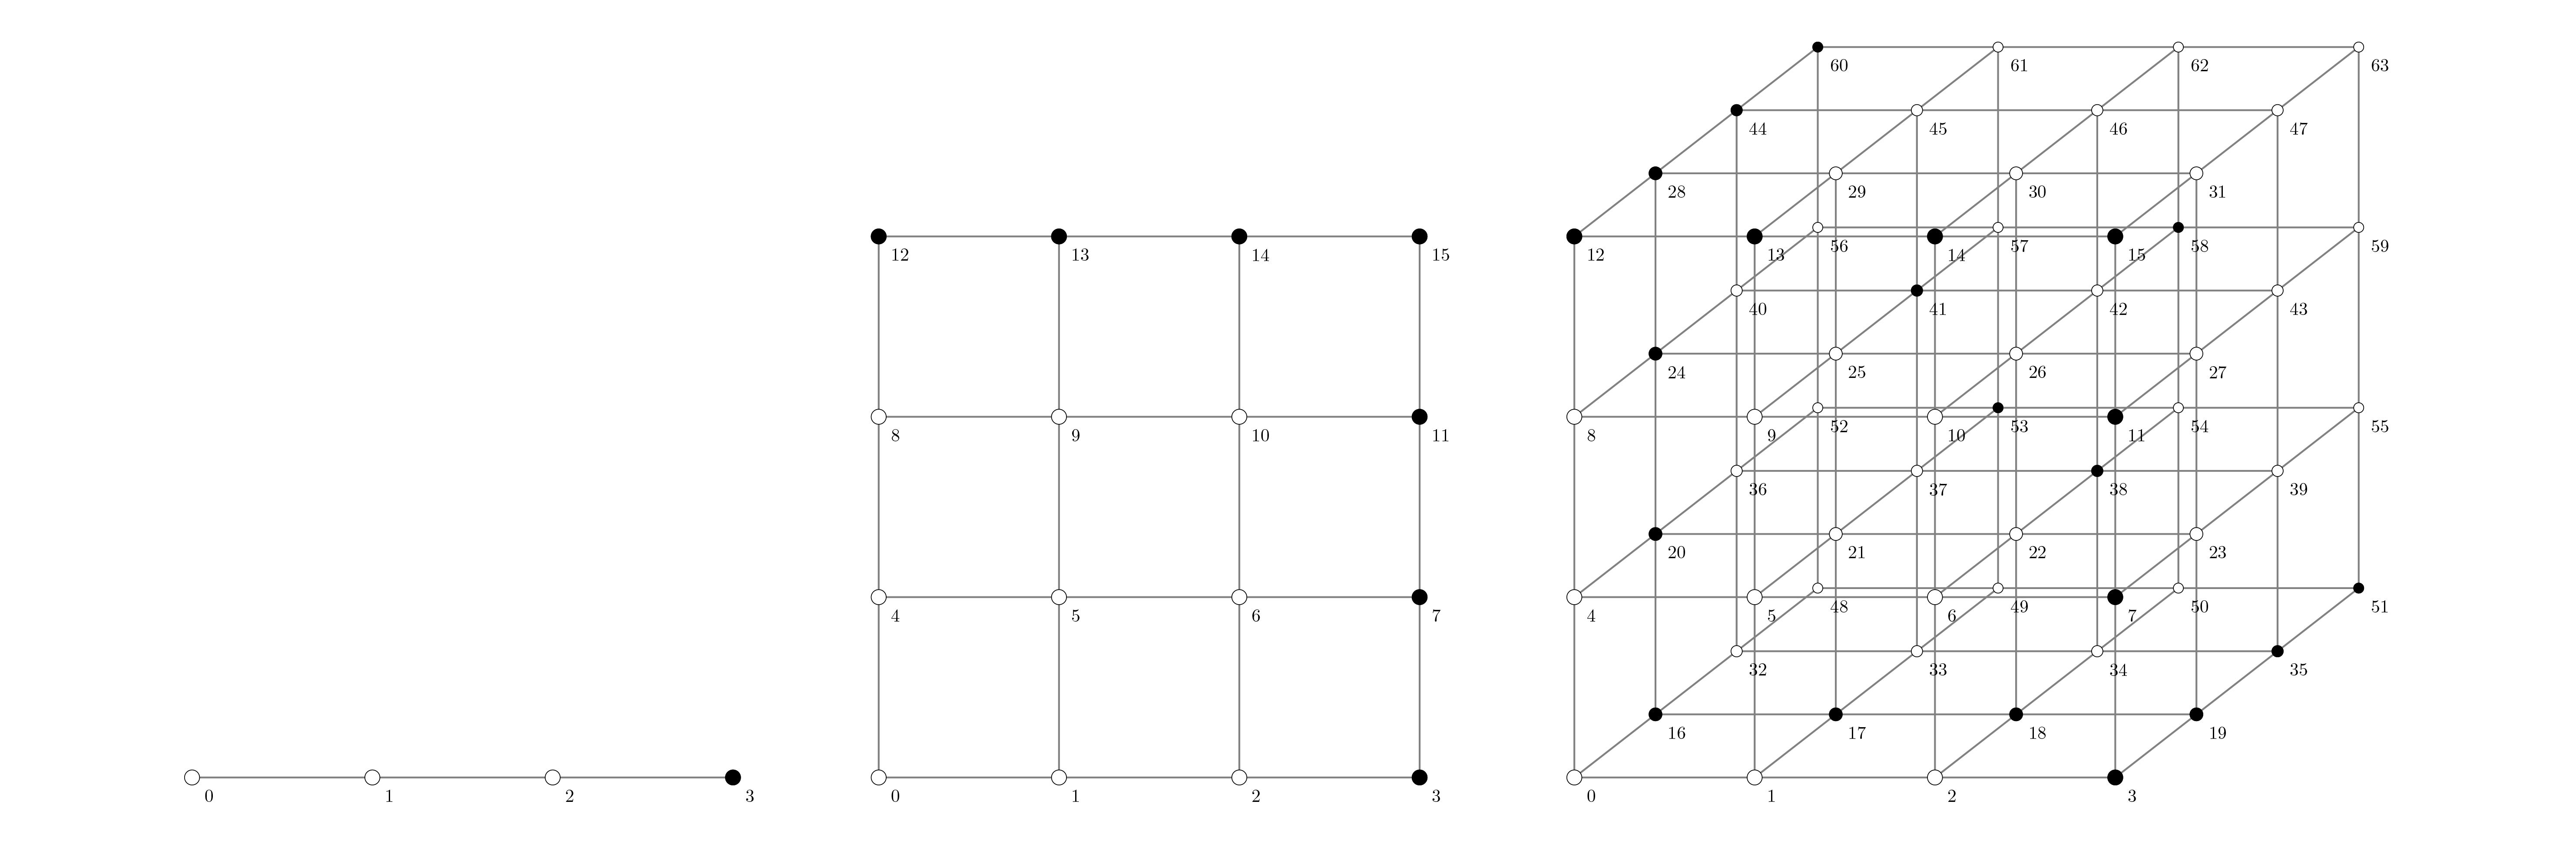
\includegraphics[width=0.12\textwidth]{cover}}

%----------------------------------------
% Configurations
%----------------------------------------

\graphicspath{{figures/}}

% \AtBeginSection
% {
% 	\begin{frame}<beamer>
% 		\vfill{}
% 		\centering
% 		\begin{beamercolorbox}[sep=8pt,center]{title}
% 			\Huge\insertsectionhead\par%
% 		\end{beamercolorbox}
% 		\vfill{}
% 	\end{frame}
% }

\AtBeginSection
{
	\begin{frame}[plain]
		\utbmtitle{\insertsectionhead}
	\end{frame}
}

\makeatletter
\let\@@magyar@captionfix\relax
\makeatother

%----------------------------------------
% Figures configuration
%----------------------------------------

\usetikzlibrary{shapes.geometric}
\usetikzlibrary{arrows.meta}
\usetikzlibrary{calc}
\usetikzlibrary{matrix}
\usetikzlibrary{fit}

\pgfmathsetmacro\pointsPerLine{4}

%---------------------------------
% Colors
\colorlet{points_boder_color}{black}%
\colorlet{points_color}{white}%
\colorlet{in_points_color}{black}%
\colorlet{lines_color}{gray}%

%---------------------------------
% Sizes
\pgfmathsetmacro\pointssep{100}%
\pgfmathsetmacro\pointssize{10}%
\pgfmathsetmacro\thepointssize{15}%
\pgfmathsetmacro\lineswidth{1}%

\newcommand{\inPoints}{}
\newcommand{\thePoints}{}

%----------------------------------------
% Document
%----------------------------------------
\begin{document}
	\begin{frame}[plain,noframenumbering]
		\titlepage
	\end{frame}
	% \begin{frame}{Table of contents}
	% 	\tableofcontents
	% \end{frame}
	%!TEX root = ./main.tex

\newsavebox\truehyperplane
\sbox{\truehyperplane}{%
	\pgfmathsetmacro\dimension{2}% in [0,3]
	\renewcommand{\inPoints}{0,1,2,3,4,8,12}%
	%---------------------------------
% Auto config
\pgfmathsetmacro\xdim{\dimension>0}%
\pgfmathsetmacro\ydim{\dimension>1}%
\pgfmathsetmacro\zdim{\dimension>2}%
\pgfmathsetmacro\pointsPerLineMinusOne{\pointsPerLine-1}%
\pgfmathsetmacro\xnbr{\pointsPerLineMinusOne*\xdim}%
\pgfmathsetmacro\ynbr{\pointsPerLineMinusOne*\ydim}%
\pgfmathsetmacro\znbr{\pointsPerLineMinusOne*\zdim}%

%---------------------------------
% Figure
\begin{tikzpicture}[x={(1pt,0pt)},y={(0pt,1pt)},z={(0.45pt,0.35pt)}]
	\tikzset{point/.style={
		draw,
		circle,
		minimum size=\pointsize,
		inner sep=0,
	}}

	% Coordinates
	\foreach \x in {0,...,\xnbr}
	{
		\foreach \y in {0,...,\ynbr}
		{
			\foreach \z in {0,...,\znbr}
			{
				\pgfmathsetmacro\num{int(\x+(\pointsPerLine*\y)+(\pointsPerLine*\pointsPerLine*\z))}
				\coordinate (point\num) at (\pointssep*\x,\pointssep*\y,\pointssep*\z) {};
				\coordinate (point_\x_\y_\z) at (\pointssep*\x,\pointssep*\y,\pointssep*\z) {};
			}
		}
	}

	% Lines
	\foreach \x in {0,...,\xnbr}
	{
		\foreach \y in {0,...,\ynbr}
		{
			\foreach \z in {0,...,\znbr}
			{
				\ifthenelse{\x=0}{}{
					\pgfmathsetmacro\lastx{int(\x-1)}
					\draw[line width=\lineswidth,lines_color] (point_\lastx_\y_\z) -- (point_\x_\y_\z);
				}
				\ifthenelse{\y=0}{}{
					\pgfmathsetmacro\lasty{int(\y-1)}
					\draw[line width=\lineswidth,lines_color] (point_\x_\lasty_\z) -- (point_\x_\y_\z);
				}
				\ifthenelse{\z=0}{}{
					\pgfmathsetmacro\lastz{int(\z-1)}
					\draw[line width=\lineswidth,lines_color] (point_\x_\y_\lastz) -- (point_\x_\y_\z);
				}
			}
		}
	}

	% Points and numbers
	\foreach \x in {0,...,\xnbr}
	{
		\foreach \y in {0,...,\ynbr}
		{
			\foreach \z in {0,...,\znbr}
			{
				% Config
				\pgfmathsetmacro\num{int(\x+(\pointsPerLine*\y)+(\pointsPerLine*\pointsPerLine*\z))}
				\pgfmathsetmacro\pointsize{\pointssize*5/(5+\z+1)}

				% Draw point
				\node[
					point,
					points_boder_color,
					fill=points_color
				] at (point_\x_\y_\z.center) {};

				% Fill point if is in
				\foreach \i in \inPoints
				{
					\ifthenelse{\num=\i}{
						\node[
							point,
							points_boder_color,
							fill=in_points_color
						] at (point\i.center) {};
					}{}
				}

				% Number
				\pgfmathsetmacro\num{int(\x+(\pointsPerLine*\y)+(\pointsPerLine*\pointsPerLine*\z))}
				\node[below right=3pt] at (point_\x_\y_\z.center) {\small\num};
			}
		}
	}
\end{tikzpicture}
%
}

\begin{frame}
	\frametitle{Definition}
	\begin{block}{Geometric hyperplane}
		An hyperplane $H$ is a proper subspace of $S_k(3)$ such that for each line of $S_k(3)$, $H$ either contain the full line or only one point of the line.
	\end{block}
	\centering%
	\resizebox{0.7\textwidth}{!}{
		\begin{tikzpicture}
			\node (falsehyperplane) at (0,0) {%!TEX root = ../main.tex

\pgfmathsetmacro\dimension{2}% in [0,3]
\renewcommand{\inPoints}{1,2,4,9,15}%

%---------------------------------
% Auto config
\pgfmathsetmacro\xdim{\dimension>0}%
\pgfmathsetmacro\ydim{\dimension>1}%
\pgfmathsetmacro\zdim{\dimension>2}%
\pgfmathsetmacro\pointsPerLineMinusOne{\pointsPerLine-1}%
\pgfmathsetmacro\xnbr{\pointsPerLineMinusOne*\xdim}%
\pgfmathsetmacro\ynbr{\pointsPerLineMinusOne*\ydim}%
\pgfmathsetmacro\znbr{\pointsPerLineMinusOne*\zdim}%

%---------------------------------
% Figure
\begin{tikzpicture}[x={(1pt,0pt)},y={(0pt,1pt)},z={(0.45pt,0.35pt)}]
	\tikzset{point/.style={
		draw,
		circle,
		minimum size=\pointsize,
		inner sep=0,
	}}

	% Coordinates
	\foreach \x in {0,...,\xnbr}
	{
		\foreach \y in {0,...,\ynbr}
		{
			\foreach \z in {0,...,\znbr}
			{
				\pgfmathsetmacro\num{int(\x+(\pointsPerLine*\y)+(\pointsPerLine*\pointsPerLine*\z))}
				\coordinate (point\num) at (\pointssep*\x,\pointssep*\y,\pointssep*\z) {};
				\coordinate (point_\x_\y_\z) at (\pointssep*\x,\pointssep*\y,\pointssep*\z) {};
			}
		}
	}

	\uncover<2->{

		% Lines
		\foreach \x in {0,...,\xnbr}
		{
			\foreach \y in {0,...,\ynbr}
			{
				\foreach \z in {0,...,\znbr}
				{
					\ifthenelse{\x=0}{}{
						\pgfmathsetmacro\lastx{int(\x-1)}
						\draw[line width=\lineswidth,lines_color] (point_\lastx_\y_\z) -- (point_\x_\y_\z);
					}
					\ifthenelse{\y=0}{}{
						\pgfmathsetmacro\lasty{int(\y-1)}
						\draw[line width=\lineswidth,lines_color] (point_\x_\lasty_\z) -- (point_\x_\y_\z);
					}
					\ifthenelse{\z=0}{}{
						\pgfmathsetmacro\lastz{int(\z-1)}
						\draw[line width=\lineswidth,lines_color] (point_\x_\y_\lastz) -- (point_\x_\y_\z);
					}
				}
			}
		}

		% Points and numbers
		\foreach \x in {0,...,\xnbr}
		{
			\foreach \y in {0,...,\ynbr}
			{
				\foreach \z in {0,...,\znbr}
				{
					% Config
					\pgfmathsetmacro\num{int(\x+(\pointsPerLine*\y)+(\pointsPerLine*\pointsPerLine*\z))}
					\pgfmathsetmacro\pointsize{\pointssize*5/(5+\z+1)}

					% Draw point
					\node[
						point,
						points_boder_color,
						fill=points_color
					] at (point_\x_\y_\z.center) {};

					% Fill point if is in
					\foreach \i in \inPoints
					{
						\ifthenelse{\num=\i}{
							\node[
								point,
								points_boder_color,
								fill=in_points_color
							] at (point\i.center) {};
						}{}
					}

					% Number
					\pgfmathsetmacro\num{int(\x+(\pointsPerLine*\y)+(\pointsPerLine*\pointsPerLine*\z))}
					\node[below right=3pt] at (point_\x_\y_\z.center) {\small\num};
				}
			}
		}

	}

	\uncover<3->{
		\node[fit=(point_1_0_0)(point_2_0_0), draw, ultra thick, red, ellipse, minimum height=20] {};
	}
	\uncover<4->{
		\draw[ultra thick, red] (point_0_0_0.center) -- (point_3_3_0.center);
		\draw[ultra thick, red] (point_3_0_0.center) -- (point_0_3_0.center);
	}
\end{tikzpicture}
};
			\uncover<2->{
				\node[anchor=south west, xshift=50] (truehyperplane) at (falsehyperplane.south east) {\usebox{\truehyperplane}};
			}
		\end{tikzpicture}
	}
\end{frame}

	%!TEX root = ./main.tex

%---------------------------------
% Geometry
\pgfmathsetmacro\dimension{2}% in [0,3]
\pgfmathsetmacro\pointsPerLine{4}% in [1,\infty[

\begin{frame}
	\frametitle{Dimension 2 hyperplanes}
	\renewcommand{\inPoints}{3,6,9,12}%
	\resizebox{0.09\textwidth}{!}{%---------------------------------
% Auto config
\pgfmathsetmacro\xdim{\dimension>0}%
\pgfmathsetmacro\ydim{\dimension>1}%
\pgfmathsetmacro\zdim{\dimension>2}%
\pgfmathsetmacro\pointsPerLineMinusOne{\pointsPerLine-1}%
\pgfmathsetmacro\xnbr{\pointsPerLineMinusOne*\xdim}%
\pgfmathsetmacro\ynbr{\pointsPerLineMinusOne*\ydim}%
\pgfmathsetmacro\znbr{\pointsPerLineMinusOne*\zdim}%

%---------------------------------
% Figure
\begin{tikzpicture}[x={(1pt,0pt)},y={(0pt,1pt)},z={(0.45pt,0.35pt)}]
	\tikzset{point/.style={
		draw,
		circle,
		minimum size=\pointsize,
		inner sep=0,
	}}

	% Coordinates
	\foreach \x in {0,...,\xnbr}
	{
		\foreach \y in {0,...,\ynbr}
		{
			\foreach \z in {0,...,\znbr}
			{
				\pgfmathsetmacro\num{int(\x+(\pointsPerLine*\y)+(\pointsPerLine*\pointsPerLine*\z))}
				\coordinate (point\num) at (\pointssep*\x,\pointssep*\y,\pointssep*\z) {};
				\coordinate (point_\x_\y_\z) at (\pointssep*\x,\pointssep*\y,\pointssep*\z) {};
			}
		}
	}

	% Lines
	\foreach \x in {0,...,\xnbr}
	{
		\foreach \y in {0,...,\ynbr}
		{
			\foreach \z in {0,...,\znbr}
			{
				\ifthenelse{\x=0}{}{
					\pgfmathsetmacro\lastx{int(\x-1)}
					\draw[line width=\lineswidth,lines_color] (point_\lastx_\y_\z) -- (point_\x_\y_\z);
				}
				\ifthenelse{\y=0}{}{
					\pgfmathsetmacro\lasty{int(\y-1)}
					\draw[line width=\lineswidth,lines_color] (point_\x_\lasty_\z) -- (point_\x_\y_\z);
				}
				\ifthenelse{\z=0}{}{
					\pgfmathsetmacro\lastz{int(\z-1)}
					\draw[line width=\lineswidth,lines_color] (point_\x_\y_\lastz) -- (point_\x_\y_\z);
				}
			}
		}
	}

	% Points and numbers
	\foreach \x in {0,...,\xnbr}
	{
		\foreach \y in {0,...,\ynbr}
		{
			\foreach \z in {0,...,\znbr}
			{
				% Config
				\pgfmathsetmacro\num{int(\x+(\pointsPerLine*\y)+(\pointsPerLine*\pointsPerLine*\z))}
				\pgfmathsetmacro\pointsize{\pointssize*5/(5+\z+1)}

				% Draw point
				\node[
					point,
					points_boder_color,
					fill=points_color
				] at (point_\x_\y_\z.center) {};

				% Fill point if is in
				\foreach \i in \inPoints
				{
					\ifthenelse{\num=\i}{
						\node[
							point,
							points_boder_color,
							fill=in_points_color
						] at (point\i.center) {};
					}{}
				}

				% Number
				\pgfmathsetmacro\num{int(\x+(\pointsPerLine*\y)+(\pointsPerLine*\pointsPerLine*\z))}
				\node[below right=3pt] at (point_\x_\y_\z.center) {\small\num};
			}
		}
	}
\end{tikzpicture}
}
	\renewcommand{\inPoints}{2,7,9,12}%
	\resizebox{0.09\textwidth}{!}{%---------------------------------
% Auto config
\pgfmathsetmacro\xdim{\dimension>0}%
\pgfmathsetmacro\ydim{\dimension>1}%
\pgfmathsetmacro\zdim{\dimension>2}%
\pgfmathsetmacro\pointsPerLineMinusOne{\pointsPerLine-1}%
\pgfmathsetmacro\xnbr{\pointsPerLineMinusOne*\xdim}%
\pgfmathsetmacro\ynbr{\pointsPerLineMinusOne*\ydim}%
\pgfmathsetmacro\znbr{\pointsPerLineMinusOne*\zdim}%

%---------------------------------
% Figure
\begin{tikzpicture}[x={(1pt,0pt)},y={(0pt,1pt)},z={(0.45pt,0.35pt)}]
	\tikzset{point/.style={
		draw,
		circle,
		minimum size=\pointsize,
		inner sep=0,
	}}

	% Coordinates
	\foreach \x in {0,...,\xnbr}
	{
		\foreach \y in {0,...,\ynbr}
		{
			\foreach \z in {0,...,\znbr}
			{
				\pgfmathsetmacro\num{int(\x+(\pointsPerLine*\y)+(\pointsPerLine*\pointsPerLine*\z))}
				\coordinate (point\num) at (\pointssep*\x,\pointssep*\y,\pointssep*\z) {};
				\coordinate (point_\x_\y_\z) at (\pointssep*\x,\pointssep*\y,\pointssep*\z) {};
			}
		}
	}

	% Lines
	\foreach \x in {0,...,\xnbr}
	{
		\foreach \y in {0,...,\ynbr}
		{
			\foreach \z in {0,...,\znbr}
			{
				\ifthenelse{\x=0}{}{
					\pgfmathsetmacro\lastx{int(\x-1)}
					\draw[line width=\lineswidth,lines_color] (point_\lastx_\y_\z) -- (point_\x_\y_\z);
				}
				\ifthenelse{\y=0}{}{
					\pgfmathsetmacro\lasty{int(\y-1)}
					\draw[line width=\lineswidth,lines_color] (point_\x_\lasty_\z) -- (point_\x_\y_\z);
				}
				\ifthenelse{\z=0}{}{
					\pgfmathsetmacro\lastz{int(\z-1)}
					\draw[line width=\lineswidth,lines_color] (point_\x_\y_\lastz) -- (point_\x_\y_\z);
				}
			}
		}
	}

	% Points and numbers
	\foreach \x in {0,...,\xnbr}
	{
		\foreach \y in {0,...,\ynbr}
		{
			\foreach \z in {0,...,\znbr}
			{
				% Config
				\pgfmathsetmacro\num{int(\x+(\pointsPerLine*\y)+(\pointsPerLine*\pointsPerLine*\z))}
				\pgfmathsetmacro\pointsize{\pointssize*5/(5+\z+1)}

				% Draw point
				\node[
					point,
					points_boder_color,
					fill=points_color
				] at (point_\x_\y_\z.center) {};

				% Fill point if is in
				\foreach \i in \inPoints
				{
					\ifthenelse{\num=\i}{
						\node[
							point,
							points_boder_color,
							fill=in_points_color
						] at (point\i.center) {};
					}{}
				}

				% Number
				\pgfmathsetmacro\num{int(\x+(\pointsPerLine*\y)+(\pointsPerLine*\pointsPerLine*\z))}
				\node[below right=3pt] at (point_\x_\y_\z.center) {\small\num};
			}
		}
	}
\end{tikzpicture}
}
	\renewcommand{\inPoints}{3,5,10,12}%
	\resizebox{0.09\textwidth}{!}{%---------------------------------
% Auto config
\pgfmathsetmacro\xdim{\dimension>0}%
\pgfmathsetmacro\ydim{\dimension>1}%
\pgfmathsetmacro\zdim{\dimension>2}%
\pgfmathsetmacro\pointsPerLineMinusOne{\pointsPerLine-1}%
\pgfmathsetmacro\xnbr{\pointsPerLineMinusOne*\xdim}%
\pgfmathsetmacro\ynbr{\pointsPerLineMinusOne*\ydim}%
\pgfmathsetmacro\znbr{\pointsPerLineMinusOne*\zdim}%

%---------------------------------
% Figure
\begin{tikzpicture}[x={(1pt,0pt)},y={(0pt,1pt)},z={(0.45pt,0.35pt)}]
	\tikzset{point/.style={
		draw,
		circle,
		minimum size=\pointsize,
		inner sep=0,
	}}

	% Coordinates
	\foreach \x in {0,...,\xnbr}
	{
		\foreach \y in {0,...,\ynbr}
		{
			\foreach \z in {0,...,\znbr}
			{
				\pgfmathsetmacro\num{int(\x+(\pointsPerLine*\y)+(\pointsPerLine*\pointsPerLine*\z))}
				\coordinate (point\num) at (\pointssep*\x,\pointssep*\y,\pointssep*\z) {};
				\coordinate (point_\x_\y_\z) at (\pointssep*\x,\pointssep*\y,\pointssep*\z) {};
			}
		}
	}

	% Lines
	\foreach \x in {0,...,\xnbr}
	{
		\foreach \y in {0,...,\ynbr}
		{
			\foreach \z in {0,...,\znbr}
			{
				\ifthenelse{\x=0}{}{
					\pgfmathsetmacro\lastx{int(\x-1)}
					\draw[line width=\lineswidth,lines_color] (point_\lastx_\y_\z) -- (point_\x_\y_\z);
				}
				\ifthenelse{\y=0}{}{
					\pgfmathsetmacro\lasty{int(\y-1)}
					\draw[line width=\lineswidth,lines_color] (point_\x_\lasty_\z) -- (point_\x_\y_\z);
				}
				\ifthenelse{\z=0}{}{
					\pgfmathsetmacro\lastz{int(\z-1)}
					\draw[line width=\lineswidth,lines_color] (point_\x_\y_\lastz) -- (point_\x_\y_\z);
				}
			}
		}
	}

	% Points and numbers
	\foreach \x in {0,...,\xnbr}
	{
		\foreach \y in {0,...,\ynbr}
		{
			\foreach \z in {0,...,\znbr}
			{
				% Config
				\pgfmathsetmacro\num{int(\x+(\pointsPerLine*\y)+(\pointsPerLine*\pointsPerLine*\z))}
				\pgfmathsetmacro\pointsize{\pointssize*5/(5+\z+1)}

				% Draw point
				\node[
					point,
					points_boder_color,
					fill=points_color
				] at (point_\x_\y_\z.center) {};

				% Fill point if is in
				\foreach \i in \inPoints
				{
					\ifthenelse{\num=\i}{
						\node[
							point,
							points_boder_color,
							fill=in_points_color
						] at (point\i.center) {};
					}{}
				}

				% Number
				\pgfmathsetmacro\num{int(\x+(\pointsPerLine*\y)+(\pointsPerLine*\pointsPerLine*\z))}
				\node[below right=3pt] at (point_\x_\y_\z.center) {\small\num};
			}
		}
	}
\end{tikzpicture}
}
	\renewcommand{\inPoints}{1,7,10,12}%
	\resizebox{0.09\textwidth}{!}{%---------------------------------
% Auto config
\pgfmathsetmacro\xdim{\dimension>0}%
\pgfmathsetmacro\ydim{\dimension>1}%
\pgfmathsetmacro\zdim{\dimension>2}%
\pgfmathsetmacro\pointsPerLineMinusOne{\pointsPerLine-1}%
\pgfmathsetmacro\xnbr{\pointsPerLineMinusOne*\xdim}%
\pgfmathsetmacro\ynbr{\pointsPerLineMinusOne*\ydim}%
\pgfmathsetmacro\znbr{\pointsPerLineMinusOne*\zdim}%

%---------------------------------
% Figure
\begin{tikzpicture}[x={(1pt,0pt)},y={(0pt,1pt)},z={(0.45pt,0.35pt)}]
	\tikzset{point/.style={
		draw,
		circle,
		minimum size=\pointsize,
		inner sep=0,
	}}

	% Coordinates
	\foreach \x in {0,...,\xnbr}
	{
		\foreach \y in {0,...,\ynbr}
		{
			\foreach \z in {0,...,\znbr}
			{
				\pgfmathsetmacro\num{int(\x+(\pointsPerLine*\y)+(\pointsPerLine*\pointsPerLine*\z))}
				\coordinate (point\num) at (\pointssep*\x,\pointssep*\y,\pointssep*\z) {};
				\coordinate (point_\x_\y_\z) at (\pointssep*\x,\pointssep*\y,\pointssep*\z) {};
			}
		}
	}

	% Lines
	\foreach \x in {0,...,\xnbr}
	{
		\foreach \y in {0,...,\ynbr}
		{
			\foreach \z in {0,...,\znbr}
			{
				\ifthenelse{\x=0}{}{
					\pgfmathsetmacro\lastx{int(\x-1)}
					\draw[line width=\lineswidth,lines_color] (point_\lastx_\y_\z) -- (point_\x_\y_\z);
				}
				\ifthenelse{\y=0}{}{
					\pgfmathsetmacro\lasty{int(\y-1)}
					\draw[line width=\lineswidth,lines_color] (point_\x_\lasty_\z) -- (point_\x_\y_\z);
				}
				\ifthenelse{\z=0}{}{
					\pgfmathsetmacro\lastz{int(\z-1)}
					\draw[line width=\lineswidth,lines_color] (point_\x_\y_\lastz) -- (point_\x_\y_\z);
				}
			}
		}
	}

	% Points and numbers
	\foreach \x in {0,...,\xnbr}
	{
		\foreach \y in {0,...,\ynbr}
		{
			\foreach \z in {0,...,\znbr}
			{
				% Config
				\pgfmathsetmacro\num{int(\x+(\pointsPerLine*\y)+(\pointsPerLine*\pointsPerLine*\z))}
				\pgfmathsetmacro\pointsize{\pointssize*5/(5+\z+1)}

				% Draw point
				\node[
					point,
					points_boder_color,
					fill=points_color
				] at (point_\x_\y_\z.center) {};

				% Fill point if is in
				\foreach \i in \inPoints
				{
					\ifthenelse{\num=\i}{
						\node[
							point,
							points_boder_color,
							fill=in_points_color
						] at (point\i.center) {};
					}{}
				}

				% Number
				\pgfmathsetmacro\num{int(\x+(\pointsPerLine*\y)+(\pointsPerLine*\pointsPerLine*\z))}
				\node[below right=3pt] at (point_\x_\y_\z.center) {\small\num};
			}
		}
	}
\end{tikzpicture}
}
	\renewcommand{\inPoints}{2,5,11,12}%
	\resizebox{0.09\textwidth}{!}{%---------------------------------
% Auto config
\pgfmathsetmacro\xdim{\dimension>0}%
\pgfmathsetmacro\ydim{\dimension>1}%
\pgfmathsetmacro\zdim{\dimension>2}%
\pgfmathsetmacro\pointsPerLineMinusOne{\pointsPerLine-1}%
\pgfmathsetmacro\xnbr{\pointsPerLineMinusOne*\xdim}%
\pgfmathsetmacro\ynbr{\pointsPerLineMinusOne*\ydim}%
\pgfmathsetmacro\znbr{\pointsPerLineMinusOne*\zdim}%

%---------------------------------
% Figure
\begin{tikzpicture}[x={(1pt,0pt)},y={(0pt,1pt)},z={(0.45pt,0.35pt)}]
	\tikzset{point/.style={
		draw,
		circle,
		minimum size=\pointsize,
		inner sep=0,
	}}

	% Coordinates
	\foreach \x in {0,...,\xnbr}
	{
		\foreach \y in {0,...,\ynbr}
		{
			\foreach \z in {0,...,\znbr}
			{
				\pgfmathsetmacro\num{int(\x+(\pointsPerLine*\y)+(\pointsPerLine*\pointsPerLine*\z))}
				\coordinate (point\num) at (\pointssep*\x,\pointssep*\y,\pointssep*\z) {};
				\coordinate (point_\x_\y_\z) at (\pointssep*\x,\pointssep*\y,\pointssep*\z) {};
			}
		}
	}

	% Lines
	\foreach \x in {0,...,\xnbr}
	{
		\foreach \y in {0,...,\ynbr}
		{
			\foreach \z in {0,...,\znbr}
			{
				\ifthenelse{\x=0}{}{
					\pgfmathsetmacro\lastx{int(\x-1)}
					\draw[line width=\lineswidth,lines_color] (point_\lastx_\y_\z) -- (point_\x_\y_\z);
				}
				\ifthenelse{\y=0}{}{
					\pgfmathsetmacro\lasty{int(\y-1)}
					\draw[line width=\lineswidth,lines_color] (point_\x_\lasty_\z) -- (point_\x_\y_\z);
				}
				\ifthenelse{\z=0}{}{
					\pgfmathsetmacro\lastz{int(\z-1)}
					\draw[line width=\lineswidth,lines_color] (point_\x_\y_\lastz) -- (point_\x_\y_\z);
				}
			}
		}
	}

	% Points and numbers
	\foreach \x in {0,...,\xnbr}
	{
		\foreach \y in {0,...,\ynbr}
		{
			\foreach \z in {0,...,\znbr}
			{
				% Config
				\pgfmathsetmacro\num{int(\x+(\pointsPerLine*\y)+(\pointsPerLine*\pointsPerLine*\z))}
				\pgfmathsetmacro\pointsize{\pointssize*5/(5+\z+1)}

				% Draw point
				\node[
					point,
					points_boder_color,
					fill=points_color
				] at (point_\x_\y_\z.center) {};

				% Fill point if is in
				\foreach \i in \inPoints
				{
					\ifthenelse{\num=\i}{
						\node[
							point,
							points_boder_color,
							fill=in_points_color
						] at (point\i.center) {};
					}{}
				}

				% Number
				\pgfmathsetmacro\num{int(\x+(\pointsPerLine*\y)+(\pointsPerLine*\pointsPerLine*\z))}
				\node[below right=3pt] at (point_\x_\y_\z.center) {\small\num};
			}
		}
	}
\end{tikzpicture}
}
	\renewcommand{\inPoints}{1,6,11,12}%
	\resizebox{0.09\textwidth}{!}{%---------------------------------
% Auto config
\pgfmathsetmacro\xdim{\dimension>0}%
\pgfmathsetmacro\ydim{\dimension>1}%
\pgfmathsetmacro\zdim{\dimension>2}%
\pgfmathsetmacro\pointsPerLineMinusOne{\pointsPerLine-1}%
\pgfmathsetmacro\xnbr{\pointsPerLineMinusOne*\xdim}%
\pgfmathsetmacro\ynbr{\pointsPerLineMinusOne*\ydim}%
\pgfmathsetmacro\znbr{\pointsPerLineMinusOne*\zdim}%

%---------------------------------
% Figure
\begin{tikzpicture}[x={(1pt,0pt)},y={(0pt,1pt)},z={(0.45pt,0.35pt)}]
	\tikzset{point/.style={
		draw,
		circle,
		minimum size=\pointsize,
		inner sep=0,
	}}

	% Coordinates
	\foreach \x in {0,...,\xnbr}
	{
		\foreach \y in {0,...,\ynbr}
		{
			\foreach \z in {0,...,\znbr}
			{
				\pgfmathsetmacro\num{int(\x+(\pointsPerLine*\y)+(\pointsPerLine*\pointsPerLine*\z))}
				\coordinate (point\num) at (\pointssep*\x,\pointssep*\y,\pointssep*\z) {};
				\coordinate (point_\x_\y_\z) at (\pointssep*\x,\pointssep*\y,\pointssep*\z) {};
			}
		}
	}

	% Lines
	\foreach \x in {0,...,\xnbr}
	{
		\foreach \y in {0,...,\ynbr}
		{
			\foreach \z in {0,...,\znbr}
			{
				\ifthenelse{\x=0}{}{
					\pgfmathsetmacro\lastx{int(\x-1)}
					\draw[line width=\lineswidth,lines_color] (point_\lastx_\y_\z) -- (point_\x_\y_\z);
				}
				\ifthenelse{\y=0}{}{
					\pgfmathsetmacro\lasty{int(\y-1)}
					\draw[line width=\lineswidth,lines_color] (point_\x_\lasty_\z) -- (point_\x_\y_\z);
				}
				\ifthenelse{\z=0}{}{
					\pgfmathsetmacro\lastz{int(\z-1)}
					\draw[line width=\lineswidth,lines_color] (point_\x_\y_\lastz) -- (point_\x_\y_\z);
				}
			}
		}
	}

	% Points and numbers
	\foreach \x in {0,...,\xnbr}
	{
		\foreach \y in {0,...,\ynbr}
		{
			\foreach \z in {0,...,\znbr}
			{
				% Config
				\pgfmathsetmacro\num{int(\x+(\pointsPerLine*\y)+(\pointsPerLine*\pointsPerLine*\z))}
				\pgfmathsetmacro\pointsize{\pointssize*5/(5+\z+1)}

				% Draw point
				\node[
					point,
					points_boder_color,
					fill=points_color
				] at (point_\x_\y_\z.center) {};

				% Fill point if is in
				\foreach \i in \inPoints
				{
					\ifthenelse{\num=\i}{
						\node[
							point,
							points_boder_color,
							fill=in_points_color
						] at (point\i.center) {};
					}{}
				}

				% Number
				\pgfmathsetmacro\num{int(\x+(\pointsPerLine*\y)+(\pointsPerLine*\pointsPerLine*\z))}
				\node[below right=3pt] at (point_\x_\y_\z.center) {\small\num};
			}
		}
	}
\end{tikzpicture}
}
	\renewcommand{\inPoints}{3,6,8,13}%
	\resizebox{0.09\textwidth}{!}{%---------------------------------
% Auto config
\pgfmathsetmacro\xdim{\dimension>0}%
\pgfmathsetmacro\ydim{\dimension>1}%
\pgfmathsetmacro\zdim{\dimension>2}%
\pgfmathsetmacro\pointsPerLineMinusOne{\pointsPerLine-1}%
\pgfmathsetmacro\xnbr{\pointsPerLineMinusOne*\xdim}%
\pgfmathsetmacro\ynbr{\pointsPerLineMinusOne*\ydim}%
\pgfmathsetmacro\znbr{\pointsPerLineMinusOne*\zdim}%

%---------------------------------
% Figure
\begin{tikzpicture}[x={(1pt,0pt)},y={(0pt,1pt)},z={(0.45pt,0.35pt)}]
	\tikzset{point/.style={
		draw,
		circle,
		minimum size=\pointsize,
		inner sep=0,
	}}

	% Coordinates
	\foreach \x in {0,...,\xnbr}
	{
		\foreach \y in {0,...,\ynbr}
		{
			\foreach \z in {0,...,\znbr}
			{
				\pgfmathsetmacro\num{int(\x+(\pointsPerLine*\y)+(\pointsPerLine*\pointsPerLine*\z))}
				\coordinate (point\num) at (\pointssep*\x,\pointssep*\y,\pointssep*\z) {};
				\coordinate (point_\x_\y_\z) at (\pointssep*\x,\pointssep*\y,\pointssep*\z) {};
			}
		}
	}

	% Lines
	\foreach \x in {0,...,\xnbr}
	{
		\foreach \y in {0,...,\ynbr}
		{
			\foreach \z in {0,...,\znbr}
			{
				\ifthenelse{\x=0}{}{
					\pgfmathsetmacro\lastx{int(\x-1)}
					\draw[line width=\lineswidth,lines_color] (point_\lastx_\y_\z) -- (point_\x_\y_\z);
				}
				\ifthenelse{\y=0}{}{
					\pgfmathsetmacro\lasty{int(\y-1)}
					\draw[line width=\lineswidth,lines_color] (point_\x_\lasty_\z) -- (point_\x_\y_\z);
				}
				\ifthenelse{\z=0}{}{
					\pgfmathsetmacro\lastz{int(\z-1)}
					\draw[line width=\lineswidth,lines_color] (point_\x_\y_\lastz) -- (point_\x_\y_\z);
				}
			}
		}
	}

	% Points and numbers
	\foreach \x in {0,...,\xnbr}
	{
		\foreach \y in {0,...,\ynbr}
		{
			\foreach \z in {0,...,\znbr}
			{
				% Config
				\pgfmathsetmacro\num{int(\x+(\pointsPerLine*\y)+(\pointsPerLine*\pointsPerLine*\z))}
				\pgfmathsetmacro\pointsize{\pointssize*5/(5+\z+1)}

				% Draw point
				\node[
					point,
					points_boder_color,
					fill=points_color
				] at (point_\x_\y_\z.center) {};

				% Fill point if is in
				\foreach \i in \inPoints
				{
					\ifthenelse{\num=\i}{
						\node[
							point,
							points_boder_color,
							fill=in_points_color
						] at (point\i.center) {};
					}{}
				}

				% Number
				\pgfmathsetmacro\num{int(\x+(\pointsPerLine*\y)+(\pointsPerLine*\pointsPerLine*\z))}
				\node[below right=3pt] at (point_\x_\y_\z.center) {\small\num};
			}
		}
	}
\end{tikzpicture}
}
	\renewcommand{\inPoints}{2,7,8,13}%
	\resizebox{0.09\textwidth}{!}{%---------------------------------
% Auto config
\pgfmathsetmacro\xdim{\dimension>0}%
\pgfmathsetmacro\ydim{\dimension>1}%
\pgfmathsetmacro\zdim{\dimension>2}%
\pgfmathsetmacro\pointsPerLineMinusOne{\pointsPerLine-1}%
\pgfmathsetmacro\xnbr{\pointsPerLineMinusOne*\xdim}%
\pgfmathsetmacro\ynbr{\pointsPerLineMinusOne*\ydim}%
\pgfmathsetmacro\znbr{\pointsPerLineMinusOne*\zdim}%

%---------------------------------
% Figure
\begin{tikzpicture}[x={(1pt,0pt)},y={(0pt,1pt)},z={(0.45pt,0.35pt)}]
	\tikzset{point/.style={
		draw,
		circle,
		minimum size=\pointsize,
		inner sep=0,
	}}

	% Coordinates
	\foreach \x in {0,...,\xnbr}
	{
		\foreach \y in {0,...,\ynbr}
		{
			\foreach \z in {0,...,\znbr}
			{
				\pgfmathsetmacro\num{int(\x+(\pointsPerLine*\y)+(\pointsPerLine*\pointsPerLine*\z))}
				\coordinate (point\num) at (\pointssep*\x,\pointssep*\y,\pointssep*\z) {};
				\coordinate (point_\x_\y_\z) at (\pointssep*\x,\pointssep*\y,\pointssep*\z) {};
			}
		}
	}

	% Lines
	\foreach \x in {0,...,\xnbr}
	{
		\foreach \y in {0,...,\ynbr}
		{
			\foreach \z in {0,...,\znbr}
			{
				\ifthenelse{\x=0}{}{
					\pgfmathsetmacro\lastx{int(\x-1)}
					\draw[line width=\lineswidth,lines_color] (point_\lastx_\y_\z) -- (point_\x_\y_\z);
				}
				\ifthenelse{\y=0}{}{
					\pgfmathsetmacro\lasty{int(\y-1)}
					\draw[line width=\lineswidth,lines_color] (point_\x_\lasty_\z) -- (point_\x_\y_\z);
				}
				\ifthenelse{\z=0}{}{
					\pgfmathsetmacro\lastz{int(\z-1)}
					\draw[line width=\lineswidth,lines_color] (point_\x_\y_\lastz) -- (point_\x_\y_\z);
				}
			}
		}
	}

	% Points and numbers
	\foreach \x in {0,...,\xnbr}
	{
		\foreach \y in {0,...,\ynbr}
		{
			\foreach \z in {0,...,\znbr}
			{
				% Config
				\pgfmathsetmacro\num{int(\x+(\pointsPerLine*\y)+(\pointsPerLine*\pointsPerLine*\z))}
				\pgfmathsetmacro\pointsize{\pointssize*5/(5+\z+1)}

				% Draw point
				\node[
					point,
					points_boder_color,
					fill=points_color
				] at (point_\x_\y_\z.center) {};

				% Fill point if is in
				\foreach \i in \inPoints
				{
					\ifthenelse{\num=\i}{
						\node[
							point,
							points_boder_color,
							fill=in_points_color
						] at (point\i.center) {};
					}{}
				}

				% Number
				\pgfmathsetmacro\num{int(\x+(\pointsPerLine*\y)+(\pointsPerLine*\pointsPerLine*\z))}
				\node[below right=3pt] at (point_\x_\y_\z.center) {\small\num};
			}
		}
	}
\end{tikzpicture}
}
	\renewcommand{\inPoints}{3,4,10,13}%
	\resizebox{0.09\textwidth}{!}{%---------------------------------
% Auto config
\pgfmathsetmacro\xdim{\dimension>0}%
\pgfmathsetmacro\ydim{\dimension>1}%
\pgfmathsetmacro\zdim{\dimension>2}%
\pgfmathsetmacro\pointsPerLineMinusOne{\pointsPerLine-1}%
\pgfmathsetmacro\xnbr{\pointsPerLineMinusOne*\xdim}%
\pgfmathsetmacro\ynbr{\pointsPerLineMinusOne*\ydim}%
\pgfmathsetmacro\znbr{\pointsPerLineMinusOne*\zdim}%

%---------------------------------
% Figure
\begin{tikzpicture}[x={(1pt,0pt)},y={(0pt,1pt)},z={(0.45pt,0.35pt)}]
	\tikzset{point/.style={
		draw,
		circle,
		minimum size=\pointsize,
		inner sep=0,
	}}

	% Coordinates
	\foreach \x in {0,...,\xnbr}
	{
		\foreach \y in {0,...,\ynbr}
		{
			\foreach \z in {0,...,\znbr}
			{
				\pgfmathsetmacro\num{int(\x+(\pointsPerLine*\y)+(\pointsPerLine*\pointsPerLine*\z))}
				\coordinate (point\num) at (\pointssep*\x,\pointssep*\y,\pointssep*\z) {};
				\coordinate (point_\x_\y_\z) at (\pointssep*\x,\pointssep*\y,\pointssep*\z) {};
			}
		}
	}

	% Lines
	\foreach \x in {0,...,\xnbr}
	{
		\foreach \y in {0,...,\ynbr}
		{
			\foreach \z in {0,...,\znbr}
			{
				\ifthenelse{\x=0}{}{
					\pgfmathsetmacro\lastx{int(\x-1)}
					\draw[line width=\lineswidth,lines_color] (point_\lastx_\y_\z) -- (point_\x_\y_\z);
				}
				\ifthenelse{\y=0}{}{
					\pgfmathsetmacro\lasty{int(\y-1)}
					\draw[line width=\lineswidth,lines_color] (point_\x_\lasty_\z) -- (point_\x_\y_\z);
				}
				\ifthenelse{\z=0}{}{
					\pgfmathsetmacro\lastz{int(\z-1)}
					\draw[line width=\lineswidth,lines_color] (point_\x_\y_\lastz) -- (point_\x_\y_\z);
				}
			}
		}
	}

	% Points and numbers
	\foreach \x in {0,...,\xnbr}
	{
		\foreach \y in {0,...,\ynbr}
		{
			\foreach \z in {0,...,\znbr}
			{
				% Config
				\pgfmathsetmacro\num{int(\x+(\pointsPerLine*\y)+(\pointsPerLine*\pointsPerLine*\z))}
				\pgfmathsetmacro\pointsize{\pointssize*5/(5+\z+1)}

				% Draw point
				\node[
					point,
					points_boder_color,
					fill=points_color
				] at (point_\x_\y_\z.center) {};

				% Fill point if is in
				\foreach \i in \inPoints
				{
					\ifthenelse{\num=\i}{
						\node[
							point,
							points_boder_color,
							fill=in_points_color
						] at (point\i.center) {};
					}{}
				}

				% Number
				\pgfmathsetmacro\num{int(\x+(\pointsPerLine*\y)+(\pointsPerLine*\pointsPerLine*\z))}
				\node[below right=3pt] at (point_\x_\y_\z.center) {\small\num};
			}
		}
	}
\end{tikzpicture}
}
	\renewcommand{\inPoints}{0,7,10,13}%
	\resizebox{0.09\textwidth}{!}{%---------------------------------
% Auto config
\pgfmathsetmacro\xdim{\dimension>0}%
\pgfmathsetmacro\ydim{\dimension>1}%
\pgfmathsetmacro\zdim{\dimension>2}%
\pgfmathsetmacro\pointsPerLineMinusOne{\pointsPerLine-1}%
\pgfmathsetmacro\xnbr{\pointsPerLineMinusOne*\xdim}%
\pgfmathsetmacro\ynbr{\pointsPerLineMinusOne*\ydim}%
\pgfmathsetmacro\znbr{\pointsPerLineMinusOne*\zdim}%

%---------------------------------
% Figure
\begin{tikzpicture}[x={(1pt,0pt)},y={(0pt,1pt)},z={(0.45pt,0.35pt)}]
	\tikzset{point/.style={
		draw,
		circle,
		minimum size=\pointsize,
		inner sep=0,
	}}

	% Coordinates
	\foreach \x in {0,...,\xnbr}
	{
		\foreach \y in {0,...,\ynbr}
		{
			\foreach \z in {0,...,\znbr}
			{
				\pgfmathsetmacro\num{int(\x+(\pointsPerLine*\y)+(\pointsPerLine*\pointsPerLine*\z))}
				\coordinate (point\num) at (\pointssep*\x,\pointssep*\y,\pointssep*\z) {};
				\coordinate (point_\x_\y_\z) at (\pointssep*\x,\pointssep*\y,\pointssep*\z) {};
			}
		}
	}

	% Lines
	\foreach \x in {0,...,\xnbr}
	{
		\foreach \y in {0,...,\ynbr}
		{
			\foreach \z in {0,...,\znbr}
			{
				\ifthenelse{\x=0}{}{
					\pgfmathsetmacro\lastx{int(\x-1)}
					\draw[line width=\lineswidth,lines_color] (point_\lastx_\y_\z) -- (point_\x_\y_\z);
				}
				\ifthenelse{\y=0}{}{
					\pgfmathsetmacro\lasty{int(\y-1)}
					\draw[line width=\lineswidth,lines_color] (point_\x_\lasty_\z) -- (point_\x_\y_\z);
				}
				\ifthenelse{\z=0}{}{
					\pgfmathsetmacro\lastz{int(\z-1)}
					\draw[line width=\lineswidth,lines_color] (point_\x_\y_\lastz) -- (point_\x_\y_\z);
				}
			}
		}
	}

	% Points and numbers
	\foreach \x in {0,...,\xnbr}
	{
		\foreach \y in {0,...,\ynbr}
		{
			\foreach \z in {0,...,\znbr}
			{
				% Config
				\pgfmathsetmacro\num{int(\x+(\pointsPerLine*\y)+(\pointsPerLine*\pointsPerLine*\z))}
				\pgfmathsetmacro\pointsize{\pointssize*5/(5+\z+1)}

				% Draw point
				\node[
					point,
					points_boder_color,
					fill=points_color
				] at (point_\x_\y_\z.center) {};

				% Fill point if is in
				\foreach \i in \inPoints
				{
					\ifthenelse{\num=\i}{
						\node[
							point,
							points_boder_color,
							fill=in_points_color
						] at (point\i.center) {};
					}{}
				}

				% Number
				\pgfmathsetmacro\num{int(\x+(\pointsPerLine*\y)+(\pointsPerLine*\pointsPerLine*\z))}
				\node[below right=3pt] at (point_\x_\y_\z.center) {\small\num};
			}
		}
	}
\end{tikzpicture}
}
	\renewcommand{\inPoints}{2,4,11,13}%
	\resizebox{0.09\textwidth}{!}{%---------------------------------
% Auto config
\pgfmathsetmacro\xdim{\dimension>0}%
\pgfmathsetmacro\ydim{\dimension>1}%
\pgfmathsetmacro\zdim{\dimension>2}%
\pgfmathsetmacro\pointsPerLineMinusOne{\pointsPerLine-1}%
\pgfmathsetmacro\xnbr{\pointsPerLineMinusOne*\xdim}%
\pgfmathsetmacro\ynbr{\pointsPerLineMinusOne*\ydim}%
\pgfmathsetmacro\znbr{\pointsPerLineMinusOne*\zdim}%

%---------------------------------
% Figure
\begin{tikzpicture}[x={(1pt,0pt)},y={(0pt,1pt)},z={(0.45pt,0.35pt)}]
	\tikzset{point/.style={
		draw,
		circle,
		minimum size=\pointsize,
		inner sep=0,
	}}

	% Coordinates
	\foreach \x in {0,...,\xnbr}
	{
		\foreach \y in {0,...,\ynbr}
		{
			\foreach \z in {0,...,\znbr}
			{
				\pgfmathsetmacro\num{int(\x+(\pointsPerLine*\y)+(\pointsPerLine*\pointsPerLine*\z))}
				\coordinate (point\num) at (\pointssep*\x,\pointssep*\y,\pointssep*\z) {};
				\coordinate (point_\x_\y_\z) at (\pointssep*\x,\pointssep*\y,\pointssep*\z) {};
			}
		}
	}

	% Lines
	\foreach \x in {0,...,\xnbr}
	{
		\foreach \y in {0,...,\ynbr}
		{
			\foreach \z in {0,...,\znbr}
			{
				\ifthenelse{\x=0}{}{
					\pgfmathsetmacro\lastx{int(\x-1)}
					\draw[line width=\lineswidth,lines_color] (point_\lastx_\y_\z) -- (point_\x_\y_\z);
				}
				\ifthenelse{\y=0}{}{
					\pgfmathsetmacro\lasty{int(\y-1)}
					\draw[line width=\lineswidth,lines_color] (point_\x_\lasty_\z) -- (point_\x_\y_\z);
				}
				\ifthenelse{\z=0}{}{
					\pgfmathsetmacro\lastz{int(\z-1)}
					\draw[line width=\lineswidth,lines_color] (point_\x_\y_\lastz) -- (point_\x_\y_\z);
				}
			}
		}
	}

	% Points and numbers
	\foreach \x in {0,...,\xnbr}
	{
		\foreach \y in {0,...,\ynbr}
		{
			\foreach \z in {0,...,\znbr}
			{
				% Config
				\pgfmathsetmacro\num{int(\x+(\pointsPerLine*\y)+(\pointsPerLine*\pointsPerLine*\z))}
				\pgfmathsetmacro\pointsize{\pointssize*5/(5+\z+1)}

				% Draw point
				\node[
					point,
					points_boder_color,
					fill=points_color
				] at (point_\x_\y_\z.center) {};

				% Fill point if is in
				\foreach \i in \inPoints
				{
					\ifthenelse{\num=\i}{
						\node[
							point,
							points_boder_color,
							fill=in_points_color
						] at (point\i.center) {};
					}{}
				}

				% Number
				\pgfmathsetmacro\num{int(\x+(\pointsPerLine*\y)+(\pointsPerLine*\pointsPerLine*\z))}
				\node[below right=3pt] at (point_\x_\y_\z.center) {\small\num};
			}
		}
	}
\end{tikzpicture}
}
	\renewcommand{\inPoints}{0,6,11,13}%
	\resizebox{0.09\textwidth}{!}{%---------------------------------
% Auto config
\pgfmathsetmacro\xdim{\dimension>0}%
\pgfmathsetmacro\ydim{\dimension>1}%
\pgfmathsetmacro\zdim{\dimension>2}%
\pgfmathsetmacro\pointsPerLineMinusOne{\pointsPerLine-1}%
\pgfmathsetmacro\xnbr{\pointsPerLineMinusOne*\xdim}%
\pgfmathsetmacro\ynbr{\pointsPerLineMinusOne*\ydim}%
\pgfmathsetmacro\znbr{\pointsPerLineMinusOne*\zdim}%

%---------------------------------
% Figure
\begin{tikzpicture}[x={(1pt,0pt)},y={(0pt,1pt)},z={(0.45pt,0.35pt)}]
	\tikzset{point/.style={
		draw,
		circle,
		minimum size=\pointsize,
		inner sep=0,
	}}

	% Coordinates
	\foreach \x in {0,...,\xnbr}
	{
		\foreach \y in {0,...,\ynbr}
		{
			\foreach \z in {0,...,\znbr}
			{
				\pgfmathsetmacro\num{int(\x+(\pointsPerLine*\y)+(\pointsPerLine*\pointsPerLine*\z))}
				\coordinate (point\num) at (\pointssep*\x,\pointssep*\y,\pointssep*\z) {};
				\coordinate (point_\x_\y_\z) at (\pointssep*\x,\pointssep*\y,\pointssep*\z) {};
			}
		}
	}

	% Lines
	\foreach \x in {0,...,\xnbr}
	{
		\foreach \y in {0,...,\ynbr}
		{
			\foreach \z in {0,...,\znbr}
			{
				\ifthenelse{\x=0}{}{
					\pgfmathsetmacro\lastx{int(\x-1)}
					\draw[line width=\lineswidth,lines_color] (point_\lastx_\y_\z) -- (point_\x_\y_\z);
				}
				\ifthenelse{\y=0}{}{
					\pgfmathsetmacro\lasty{int(\y-1)}
					\draw[line width=\lineswidth,lines_color] (point_\x_\lasty_\z) -- (point_\x_\y_\z);
				}
				\ifthenelse{\z=0}{}{
					\pgfmathsetmacro\lastz{int(\z-1)}
					\draw[line width=\lineswidth,lines_color] (point_\x_\y_\lastz) -- (point_\x_\y_\z);
				}
			}
		}
	}

	% Points and numbers
	\foreach \x in {0,...,\xnbr}
	{
		\foreach \y in {0,...,\ynbr}
		{
			\foreach \z in {0,...,\znbr}
			{
				% Config
				\pgfmathsetmacro\num{int(\x+(\pointsPerLine*\y)+(\pointsPerLine*\pointsPerLine*\z))}
				\pgfmathsetmacro\pointsize{\pointssize*5/(5+\z+1)}

				% Draw point
				\node[
					point,
					points_boder_color,
					fill=points_color
				] at (point_\x_\y_\z.center) {};

				% Fill point if is in
				\foreach \i in \inPoints
				{
					\ifthenelse{\num=\i}{
						\node[
							point,
							points_boder_color,
							fill=in_points_color
						] at (point\i.center) {};
					}{}
				}

				% Number
				\pgfmathsetmacro\num{int(\x+(\pointsPerLine*\y)+(\pointsPerLine*\pointsPerLine*\z))}
				\node[below right=3pt] at (point_\x_\y_\z.center) {\small\num};
			}
		}
	}
\end{tikzpicture}
}
	\renewcommand{\inPoints}{3,5,8,14}%
	\resizebox{0.09\textwidth}{!}{%---------------------------------
% Auto config
\pgfmathsetmacro\xdim{\dimension>0}%
\pgfmathsetmacro\ydim{\dimension>1}%
\pgfmathsetmacro\zdim{\dimension>2}%
\pgfmathsetmacro\pointsPerLineMinusOne{\pointsPerLine-1}%
\pgfmathsetmacro\xnbr{\pointsPerLineMinusOne*\xdim}%
\pgfmathsetmacro\ynbr{\pointsPerLineMinusOne*\ydim}%
\pgfmathsetmacro\znbr{\pointsPerLineMinusOne*\zdim}%

%---------------------------------
% Figure
\begin{tikzpicture}[x={(1pt,0pt)},y={(0pt,1pt)},z={(0.45pt,0.35pt)}]
	\tikzset{point/.style={
		draw,
		circle,
		minimum size=\pointsize,
		inner sep=0,
	}}

	% Coordinates
	\foreach \x in {0,...,\xnbr}
	{
		\foreach \y in {0,...,\ynbr}
		{
			\foreach \z in {0,...,\znbr}
			{
				\pgfmathsetmacro\num{int(\x+(\pointsPerLine*\y)+(\pointsPerLine*\pointsPerLine*\z))}
				\coordinate (point\num) at (\pointssep*\x,\pointssep*\y,\pointssep*\z) {};
				\coordinate (point_\x_\y_\z) at (\pointssep*\x,\pointssep*\y,\pointssep*\z) {};
			}
		}
	}

	% Lines
	\foreach \x in {0,...,\xnbr}
	{
		\foreach \y in {0,...,\ynbr}
		{
			\foreach \z in {0,...,\znbr}
			{
				\ifthenelse{\x=0}{}{
					\pgfmathsetmacro\lastx{int(\x-1)}
					\draw[line width=\lineswidth,lines_color] (point_\lastx_\y_\z) -- (point_\x_\y_\z);
				}
				\ifthenelse{\y=0}{}{
					\pgfmathsetmacro\lasty{int(\y-1)}
					\draw[line width=\lineswidth,lines_color] (point_\x_\lasty_\z) -- (point_\x_\y_\z);
				}
				\ifthenelse{\z=0}{}{
					\pgfmathsetmacro\lastz{int(\z-1)}
					\draw[line width=\lineswidth,lines_color] (point_\x_\y_\lastz) -- (point_\x_\y_\z);
				}
			}
		}
	}

	% Points and numbers
	\foreach \x in {0,...,\xnbr}
	{
		\foreach \y in {0,...,\ynbr}
		{
			\foreach \z in {0,...,\znbr}
			{
				% Config
				\pgfmathsetmacro\num{int(\x+(\pointsPerLine*\y)+(\pointsPerLine*\pointsPerLine*\z))}
				\pgfmathsetmacro\pointsize{\pointssize*5/(5+\z+1)}

				% Draw point
				\node[
					point,
					points_boder_color,
					fill=points_color
				] at (point_\x_\y_\z.center) {};

				% Fill point if is in
				\foreach \i in \inPoints
				{
					\ifthenelse{\num=\i}{
						\node[
							point,
							points_boder_color,
							fill=in_points_color
						] at (point\i.center) {};
					}{}
				}

				% Number
				\pgfmathsetmacro\num{int(\x+(\pointsPerLine*\y)+(\pointsPerLine*\pointsPerLine*\z))}
				\node[below right=3pt] at (point_\x_\y_\z.center) {\small\num};
			}
		}
	}
\end{tikzpicture}
}
	\renewcommand{\inPoints}{1,7,8,14}%
	\resizebox{0.09\textwidth}{!}{%---------------------------------
% Auto config
\pgfmathsetmacro\xdim{\dimension>0}%
\pgfmathsetmacro\ydim{\dimension>1}%
\pgfmathsetmacro\zdim{\dimension>2}%
\pgfmathsetmacro\pointsPerLineMinusOne{\pointsPerLine-1}%
\pgfmathsetmacro\xnbr{\pointsPerLineMinusOne*\xdim}%
\pgfmathsetmacro\ynbr{\pointsPerLineMinusOne*\ydim}%
\pgfmathsetmacro\znbr{\pointsPerLineMinusOne*\zdim}%

%---------------------------------
% Figure
\begin{tikzpicture}[x={(1pt,0pt)},y={(0pt,1pt)},z={(0.45pt,0.35pt)}]
	\tikzset{point/.style={
		draw,
		circle,
		minimum size=\pointsize,
		inner sep=0,
	}}

	% Coordinates
	\foreach \x in {0,...,\xnbr}
	{
		\foreach \y in {0,...,\ynbr}
		{
			\foreach \z in {0,...,\znbr}
			{
				\pgfmathsetmacro\num{int(\x+(\pointsPerLine*\y)+(\pointsPerLine*\pointsPerLine*\z))}
				\coordinate (point\num) at (\pointssep*\x,\pointssep*\y,\pointssep*\z) {};
				\coordinate (point_\x_\y_\z) at (\pointssep*\x,\pointssep*\y,\pointssep*\z) {};
			}
		}
	}

	% Lines
	\foreach \x in {0,...,\xnbr}
	{
		\foreach \y in {0,...,\ynbr}
		{
			\foreach \z in {0,...,\znbr}
			{
				\ifthenelse{\x=0}{}{
					\pgfmathsetmacro\lastx{int(\x-1)}
					\draw[line width=\lineswidth,lines_color] (point_\lastx_\y_\z) -- (point_\x_\y_\z);
				}
				\ifthenelse{\y=0}{}{
					\pgfmathsetmacro\lasty{int(\y-1)}
					\draw[line width=\lineswidth,lines_color] (point_\x_\lasty_\z) -- (point_\x_\y_\z);
				}
				\ifthenelse{\z=0}{}{
					\pgfmathsetmacro\lastz{int(\z-1)}
					\draw[line width=\lineswidth,lines_color] (point_\x_\y_\lastz) -- (point_\x_\y_\z);
				}
			}
		}
	}

	% Points and numbers
	\foreach \x in {0,...,\xnbr}
	{
		\foreach \y in {0,...,\ynbr}
		{
			\foreach \z in {0,...,\znbr}
			{
				% Config
				\pgfmathsetmacro\num{int(\x+(\pointsPerLine*\y)+(\pointsPerLine*\pointsPerLine*\z))}
				\pgfmathsetmacro\pointsize{\pointssize*5/(5+\z+1)}

				% Draw point
				\node[
					point,
					points_boder_color,
					fill=points_color
				] at (point_\x_\y_\z.center) {};

				% Fill point if is in
				\foreach \i in \inPoints
				{
					\ifthenelse{\num=\i}{
						\node[
							point,
							points_boder_color,
							fill=in_points_color
						] at (point\i.center) {};
					}{}
				}

				% Number
				\pgfmathsetmacro\num{int(\x+(\pointsPerLine*\y)+(\pointsPerLine*\pointsPerLine*\z))}
				\node[below right=3pt] at (point_\x_\y_\z.center) {\small\num};
			}
		}
	}
\end{tikzpicture}
}
	\renewcommand{\inPoints}{3,4,9,14}%
	\resizebox{0.09\textwidth}{!}{%---------------------------------
% Auto config
\pgfmathsetmacro\xdim{\dimension>0}%
\pgfmathsetmacro\ydim{\dimension>1}%
\pgfmathsetmacro\zdim{\dimension>2}%
\pgfmathsetmacro\pointsPerLineMinusOne{\pointsPerLine-1}%
\pgfmathsetmacro\xnbr{\pointsPerLineMinusOne*\xdim}%
\pgfmathsetmacro\ynbr{\pointsPerLineMinusOne*\ydim}%
\pgfmathsetmacro\znbr{\pointsPerLineMinusOne*\zdim}%

%---------------------------------
% Figure
\begin{tikzpicture}[x={(1pt,0pt)},y={(0pt,1pt)},z={(0.45pt,0.35pt)}]
	\tikzset{point/.style={
		draw,
		circle,
		minimum size=\pointsize,
		inner sep=0,
	}}

	% Coordinates
	\foreach \x in {0,...,\xnbr}
	{
		\foreach \y in {0,...,\ynbr}
		{
			\foreach \z in {0,...,\znbr}
			{
				\pgfmathsetmacro\num{int(\x+(\pointsPerLine*\y)+(\pointsPerLine*\pointsPerLine*\z))}
				\coordinate (point\num) at (\pointssep*\x,\pointssep*\y,\pointssep*\z) {};
				\coordinate (point_\x_\y_\z) at (\pointssep*\x,\pointssep*\y,\pointssep*\z) {};
			}
		}
	}

	% Lines
	\foreach \x in {0,...,\xnbr}
	{
		\foreach \y in {0,...,\ynbr}
		{
			\foreach \z in {0,...,\znbr}
			{
				\ifthenelse{\x=0}{}{
					\pgfmathsetmacro\lastx{int(\x-1)}
					\draw[line width=\lineswidth,lines_color] (point_\lastx_\y_\z) -- (point_\x_\y_\z);
				}
				\ifthenelse{\y=0}{}{
					\pgfmathsetmacro\lasty{int(\y-1)}
					\draw[line width=\lineswidth,lines_color] (point_\x_\lasty_\z) -- (point_\x_\y_\z);
				}
				\ifthenelse{\z=0}{}{
					\pgfmathsetmacro\lastz{int(\z-1)}
					\draw[line width=\lineswidth,lines_color] (point_\x_\y_\lastz) -- (point_\x_\y_\z);
				}
			}
		}
	}

	% Points and numbers
	\foreach \x in {0,...,\xnbr}
	{
		\foreach \y in {0,...,\ynbr}
		{
			\foreach \z in {0,...,\znbr}
			{
				% Config
				\pgfmathsetmacro\num{int(\x+(\pointsPerLine*\y)+(\pointsPerLine*\pointsPerLine*\z))}
				\pgfmathsetmacro\pointsize{\pointssize*5/(5+\z+1)}

				% Draw point
				\node[
					point,
					points_boder_color,
					fill=points_color
				] at (point_\x_\y_\z.center) {};

				% Fill point if is in
				\foreach \i in \inPoints
				{
					\ifthenelse{\num=\i}{
						\node[
							point,
							points_boder_color,
							fill=in_points_color
						] at (point\i.center) {};
					}{}
				}

				% Number
				\pgfmathsetmacro\num{int(\x+(\pointsPerLine*\y)+(\pointsPerLine*\pointsPerLine*\z))}
				\node[below right=3pt] at (point_\x_\y_\z.center) {\small\num};
			}
		}
	}
\end{tikzpicture}
}
	\renewcommand{\inPoints}{0,7,9,14}%
	\resizebox{0.09\textwidth}{!}{%---------------------------------
% Auto config
\pgfmathsetmacro\xdim{\dimension>0}%
\pgfmathsetmacro\ydim{\dimension>1}%
\pgfmathsetmacro\zdim{\dimension>2}%
\pgfmathsetmacro\pointsPerLineMinusOne{\pointsPerLine-1}%
\pgfmathsetmacro\xnbr{\pointsPerLineMinusOne*\xdim}%
\pgfmathsetmacro\ynbr{\pointsPerLineMinusOne*\ydim}%
\pgfmathsetmacro\znbr{\pointsPerLineMinusOne*\zdim}%

%---------------------------------
% Figure
\begin{tikzpicture}[x={(1pt,0pt)},y={(0pt,1pt)},z={(0.45pt,0.35pt)}]
	\tikzset{point/.style={
		draw,
		circle,
		minimum size=\pointsize,
		inner sep=0,
	}}

	% Coordinates
	\foreach \x in {0,...,\xnbr}
	{
		\foreach \y in {0,...,\ynbr}
		{
			\foreach \z in {0,...,\znbr}
			{
				\pgfmathsetmacro\num{int(\x+(\pointsPerLine*\y)+(\pointsPerLine*\pointsPerLine*\z))}
				\coordinate (point\num) at (\pointssep*\x,\pointssep*\y,\pointssep*\z) {};
				\coordinate (point_\x_\y_\z) at (\pointssep*\x,\pointssep*\y,\pointssep*\z) {};
			}
		}
	}

	% Lines
	\foreach \x in {0,...,\xnbr}
	{
		\foreach \y in {0,...,\ynbr}
		{
			\foreach \z in {0,...,\znbr}
			{
				\ifthenelse{\x=0}{}{
					\pgfmathsetmacro\lastx{int(\x-1)}
					\draw[line width=\lineswidth,lines_color] (point_\lastx_\y_\z) -- (point_\x_\y_\z);
				}
				\ifthenelse{\y=0}{}{
					\pgfmathsetmacro\lasty{int(\y-1)}
					\draw[line width=\lineswidth,lines_color] (point_\x_\lasty_\z) -- (point_\x_\y_\z);
				}
				\ifthenelse{\z=0}{}{
					\pgfmathsetmacro\lastz{int(\z-1)}
					\draw[line width=\lineswidth,lines_color] (point_\x_\y_\lastz) -- (point_\x_\y_\z);
				}
			}
		}
	}

	% Points and numbers
	\foreach \x in {0,...,\xnbr}
	{
		\foreach \y in {0,...,\ynbr}
		{
			\foreach \z in {0,...,\znbr}
			{
				% Config
				\pgfmathsetmacro\num{int(\x+(\pointsPerLine*\y)+(\pointsPerLine*\pointsPerLine*\z))}
				\pgfmathsetmacro\pointsize{\pointssize*5/(5+\z+1)}

				% Draw point
				\node[
					point,
					points_boder_color,
					fill=points_color
				] at (point_\x_\y_\z.center) {};

				% Fill point if is in
				\foreach \i in \inPoints
				{
					\ifthenelse{\num=\i}{
						\node[
							point,
							points_boder_color,
							fill=in_points_color
						] at (point\i.center) {};
					}{}
				}

				% Number
				\pgfmathsetmacro\num{int(\x+(\pointsPerLine*\y)+(\pointsPerLine*\pointsPerLine*\z))}
				\node[below right=3pt] at (point_\x_\y_\z.center) {\small\num};
			}
		}
	}
\end{tikzpicture}
}
	\renewcommand{\inPoints}{1,4,11,14}%
	\resizebox{0.09\textwidth}{!}{%---------------------------------
% Auto config
\pgfmathsetmacro\xdim{\dimension>0}%
\pgfmathsetmacro\ydim{\dimension>1}%
\pgfmathsetmacro\zdim{\dimension>2}%
\pgfmathsetmacro\pointsPerLineMinusOne{\pointsPerLine-1}%
\pgfmathsetmacro\xnbr{\pointsPerLineMinusOne*\xdim}%
\pgfmathsetmacro\ynbr{\pointsPerLineMinusOne*\ydim}%
\pgfmathsetmacro\znbr{\pointsPerLineMinusOne*\zdim}%

%---------------------------------
% Figure
\begin{tikzpicture}[x={(1pt,0pt)},y={(0pt,1pt)},z={(0.45pt,0.35pt)}]
	\tikzset{point/.style={
		draw,
		circle,
		minimum size=\pointsize,
		inner sep=0,
	}}

	% Coordinates
	\foreach \x in {0,...,\xnbr}
	{
		\foreach \y in {0,...,\ynbr}
		{
			\foreach \z in {0,...,\znbr}
			{
				\pgfmathsetmacro\num{int(\x+(\pointsPerLine*\y)+(\pointsPerLine*\pointsPerLine*\z))}
				\coordinate (point\num) at (\pointssep*\x,\pointssep*\y,\pointssep*\z) {};
				\coordinate (point_\x_\y_\z) at (\pointssep*\x,\pointssep*\y,\pointssep*\z) {};
			}
		}
	}

	% Lines
	\foreach \x in {0,...,\xnbr}
	{
		\foreach \y in {0,...,\ynbr}
		{
			\foreach \z in {0,...,\znbr}
			{
				\ifthenelse{\x=0}{}{
					\pgfmathsetmacro\lastx{int(\x-1)}
					\draw[line width=\lineswidth,lines_color] (point_\lastx_\y_\z) -- (point_\x_\y_\z);
				}
				\ifthenelse{\y=0}{}{
					\pgfmathsetmacro\lasty{int(\y-1)}
					\draw[line width=\lineswidth,lines_color] (point_\x_\lasty_\z) -- (point_\x_\y_\z);
				}
				\ifthenelse{\z=0}{}{
					\pgfmathsetmacro\lastz{int(\z-1)}
					\draw[line width=\lineswidth,lines_color] (point_\x_\y_\lastz) -- (point_\x_\y_\z);
				}
			}
		}
	}

	% Points and numbers
	\foreach \x in {0,...,\xnbr}
	{
		\foreach \y in {0,...,\ynbr}
		{
			\foreach \z in {0,...,\znbr}
			{
				% Config
				\pgfmathsetmacro\num{int(\x+(\pointsPerLine*\y)+(\pointsPerLine*\pointsPerLine*\z))}
				\pgfmathsetmacro\pointsize{\pointssize*5/(5+\z+1)}

				% Draw point
				\node[
					point,
					points_boder_color,
					fill=points_color
				] at (point_\x_\y_\z.center) {};

				% Fill point if is in
				\foreach \i in \inPoints
				{
					\ifthenelse{\num=\i}{
						\node[
							point,
							points_boder_color,
							fill=in_points_color
						] at (point\i.center) {};
					}{}
				}

				% Number
				\pgfmathsetmacro\num{int(\x+(\pointsPerLine*\y)+(\pointsPerLine*\pointsPerLine*\z))}
				\node[below right=3pt] at (point_\x_\y_\z.center) {\small\num};
			}
		}
	}
\end{tikzpicture}
}
	\renewcommand{\inPoints}{0,5,11,14}%
	\resizebox{0.09\textwidth}{!}{%---------------------------------
% Auto config
\pgfmathsetmacro\xdim{\dimension>0}%
\pgfmathsetmacro\ydim{\dimension>1}%
\pgfmathsetmacro\zdim{\dimension>2}%
\pgfmathsetmacro\pointsPerLineMinusOne{\pointsPerLine-1}%
\pgfmathsetmacro\xnbr{\pointsPerLineMinusOne*\xdim}%
\pgfmathsetmacro\ynbr{\pointsPerLineMinusOne*\ydim}%
\pgfmathsetmacro\znbr{\pointsPerLineMinusOne*\zdim}%

%---------------------------------
% Figure
\begin{tikzpicture}[x={(1pt,0pt)},y={(0pt,1pt)},z={(0.45pt,0.35pt)}]
	\tikzset{point/.style={
		draw,
		circle,
		minimum size=\pointsize,
		inner sep=0,
	}}

	% Coordinates
	\foreach \x in {0,...,\xnbr}
	{
		\foreach \y in {0,...,\ynbr}
		{
			\foreach \z in {0,...,\znbr}
			{
				\pgfmathsetmacro\num{int(\x+(\pointsPerLine*\y)+(\pointsPerLine*\pointsPerLine*\z))}
				\coordinate (point\num) at (\pointssep*\x,\pointssep*\y,\pointssep*\z) {};
				\coordinate (point_\x_\y_\z) at (\pointssep*\x,\pointssep*\y,\pointssep*\z) {};
			}
		}
	}

	% Lines
	\foreach \x in {0,...,\xnbr}
	{
		\foreach \y in {0,...,\ynbr}
		{
			\foreach \z in {0,...,\znbr}
			{
				\ifthenelse{\x=0}{}{
					\pgfmathsetmacro\lastx{int(\x-1)}
					\draw[line width=\lineswidth,lines_color] (point_\lastx_\y_\z) -- (point_\x_\y_\z);
				}
				\ifthenelse{\y=0}{}{
					\pgfmathsetmacro\lasty{int(\y-1)}
					\draw[line width=\lineswidth,lines_color] (point_\x_\lasty_\z) -- (point_\x_\y_\z);
				}
				\ifthenelse{\z=0}{}{
					\pgfmathsetmacro\lastz{int(\z-1)}
					\draw[line width=\lineswidth,lines_color] (point_\x_\y_\lastz) -- (point_\x_\y_\z);
				}
			}
		}
	}

	% Points and numbers
	\foreach \x in {0,...,\xnbr}
	{
		\foreach \y in {0,...,\ynbr}
		{
			\foreach \z in {0,...,\znbr}
			{
				% Config
				\pgfmathsetmacro\num{int(\x+(\pointsPerLine*\y)+(\pointsPerLine*\pointsPerLine*\z))}
				\pgfmathsetmacro\pointsize{\pointssize*5/(5+\z+1)}

				% Draw point
				\node[
					point,
					points_boder_color,
					fill=points_color
				] at (point_\x_\y_\z.center) {};

				% Fill point if is in
				\foreach \i in \inPoints
				{
					\ifthenelse{\num=\i}{
						\node[
							point,
							points_boder_color,
							fill=in_points_color
						] at (point\i.center) {};
					}{}
				}

				% Number
				\pgfmathsetmacro\num{int(\x+(\pointsPerLine*\y)+(\pointsPerLine*\pointsPerLine*\z))}
				\node[below right=3pt] at (point_\x_\y_\z.center) {\small\num};
			}
		}
	}
\end{tikzpicture}
}
	\renewcommand{\inPoints}{2,5,8,15}%
	\resizebox{0.09\textwidth}{!}{%---------------------------------
% Auto config
\pgfmathsetmacro\xdim{\dimension>0}%
\pgfmathsetmacro\ydim{\dimension>1}%
\pgfmathsetmacro\zdim{\dimension>2}%
\pgfmathsetmacro\pointsPerLineMinusOne{\pointsPerLine-1}%
\pgfmathsetmacro\xnbr{\pointsPerLineMinusOne*\xdim}%
\pgfmathsetmacro\ynbr{\pointsPerLineMinusOne*\ydim}%
\pgfmathsetmacro\znbr{\pointsPerLineMinusOne*\zdim}%

%---------------------------------
% Figure
\begin{tikzpicture}[x={(1pt,0pt)},y={(0pt,1pt)},z={(0.45pt,0.35pt)}]
	\tikzset{point/.style={
		draw,
		circle,
		minimum size=\pointsize,
		inner sep=0,
	}}

	% Coordinates
	\foreach \x in {0,...,\xnbr}
	{
		\foreach \y in {0,...,\ynbr}
		{
			\foreach \z in {0,...,\znbr}
			{
				\pgfmathsetmacro\num{int(\x+(\pointsPerLine*\y)+(\pointsPerLine*\pointsPerLine*\z))}
				\coordinate (point\num) at (\pointssep*\x,\pointssep*\y,\pointssep*\z) {};
				\coordinate (point_\x_\y_\z) at (\pointssep*\x,\pointssep*\y,\pointssep*\z) {};
			}
		}
	}

	% Lines
	\foreach \x in {0,...,\xnbr}
	{
		\foreach \y in {0,...,\ynbr}
		{
			\foreach \z in {0,...,\znbr}
			{
				\ifthenelse{\x=0}{}{
					\pgfmathsetmacro\lastx{int(\x-1)}
					\draw[line width=\lineswidth,lines_color] (point_\lastx_\y_\z) -- (point_\x_\y_\z);
				}
				\ifthenelse{\y=0}{}{
					\pgfmathsetmacro\lasty{int(\y-1)}
					\draw[line width=\lineswidth,lines_color] (point_\x_\lasty_\z) -- (point_\x_\y_\z);
				}
				\ifthenelse{\z=0}{}{
					\pgfmathsetmacro\lastz{int(\z-1)}
					\draw[line width=\lineswidth,lines_color] (point_\x_\y_\lastz) -- (point_\x_\y_\z);
				}
			}
		}
	}

	% Points and numbers
	\foreach \x in {0,...,\xnbr}
	{
		\foreach \y in {0,...,\ynbr}
		{
			\foreach \z in {0,...,\znbr}
			{
				% Config
				\pgfmathsetmacro\num{int(\x+(\pointsPerLine*\y)+(\pointsPerLine*\pointsPerLine*\z))}
				\pgfmathsetmacro\pointsize{\pointssize*5/(5+\z+1)}

				% Draw point
				\node[
					point,
					points_boder_color,
					fill=points_color
				] at (point_\x_\y_\z.center) {};

				% Fill point if is in
				\foreach \i in \inPoints
				{
					\ifthenelse{\num=\i}{
						\node[
							point,
							points_boder_color,
							fill=in_points_color
						] at (point\i.center) {};
					}{}
				}

				% Number
				\pgfmathsetmacro\num{int(\x+(\pointsPerLine*\y)+(\pointsPerLine*\pointsPerLine*\z))}
				\node[below right=3pt] at (point_\x_\y_\z.center) {\small\num};
			}
		}
	}
\end{tikzpicture}
}
	\renewcommand{\inPoints}{1,6,8,15}%
	\resizebox{0.09\textwidth}{!}{%---------------------------------
% Auto config
\pgfmathsetmacro\xdim{\dimension>0}%
\pgfmathsetmacro\ydim{\dimension>1}%
\pgfmathsetmacro\zdim{\dimension>2}%
\pgfmathsetmacro\pointsPerLineMinusOne{\pointsPerLine-1}%
\pgfmathsetmacro\xnbr{\pointsPerLineMinusOne*\xdim}%
\pgfmathsetmacro\ynbr{\pointsPerLineMinusOne*\ydim}%
\pgfmathsetmacro\znbr{\pointsPerLineMinusOne*\zdim}%

%---------------------------------
% Figure
\begin{tikzpicture}[x={(1pt,0pt)},y={(0pt,1pt)},z={(0.45pt,0.35pt)}]
	\tikzset{point/.style={
		draw,
		circle,
		minimum size=\pointsize,
		inner sep=0,
	}}

	% Coordinates
	\foreach \x in {0,...,\xnbr}
	{
		\foreach \y in {0,...,\ynbr}
		{
			\foreach \z in {0,...,\znbr}
			{
				\pgfmathsetmacro\num{int(\x+(\pointsPerLine*\y)+(\pointsPerLine*\pointsPerLine*\z))}
				\coordinate (point\num) at (\pointssep*\x,\pointssep*\y,\pointssep*\z) {};
				\coordinate (point_\x_\y_\z) at (\pointssep*\x,\pointssep*\y,\pointssep*\z) {};
			}
		}
	}

	% Lines
	\foreach \x in {0,...,\xnbr}
	{
		\foreach \y in {0,...,\ynbr}
		{
			\foreach \z in {0,...,\znbr}
			{
				\ifthenelse{\x=0}{}{
					\pgfmathsetmacro\lastx{int(\x-1)}
					\draw[line width=\lineswidth,lines_color] (point_\lastx_\y_\z) -- (point_\x_\y_\z);
				}
				\ifthenelse{\y=0}{}{
					\pgfmathsetmacro\lasty{int(\y-1)}
					\draw[line width=\lineswidth,lines_color] (point_\x_\lasty_\z) -- (point_\x_\y_\z);
				}
				\ifthenelse{\z=0}{}{
					\pgfmathsetmacro\lastz{int(\z-1)}
					\draw[line width=\lineswidth,lines_color] (point_\x_\y_\lastz) -- (point_\x_\y_\z);
				}
			}
		}
	}

	% Points and numbers
	\foreach \x in {0,...,\xnbr}
	{
		\foreach \y in {0,...,\ynbr}
		{
			\foreach \z in {0,...,\znbr}
			{
				% Config
				\pgfmathsetmacro\num{int(\x+(\pointsPerLine*\y)+(\pointsPerLine*\pointsPerLine*\z))}
				\pgfmathsetmacro\pointsize{\pointssize*5/(5+\z+1)}

				% Draw point
				\node[
					point,
					points_boder_color,
					fill=points_color
				] at (point_\x_\y_\z.center) {};

				% Fill point if is in
				\foreach \i in \inPoints
				{
					\ifthenelse{\num=\i}{
						\node[
							point,
							points_boder_color,
							fill=in_points_color
						] at (point\i.center) {};
					}{}
				}

				% Number
				\pgfmathsetmacro\num{int(\x+(\pointsPerLine*\y)+(\pointsPerLine*\pointsPerLine*\z))}
				\node[below right=3pt] at (point_\x_\y_\z.center) {\small\num};
			}
		}
	}
\end{tikzpicture}
}
	\renewcommand{\inPoints}{2,4,9,15}%
	\resizebox{0.09\textwidth}{!}{%---------------------------------
% Auto config
\pgfmathsetmacro\xdim{\dimension>0}%
\pgfmathsetmacro\ydim{\dimension>1}%
\pgfmathsetmacro\zdim{\dimension>2}%
\pgfmathsetmacro\pointsPerLineMinusOne{\pointsPerLine-1}%
\pgfmathsetmacro\xnbr{\pointsPerLineMinusOne*\xdim}%
\pgfmathsetmacro\ynbr{\pointsPerLineMinusOne*\ydim}%
\pgfmathsetmacro\znbr{\pointsPerLineMinusOne*\zdim}%

%---------------------------------
% Figure
\begin{tikzpicture}[x={(1pt,0pt)},y={(0pt,1pt)},z={(0.45pt,0.35pt)}]
	\tikzset{point/.style={
		draw,
		circle,
		minimum size=\pointsize,
		inner sep=0,
	}}

	% Coordinates
	\foreach \x in {0,...,\xnbr}
	{
		\foreach \y in {0,...,\ynbr}
		{
			\foreach \z in {0,...,\znbr}
			{
				\pgfmathsetmacro\num{int(\x+(\pointsPerLine*\y)+(\pointsPerLine*\pointsPerLine*\z))}
				\coordinate (point\num) at (\pointssep*\x,\pointssep*\y,\pointssep*\z) {};
				\coordinate (point_\x_\y_\z) at (\pointssep*\x,\pointssep*\y,\pointssep*\z) {};
			}
		}
	}

	% Lines
	\foreach \x in {0,...,\xnbr}
	{
		\foreach \y in {0,...,\ynbr}
		{
			\foreach \z in {0,...,\znbr}
			{
				\ifthenelse{\x=0}{}{
					\pgfmathsetmacro\lastx{int(\x-1)}
					\draw[line width=\lineswidth,lines_color] (point_\lastx_\y_\z) -- (point_\x_\y_\z);
				}
				\ifthenelse{\y=0}{}{
					\pgfmathsetmacro\lasty{int(\y-1)}
					\draw[line width=\lineswidth,lines_color] (point_\x_\lasty_\z) -- (point_\x_\y_\z);
				}
				\ifthenelse{\z=0}{}{
					\pgfmathsetmacro\lastz{int(\z-1)}
					\draw[line width=\lineswidth,lines_color] (point_\x_\y_\lastz) -- (point_\x_\y_\z);
				}
			}
		}
	}

	% Points and numbers
	\foreach \x in {0,...,\xnbr}
	{
		\foreach \y in {0,...,\ynbr}
		{
			\foreach \z in {0,...,\znbr}
			{
				% Config
				\pgfmathsetmacro\num{int(\x+(\pointsPerLine*\y)+(\pointsPerLine*\pointsPerLine*\z))}
				\pgfmathsetmacro\pointsize{\pointssize*5/(5+\z+1)}

				% Draw point
				\node[
					point,
					points_boder_color,
					fill=points_color
				] at (point_\x_\y_\z.center) {};

				% Fill point if is in
				\foreach \i in \inPoints
				{
					\ifthenelse{\num=\i}{
						\node[
							point,
							points_boder_color,
							fill=in_points_color
						] at (point\i.center) {};
					}{}
				}

				% Number
				\pgfmathsetmacro\num{int(\x+(\pointsPerLine*\y)+(\pointsPerLine*\pointsPerLine*\z))}
				\node[below right=3pt] at (point_\x_\y_\z.center) {\small\num};
			}
		}
	}
\end{tikzpicture}
}
	\renewcommand{\inPoints}{0,6,9,15}%
	\resizebox{0.09\textwidth}{!}{%---------------------------------
% Auto config
\pgfmathsetmacro\xdim{\dimension>0}%
\pgfmathsetmacro\ydim{\dimension>1}%
\pgfmathsetmacro\zdim{\dimension>2}%
\pgfmathsetmacro\pointsPerLineMinusOne{\pointsPerLine-1}%
\pgfmathsetmacro\xnbr{\pointsPerLineMinusOne*\xdim}%
\pgfmathsetmacro\ynbr{\pointsPerLineMinusOne*\ydim}%
\pgfmathsetmacro\znbr{\pointsPerLineMinusOne*\zdim}%

%---------------------------------
% Figure
\begin{tikzpicture}[x={(1pt,0pt)},y={(0pt,1pt)},z={(0.45pt,0.35pt)}]
	\tikzset{point/.style={
		draw,
		circle,
		minimum size=\pointsize,
		inner sep=0,
	}}

	% Coordinates
	\foreach \x in {0,...,\xnbr}
	{
		\foreach \y in {0,...,\ynbr}
		{
			\foreach \z in {0,...,\znbr}
			{
				\pgfmathsetmacro\num{int(\x+(\pointsPerLine*\y)+(\pointsPerLine*\pointsPerLine*\z))}
				\coordinate (point\num) at (\pointssep*\x,\pointssep*\y,\pointssep*\z) {};
				\coordinate (point_\x_\y_\z) at (\pointssep*\x,\pointssep*\y,\pointssep*\z) {};
			}
		}
	}

	% Lines
	\foreach \x in {0,...,\xnbr}
	{
		\foreach \y in {0,...,\ynbr}
		{
			\foreach \z in {0,...,\znbr}
			{
				\ifthenelse{\x=0}{}{
					\pgfmathsetmacro\lastx{int(\x-1)}
					\draw[line width=\lineswidth,lines_color] (point_\lastx_\y_\z) -- (point_\x_\y_\z);
				}
				\ifthenelse{\y=0}{}{
					\pgfmathsetmacro\lasty{int(\y-1)}
					\draw[line width=\lineswidth,lines_color] (point_\x_\lasty_\z) -- (point_\x_\y_\z);
				}
				\ifthenelse{\z=0}{}{
					\pgfmathsetmacro\lastz{int(\z-1)}
					\draw[line width=\lineswidth,lines_color] (point_\x_\y_\lastz) -- (point_\x_\y_\z);
				}
			}
		}
	}

	% Points and numbers
	\foreach \x in {0,...,\xnbr}
	{
		\foreach \y in {0,...,\ynbr}
		{
			\foreach \z in {0,...,\znbr}
			{
				% Config
				\pgfmathsetmacro\num{int(\x+(\pointsPerLine*\y)+(\pointsPerLine*\pointsPerLine*\z))}
				\pgfmathsetmacro\pointsize{\pointssize*5/(5+\z+1)}

				% Draw point
				\node[
					point,
					points_boder_color,
					fill=points_color
				] at (point_\x_\y_\z.center) {};

				% Fill point if is in
				\foreach \i in \inPoints
				{
					\ifthenelse{\num=\i}{
						\node[
							point,
							points_boder_color,
							fill=in_points_color
						] at (point\i.center) {};
					}{}
				}

				% Number
				\pgfmathsetmacro\num{int(\x+(\pointsPerLine*\y)+(\pointsPerLine*\pointsPerLine*\z))}
				\node[below right=3pt] at (point_\x_\y_\z.center) {\small\num};
			}
		}
	}
\end{tikzpicture}
}
	\renewcommand{\inPoints}{1,4,10,15}%
	\resizebox{0.09\textwidth}{!}{%---------------------------------
% Auto config
\pgfmathsetmacro\xdim{\dimension>0}%
\pgfmathsetmacro\ydim{\dimension>1}%
\pgfmathsetmacro\zdim{\dimension>2}%
\pgfmathsetmacro\pointsPerLineMinusOne{\pointsPerLine-1}%
\pgfmathsetmacro\xnbr{\pointsPerLineMinusOne*\xdim}%
\pgfmathsetmacro\ynbr{\pointsPerLineMinusOne*\ydim}%
\pgfmathsetmacro\znbr{\pointsPerLineMinusOne*\zdim}%

%---------------------------------
% Figure
\begin{tikzpicture}[x={(1pt,0pt)},y={(0pt,1pt)},z={(0.45pt,0.35pt)}]
	\tikzset{point/.style={
		draw,
		circle,
		minimum size=\pointsize,
		inner sep=0,
	}}

	% Coordinates
	\foreach \x in {0,...,\xnbr}
	{
		\foreach \y in {0,...,\ynbr}
		{
			\foreach \z in {0,...,\znbr}
			{
				\pgfmathsetmacro\num{int(\x+(\pointsPerLine*\y)+(\pointsPerLine*\pointsPerLine*\z))}
				\coordinate (point\num) at (\pointssep*\x,\pointssep*\y,\pointssep*\z) {};
				\coordinate (point_\x_\y_\z) at (\pointssep*\x,\pointssep*\y,\pointssep*\z) {};
			}
		}
	}

	% Lines
	\foreach \x in {0,...,\xnbr}
	{
		\foreach \y in {0,...,\ynbr}
		{
			\foreach \z in {0,...,\znbr}
			{
				\ifthenelse{\x=0}{}{
					\pgfmathsetmacro\lastx{int(\x-1)}
					\draw[line width=\lineswidth,lines_color] (point_\lastx_\y_\z) -- (point_\x_\y_\z);
				}
				\ifthenelse{\y=0}{}{
					\pgfmathsetmacro\lasty{int(\y-1)}
					\draw[line width=\lineswidth,lines_color] (point_\x_\lasty_\z) -- (point_\x_\y_\z);
				}
				\ifthenelse{\z=0}{}{
					\pgfmathsetmacro\lastz{int(\z-1)}
					\draw[line width=\lineswidth,lines_color] (point_\x_\y_\lastz) -- (point_\x_\y_\z);
				}
			}
		}
	}

	% Points and numbers
	\foreach \x in {0,...,\xnbr}
	{
		\foreach \y in {0,...,\ynbr}
		{
			\foreach \z in {0,...,\znbr}
			{
				% Config
				\pgfmathsetmacro\num{int(\x+(\pointsPerLine*\y)+(\pointsPerLine*\pointsPerLine*\z))}
				\pgfmathsetmacro\pointsize{\pointssize*5/(5+\z+1)}

				% Draw point
				\node[
					point,
					points_boder_color,
					fill=points_color
				] at (point_\x_\y_\z.center) {};

				% Fill point if is in
				\foreach \i in \inPoints
				{
					\ifthenelse{\num=\i}{
						\node[
							point,
							points_boder_color,
							fill=in_points_color
						] at (point\i.center) {};
					}{}
				}

				% Number
				\pgfmathsetmacro\num{int(\x+(\pointsPerLine*\y)+(\pointsPerLine*\pointsPerLine*\z))}
				\node[below right=3pt] at (point_\x_\y_\z.center) {\small\num};
			}
		}
	}
\end{tikzpicture}
}
	\renewcommand{\inPoints}{0,5,10,15}%
	\resizebox{0.09\textwidth}{!}{%---------------------------------
% Auto config
\pgfmathsetmacro\xdim{\dimension>0}%
\pgfmathsetmacro\ydim{\dimension>1}%
\pgfmathsetmacro\zdim{\dimension>2}%
\pgfmathsetmacro\pointsPerLineMinusOne{\pointsPerLine-1}%
\pgfmathsetmacro\xnbr{\pointsPerLineMinusOne*\xdim}%
\pgfmathsetmacro\ynbr{\pointsPerLineMinusOne*\ydim}%
\pgfmathsetmacro\znbr{\pointsPerLineMinusOne*\zdim}%

%---------------------------------
% Figure
\begin{tikzpicture}[x={(1pt,0pt)},y={(0pt,1pt)},z={(0.45pt,0.35pt)}]
	\tikzset{point/.style={
		draw,
		circle,
		minimum size=\pointsize,
		inner sep=0,
	}}

	% Coordinates
	\foreach \x in {0,...,\xnbr}
	{
		\foreach \y in {0,...,\ynbr}
		{
			\foreach \z in {0,...,\znbr}
			{
				\pgfmathsetmacro\num{int(\x+(\pointsPerLine*\y)+(\pointsPerLine*\pointsPerLine*\z))}
				\coordinate (point\num) at (\pointssep*\x,\pointssep*\y,\pointssep*\z) {};
				\coordinate (point_\x_\y_\z) at (\pointssep*\x,\pointssep*\y,\pointssep*\z) {};
			}
		}
	}

	% Lines
	\foreach \x in {0,...,\xnbr}
	{
		\foreach \y in {0,...,\ynbr}
		{
			\foreach \z in {0,...,\znbr}
			{
				\ifthenelse{\x=0}{}{
					\pgfmathsetmacro\lastx{int(\x-1)}
					\draw[line width=\lineswidth,lines_color] (point_\lastx_\y_\z) -- (point_\x_\y_\z);
				}
				\ifthenelse{\y=0}{}{
					\pgfmathsetmacro\lasty{int(\y-1)}
					\draw[line width=\lineswidth,lines_color] (point_\x_\lasty_\z) -- (point_\x_\y_\z);
				}
				\ifthenelse{\z=0}{}{
					\pgfmathsetmacro\lastz{int(\z-1)}
					\draw[line width=\lineswidth,lines_color] (point_\x_\y_\lastz) -- (point_\x_\y_\z);
				}
			}
		}
	}

	% Points and numbers
	\foreach \x in {0,...,\xnbr}
	{
		\foreach \y in {0,...,\ynbr}
		{
			\foreach \z in {0,...,\znbr}
			{
				% Config
				\pgfmathsetmacro\num{int(\x+(\pointsPerLine*\y)+(\pointsPerLine*\pointsPerLine*\z))}
				\pgfmathsetmacro\pointsize{\pointssize*5/(5+\z+1)}

				% Draw point
				\node[
					point,
					points_boder_color,
					fill=points_color
				] at (point_\x_\y_\z.center) {};

				% Fill point if is in
				\foreach \i in \inPoints
				{
					\ifthenelse{\num=\i}{
						\node[
							point,
							points_boder_color,
							fill=in_points_color
						] at (point\i.center) {};
					}{}
				}

				% Number
				\pgfmathsetmacro\num{int(\x+(\pointsPerLine*\y)+(\pointsPerLine*\pointsPerLine*\z))}
				\node[below right=3pt] at (point_\x_\y_\z.center) {\small\num};
			}
		}
	}
\end{tikzpicture}
}
	\renewcommand{\inPoints}{0,1,2,3,4,8,12}%
	\resizebox{0.09\textwidth}{!}{%---------------------------------
% Auto config
\pgfmathsetmacro\xdim{\dimension>0}%
\pgfmathsetmacro\ydim{\dimension>1}%
\pgfmathsetmacro\zdim{\dimension>2}%
\pgfmathsetmacro\pointsPerLineMinusOne{\pointsPerLine-1}%
\pgfmathsetmacro\xnbr{\pointsPerLineMinusOne*\xdim}%
\pgfmathsetmacro\ynbr{\pointsPerLineMinusOne*\ydim}%
\pgfmathsetmacro\znbr{\pointsPerLineMinusOne*\zdim}%

%---------------------------------
% Figure
\begin{tikzpicture}[x={(1pt,0pt)},y={(0pt,1pt)},z={(0.45pt,0.35pt)}]
	\tikzset{point/.style={
		draw,
		circle,
		minimum size=\pointsize,
		inner sep=0,
	}}

	% Coordinates
	\foreach \x in {0,...,\xnbr}
	{
		\foreach \y in {0,...,\ynbr}
		{
			\foreach \z in {0,...,\znbr}
			{
				\pgfmathsetmacro\num{int(\x+(\pointsPerLine*\y)+(\pointsPerLine*\pointsPerLine*\z))}
				\coordinate (point\num) at (\pointssep*\x,\pointssep*\y,\pointssep*\z) {};
				\coordinate (point_\x_\y_\z) at (\pointssep*\x,\pointssep*\y,\pointssep*\z) {};
			}
		}
	}

	% Lines
	\foreach \x in {0,...,\xnbr}
	{
		\foreach \y in {0,...,\ynbr}
		{
			\foreach \z in {0,...,\znbr}
			{
				\ifthenelse{\x=0}{}{
					\pgfmathsetmacro\lastx{int(\x-1)}
					\draw[line width=\lineswidth,lines_color] (point_\lastx_\y_\z) -- (point_\x_\y_\z);
				}
				\ifthenelse{\y=0}{}{
					\pgfmathsetmacro\lasty{int(\y-1)}
					\draw[line width=\lineswidth,lines_color] (point_\x_\lasty_\z) -- (point_\x_\y_\z);
				}
				\ifthenelse{\z=0}{}{
					\pgfmathsetmacro\lastz{int(\z-1)}
					\draw[line width=\lineswidth,lines_color] (point_\x_\y_\lastz) -- (point_\x_\y_\z);
				}
			}
		}
	}

	% Points and numbers
	\foreach \x in {0,...,\xnbr}
	{
		\foreach \y in {0,...,\ynbr}
		{
			\foreach \z in {0,...,\znbr}
			{
				% Config
				\pgfmathsetmacro\num{int(\x+(\pointsPerLine*\y)+(\pointsPerLine*\pointsPerLine*\z))}
				\pgfmathsetmacro\pointsize{\pointssize*5/(5+\z+1)}

				% Draw point
				\node[
					point,
					points_boder_color,
					fill=points_color
				] at (point_\x_\y_\z.center) {};

				% Fill point if is in
				\foreach \i in \inPoints
				{
					\ifthenelse{\num=\i}{
						\node[
							point,
							points_boder_color,
							fill=in_points_color
						] at (point\i.center) {};
					}{}
				}

				% Number
				\pgfmathsetmacro\num{int(\x+(\pointsPerLine*\y)+(\pointsPerLine*\pointsPerLine*\z))}
				\node[below right=3pt] at (point_\x_\y_\z.center) {\small\num};
			}
		}
	}
\end{tikzpicture}
}
	\renewcommand{\inPoints}{0,4,5,6,7,8,12}%
	\resizebox{0.09\textwidth}{!}{%---------------------------------
% Auto config
\pgfmathsetmacro\xdim{\dimension>0}%
\pgfmathsetmacro\ydim{\dimension>1}%
\pgfmathsetmacro\zdim{\dimension>2}%
\pgfmathsetmacro\pointsPerLineMinusOne{\pointsPerLine-1}%
\pgfmathsetmacro\xnbr{\pointsPerLineMinusOne*\xdim}%
\pgfmathsetmacro\ynbr{\pointsPerLineMinusOne*\ydim}%
\pgfmathsetmacro\znbr{\pointsPerLineMinusOne*\zdim}%

%---------------------------------
% Figure
\begin{tikzpicture}[x={(1pt,0pt)},y={(0pt,1pt)},z={(0.45pt,0.35pt)}]
	\tikzset{point/.style={
		draw,
		circle,
		minimum size=\pointsize,
		inner sep=0,
	}}

	% Coordinates
	\foreach \x in {0,...,\xnbr}
	{
		\foreach \y in {0,...,\ynbr}
		{
			\foreach \z in {0,...,\znbr}
			{
				\pgfmathsetmacro\num{int(\x+(\pointsPerLine*\y)+(\pointsPerLine*\pointsPerLine*\z))}
				\coordinate (point\num) at (\pointssep*\x,\pointssep*\y,\pointssep*\z) {};
				\coordinate (point_\x_\y_\z) at (\pointssep*\x,\pointssep*\y,\pointssep*\z) {};
			}
		}
	}

	% Lines
	\foreach \x in {0,...,\xnbr}
	{
		\foreach \y in {0,...,\ynbr}
		{
			\foreach \z in {0,...,\znbr}
			{
				\ifthenelse{\x=0}{}{
					\pgfmathsetmacro\lastx{int(\x-1)}
					\draw[line width=\lineswidth,lines_color] (point_\lastx_\y_\z) -- (point_\x_\y_\z);
				}
				\ifthenelse{\y=0}{}{
					\pgfmathsetmacro\lasty{int(\y-1)}
					\draw[line width=\lineswidth,lines_color] (point_\x_\lasty_\z) -- (point_\x_\y_\z);
				}
				\ifthenelse{\z=0}{}{
					\pgfmathsetmacro\lastz{int(\z-1)}
					\draw[line width=\lineswidth,lines_color] (point_\x_\y_\lastz) -- (point_\x_\y_\z);
				}
			}
		}
	}

	% Points and numbers
	\foreach \x in {0,...,\xnbr}
	{
		\foreach \y in {0,...,\ynbr}
		{
			\foreach \z in {0,...,\znbr}
			{
				% Config
				\pgfmathsetmacro\num{int(\x+(\pointsPerLine*\y)+(\pointsPerLine*\pointsPerLine*\z))}
				\pgfmathsetmacro\pointsize{\pointssize*5/(5+\z+1)}

				% Draw point
				\node[
					point,
					points_boder_color,
					fill=points_color
				] at (point_\x_\y_\z.center) {};

				% Fill point if is in
				\foreach \i in \inPoints
				{
					\ifthenelse{\num=\i}{
						\node[
							point,
							points_boder_color,
							fill=in_points_color
						] at (point\i.center) {};
					}{}
				}

				% Number
				\pgfmathsetmacro\num{int(\x+(\pointsPerLine*\y)+(\pointsPerLine*\pointsPerLine*\z))}
				\node[below right=3pt] at (point_\x_\y_\z.center) {\small\num};
			}
		}
	}
\end{tikzpicture}
}
	\renewcommand{\inPoints}{0,4,8,9,10,11,12}%
	\resizebox{0.09\textwidth}{!}{%---------------------------------
% Auto config
\pgfmathsetmacro\xdim{\dimension>0}%
\pgfmathsetmacro\ydim{\dimension>1}%
\pgfmathsetmacro\zdim{\dimension>2}%
\pgfmathsetmacro\pointsPerLineMinusOne{\pointsPerLine-1}%
\pgfmathsetmacro\xnbr{\pointsPerLineMinusOne*\xdim}%
\pgfmathsetmacro\ynbr{\pointsPerLineMinusOne*\ydim}%
\pgfmathsetmacro\znbr{\pointsPerLineMinusOne*\zdim}%

%---------------------------------
% Figure
\begin{tikzpicture}[x={(1pt,0pt)},y={(0pt,1pt)},z={(0.45pt,0.35pt)}]
	\tikzset{point/.style={
		draw,
		circle,
		minimum size=\pointsize,
		inner sep=0,
	}}

	% Coordinates
	\foreach \x in {0,...,\xnbr}
	{
		\foreach \y in {0,...,\ynbr}
		{
			\foreach \z in {0,...,\znbr}
			{
				\pgfmathsetmacro\num{int(\x+(\pointsPerLine*\y)+(\pointsPerLine*\pointsPerLine*\z))}
				\coordinate (point\num) at (\pointssep*\x,\pointssep*\y,\pointssep*\z) {};
				\coordinate (point_\x_\y_\z) at (\pointssep*\x,\pointssep*\y,\pointssep*\z) {};
			}
		}
	}

	% Lines
	\foreach \x in {0,...,\xnbr}
	{
		\foreach \y in {0,...,\ynbr}
		{
			\foreach \z in {0,...,\znbr}
			{
				\ifthenelse{\x=0}{}{
					\pgfmathsetmacro\lastx{int(\x-1)}
					\draw[line width=\lineswidth,lines_color] (point_\lastx_\y_\z) -- (point_\x_\y_\z);
				}
				\ifthenelse{\y=0}{}{
					\pgfmathsetmacro\lasty{int(\y-1)}
					\draw[line width=\lineswidth,lines_color] (point_\x_\lasty_\z) -- (point_\x_\y_\z);
				}
				\ifthenelse{\z=0}{}{
					\pgfmathsetmacro\lastz{int(\z-1)}
					\draw[line width=\lineswidth,lines_color] (point_\x_\y_\lastz) -- (point_\x_\y_\z);
				}
			}
		}
	}

	% Points and numbers
	\foreach \x in {0,...,\xnbr}
	{
		\foreach \y in {0,...,\ynbr}
		{
			\foreach \z in {0,...,\znbr}
			{
				% Config
				\pgfmathsetmacro\num{int(\x+(\pointsPerLine*\y)+(\pointsPerLine*\pointsPerLine*\z))}
				\pgfmathsetmacro\pointsize{\pointssize*5/(5+\z+1)}

				% Draw point
				\node[
					point,
					points_boder_color,
					fill=points_color
				] at (point_\x_\y_\z.center) {};

				% Fill point if is in
				\foreach \i in \inPoints
				{
					\ifthenelse{\num=\i}{
						\node[
							point,
							points_boder_color,
							fill=in_points_color
						] at (point\i.center) {};
					}{}
				}

				% Number
				\pgfmathsetmacro\num{int(\x+(\pointsPerLine*\y)+(\pointsPerLine*\pointsPerLine*\z))}
				\node[below right=3pt] at (point_\x_\y_\z.center) {\small\num};
			}
		}
	}
\end{tikzpicture}
}
	\renewcommand{\inPoints}{0,1,2,3,5,9,13}%
	\resizebox{0.09\textwidth}{!}{%---------------------------------
% Auto config
\pgfmathsetmacro\xdim{\dimension>0}%
\pgfmathsetmacro\ydim{\dimension>1}%
\pgfmathsetmacro\zdim{\dimension>2}%
\pgfmathsetmacro\pointsPerLineMinusOne{\pointsPerLine-1}%
\pgfmathsetmacro\xnbr{\pointsPerLineMinusOne*\xdim}%
\pgfmathsetmacro\ynbr{\pointsPerLineMinusOne*\ydim}%
\pgfmathsetmacro\znbr{\pointsPerLineMinusOne*\zdim}%

%---------------------------------
% Figure
\begin{tikzpicture}[x={(1pt,0pt)},y={(0pt,1pt)},z={(0.45pt,0.35pt)}]
	\tikzset{point/.style={
		draw,
		circle,
		minimum size=\pointsize,
		inner sep=0,
	}}

	% Coordinates
	\foreach \x in {0,...,\xnbr}
	{
		\foreach \y in {0,...,\ynbr}
		{
			\foreach \z in {0,...,\znbr}
			{
				\pgfmathsetmacro\num{int(\x+(\pointsPerLine*\y)+(\pointsPerLine*\pointsPerLine*\z))}
				\coordinate (point\num) at (\pointssep*\x,\pointssep*\y,\pointssep*\z) {};
				\coordinate (point_\x_\y_\z) at (\pointssep*\x,\pointssep*\y,\pointssep*\z) {};
			}
		}
	}

	% Lines
	\foreach \x in {0,...,\xnbr}
	{
		\foreach \y in {0,...,\ynbr}
		{
			\foreach \z in {0,...,\znbr}
			{
				\ifthenelse{\x=0}{}{
					\pgfmathsetmacro\lastx{int(\x-1)}
					\draw[line width=\lineswidth,lines_color] (point_\lastx_\y_\z) -- (point_\x_\y_\z);
				}
				\ifthenelse{\y=0}{}{
					\pgfmathsetmacro\lasty{int(\y-1)}
					\draw[line width=\lineswidth,lines_color] (point_\x_\lasty_\z) -- (point_\x_\y_\z);
				}
				\ifthenelse{\z=0}{}{
					\pgfmathsetmacro\lastz{int(\z-1)}
					\draw[line width=\lineswidth,lines_color] (point_\x_\y_\lastz) -- (point_\x_\y_\z);
				}
			}
		}
	}

	% Points and numbers
	\foreach \x in {0,...,\xnbr}
	{
		\foreach \y in {0,...,\ynbr}
		{
			\foreach \z in {0,...,\znbr}
			{
				% Config
				\pgfmathsetmacro\num{int(\x+(\pointsPerLine*\y)+(\pointsPerLine*\pointsPerLine*\z))}
				\pgfmathsetmacro\pointsize{\pointssize*5/(5+\z+1)}

				% Draw point
				\node[
					point,
					points_boder_color,
					fill=points_color
				] at (point_\x_\y_\z.center) {};

				% Fill point if is in
				\foreach \i in \inPoints
				{
					\ifthenelse{\num=\i}{
						\node[
							point,
							points_boder_color,
							fill=in_points_color
						] at (point\i.center) {};
					}{}
				}

				% Number
				\pgfmathsetmacro\num{int(\x+(\pointsPerLine*\y)+(\pointsPerLine*\pointsPerLine*\z))}
				\node[below right=3pt] at (point_\x_\y_\z.center) {\small\num};
			}
		}
	}
\end{tikzpicture}
}
	\renewcommand{\inPoints}{1,4,5,6,7,9,13}%
	\resizebox{0.09\textwidth}{!}{%---------------------------------
% Auto config
\pgfmathsetmacro\xdim{\dimension>0}%
\pgfmathsetmacro\ydim{\dimension>1}%
\pgfmathsetmacro\zdim{\dimension>2}%
\pgfmathsetmacro\pointsPerLineMinusOne{\pointsPerLine-1}%
\pgfmathsetmacro\xnbr{\pointsPerLineMinusOne*\xdim}%
\pgfmathsetmacro\ynbr{\pointsPerLineMinusOne*\ydim}%
\pgfmathsetmacro\znbr{\pointsPerLineMinusOne*\zdim}%

%---------------------------------
% Figure
\begin{tikzpicture}[x={(1pt,0pt)},y={(0pt,1pt)},z={(0.45pt,0.35pt)}]
	\tikzset{point/.style={
		draw,
		circle,
		minimum size=\pointsize,
		inner sep=0,
	}}

	% Coordinates
	\foreach \x in {0,...,\xnbr}
	{
		\foreach \y in {0,...,\ynbr}
		{
			\foreach \z in {0,...,\znbr}
			{
				\pgfmathsetmacro\num{int(\x+(\pointsPerLine*\y)+(\pointsPerLine*\pointsPerLine*\z))}
				\coordinate (point\num) at (\pointssep*\x,\pointssep*\y,\pointssep*\z) {};
				\coordinate (point_\x_\y_\z) at (\pointssep*\x,\pointssep*\y,\pointssep*\z) {};
			}
		}
	}

	% Lines
	\foreach \x in {0,...,\xnbr}
	{
		\foreach \y in {0,...,\ynbr}
		{
			\foreach \z in {0,...,\znbr}
			{
				\ifthenelse{\x=0}{}{
					\pgfmathsetmacro\lastx{int(\x-1)}
					\draw[line width=\lineswidth,lines_color] (point_\lastx_\y_\z) -- (point_\x_\y_\z);
				}
				\ifthenelse{\y=0}{}{
					\pgfmathsetmacro\lasty{int(\y-1)}
					\draw[line width=\lineswidth,lines_color] (point_\x_\lasty_\z) -- (point_\x_\y_\z);
				}
				\ifthenelse{\z=0}{}{
					\pgfmathsetmacro\lastz{int(\z-1)}
					\draw[line width=\lineswidth,lines_color] (point_\x_\y_\lastz) -- (point_\x_\y_\z);
				}
			}
		}
	}

	% Points and numbers
	\foreach \x in {0,...,\xnbr}
	{
		\foreach \y in {0,...,\ynbr}
		{
			\foreach \z in {0,...,\znbr}
			{
				% Config
				\pgfmathsetmacro\num{int(\x+(\pointsPerLine*\y)+(\pointsPerLine*\pointsPerLine*\z))}
				\pgfmathsetmacro\pointsize{\pointssize*5/(5+\z+1)}

				% Draw point
				\node[
					point,
					points_boder_color,
					fill=points_color
				] at (point_\x_\y_\z.center) {};

				% Fill point if is in
				\foreach \i in \inPoints
				{
					\ifthenelse{\num=\i}{
						\node[
							point,
							points_boder_color,
							fill=in_points_color
						] at (point\i.center) {};
					}{}
				}

				% Number
				\pgfmathsetmacro\num{int(\x+(\pointsPerLine*\y)+(\pointsPerLine*\pointsPerLine*\z))}
				\node[below right=3pt] at (point_\x_\y_\z.center) {\small\num};
			}
		}
	}
\end{tikzpicture}
}
	\renewcommand{\inPoints}{1,5,8,9,10,11,13}%
	\resizebox{0.09\textwidth}{!}{%---------------------------------
% Auto config
\pgfmathsetmacro\xdim{\dimension>0}%
\pgfmathsetmacro\ydim{\dimension>1}%
\pgfmathsetmacro\zdim{\dimension>2}%
\pgfmathsetmacro\pointsPerLineMinusOne{\pointsPerLine-1}%
\pgfmathsetmacro\xnbr{\pointsPerLineMinusOne*\xdim}%
\pgfmathsetmacro\ynbr{\pointsPerLineMinusOne*\ydim}%
\pgfmathsetmacro\znbr{\pointsPerLineMinusOne*\zdim}%

%---------------------------------
% Figure
\begin{tikzpicture}[x={(1pt,0pt)},y={(0pt,1pt)},z={(0.45pt,0.35pt)}]
	\tikzset{point/.style={
		draw,
		circle,
		minimum size=\pointsize,
		inner sep=0,
	}}

	% Coordinates
	\foreach \x in {0,...,\xnbr}
	{
		\foreach \y in {0,...,\ynbr}
		{
			\foreach \z in {0,...,\znbr}
			{
				\pgfmathsetmacro\num{int(\x+(\pointsPerLine*\y)+(\pointsPerLine*\pointsPerLine*\z))}
				\coordinate (point\num) at (\pointssep*\x,\pointssep*\y,\pointssep*\z) {};
				\coordinate (point_\x_\y_\z) at (\pointssep*\x,\pointssep*\y,\pointssep*\z) {};
			}
		}
	}

	% Lines
	\foreach \x in {0,...,\xnbr}
	{
		\foreach \y in {0,...,\ynbr}
		{
			\foreach \z in {0,...,\znbr}
			{
				\ifthenelse{\x=0}{}{
					\pgfmathsetmacro\lastx{int(\x-1)}
					\draw[line width=\lineswidth,lines_color] (point_\lastx_\y_\z) -- (point_\x_\y_\z);
				}
				\ifthenelse{\y=0}{}{
					\pgfmathsetmacro\lasty{int(\y-1)}
					\draw[line width=\lineswidth,lines_color] (point_\x_\lasty_\z) -- (point_\x_\y_\z);
				}
				\ifthenelse{\z=0}{}{
					\pgfmathsetmacro\lastz{int(\z-1)}
					\draw[line width=\lineswidth,lines_color] (point_\x_\y_\lastz) -- (point_\x_\y_\z);
				}
			}
		}
	}

	% Points and numbers
	\foreach \x in {0,...,\xnbr}
	{
		\foreach \y in {0,...,\ynbr}
		{
			\foreach \z in {0,...,\znbr}
			{
				% Config
				\pgfmathsetmacro\num{int(\x+(\pointsPerLine*\y)+(\pointsPerLine*\pointsPerLine*\z))}
				\pgfmathsetmacro\pointsize{\pointssize*5/(5+\z+1)}

				% Draw point
				\node[
					point,
					points_boder_color,
					fill=points_color
				] at (point_\x_\y_\z.center) {};

				% Fill point if is in
				\foreach \i in \inPoints
				{
					\ifthenelse{\num=\i}{
						\node[
							point,
							points_boder_color,
							fill=in_points_color
						] at (point\i.center) {};
					}{}
				}

				% Number
				\pgfmathsetmacro\num{int(\x+(\pointsPerLine*\y)+(\pointsPerLine*\pointsPerLine*\z))}
				\node[below right=3pt] at (point_\x_\y_\z.center) {\small\num};
			}
		}
	}
\end{tikzpicture}
}
	\renewcommand{\inPoints}{0,1,2,3,6,10,14}%
	\resizebox{0.09\textwidth}{!}{%---------------------------------
% Auto config
\pgfmathsetmacro\xdim{\dimension>0}%
\pgfmathsetmacro\ydim{\dimension>1}%
\pgfmathsetmacro\zdim{\dimension>2}%
\pgfmathsetmacro\pointsPerLineMinusOne{\pointsPerLine-1}%
\pgfmathsetmacro\xnbr{\pointsPerLineMinusOne*\xdim}%
\pgfmathsetmacro\ynbr{\pointsPerLineMinusOne*\ydim}%
\pgfmathsetmacro\znbr{\pointsPerLineMinusOne*\zdim}%

%---------------------------------
% Figure
\begin{tikzpicture}[x={(1pt,0pt)},y={(0pt,1pt)},z={(0.45pt,0.35pt)}]
	\tikzset{point/.style={
		draw,
		circle,
		minimum size=\pointsize,
		inner sep=0,
	}}

	% Coordinates
	\foreach \x in {0,...,\xnbr}
	{
		\foreach \y in {0,...,\ynbr}
		{
			\foreach \z in {0,...,\znbr}
			{
				\pgfmathsetmacro\num{int(\x+(\pointsPerLine*\y)+(\pointsPerLine*\pointsPerLine*\z))}
				\coordinate (point\num) at (\pointssep*\x,\pointssep*\y,\pointssep*\z) {};
				\coordinate (point_\x_\y_\z) at (\pointssep*\x,\pointssep*\y,\pointssep*\z) {};
			}
		}
	}

	% Lines
	\foreach \x in {0,...,\xnbr}
	{
		\foreach \y in {0,...,\ynbr}
		{
			\foreach \z in {0,...,\znbr}
			{
				\ifthenelse{\x=0}{}{
					\pgfmathsetmacro\lastx{int(\x-1)}
					\draw[line width=\lineswidth,lines_color] (point_\lastx_\y_\z) -- (point_\x_\y_\z);
				}
				\ifthenelse{\y=0}{}{
					\pgfmathsetmacro\lasty{int(\y-1)}
					\draw[line width=\lineswidth,lines_color] (point_\x_\lasty_\z) -- (point_\x_\y_\z);
				}
				\ifthenelse{\z=0}{}{
					\pgfmathsetmacro\lastz{int(\z-1)}
					\draw[line width=\lineswidth,lines_color] (point_\x_\y_\lastz) -- (point_\x_\y_\z);
				}
			}
		}
	}

	% Points and numbers
	\foreach \x in {0,...,\xnbr}
	{
		\foreach \y in {0,...,\ynbr}
		{
			\foreach \z in {0,...,\znbr}
			{
				% Config
				\pgfmathsetmacro\num{int(\x+(\pointsPerLine*\y)+(\pointsPerLine*\pointsPerLine*\z))}
				\pgfmathsetmacro\pointsize{\pointssize*5/(5+\z+1)}

				% Draw point
				\node[
					point,
					points_boder_color,
					fill=points_color
				] at (point_\x_\y_\z.center) {};

				% Fill point if is in
				\foreach \i in \inPoints
				{
					\ifthenelse{\num=\i}{
						\node[
							point,
							points_boder_color,
							fill=in_points_color
						] at (point\i.center) {};
					}{}
				}

				% Number
				\pgfmathsetmacro\num{int(\x+(\pointsPerLine*\y)+(\pointsPerLine*\pointsPerLine*\z))}
				\node[below right=3pt] at (point_\x_\y_\z.center) {\small\num};
			}
		}
	}
\end{tikzpicture}
}
	\renewcommand{\inPoints}{2,4,5,6,7,10,14}%
	\resizebox{0.09\textwidth}{!}{%---------------------------------
% Auto config
\pgfmathsetmacro\xdim{\dimension>0}%
\pgfmathsetmacro\ydim{\dimension>1}%
\pgfmathsetmacro\zdim{\dimension>2}%
\pgfmathsetmacro\pointsPerLineMinusOne{\pointsPerLine-1}%
\pgfmathsetmacro\xnbr{\pointsPerLineMinusOne*\xdim}%
\pgfmathsetmacro\ynbr{\pointsPerLineMinusOne*\ydim}%
\pgfmathsetmacro\znbr{\pointsPerLineMinusOne*\zdim}%

%---------------------------------
% Figure
\begin{tikzpicture}[x={(1pt,0pt)},y={(0pt,1pt)},z={(0.45pt,0.35pt)}]
	\tikzset{point/.style={
		draw,
		circle,
		minimum size=\pointsize,
		inner sep=0,
	}}

	% Coordinates
	\foreach \x in {0,...,\xnbr}
	{
		\foreach \y in {0,...,\ynbr}
		{
			\foreach \z in {0,...,\znbr}
			{
				\pgfmathsetmacro\num{int(\x+(\pointsPerLine*\y)+(\pointsPerLine*\pointsPerLine*\z))}
				\coordinate (point\num) at (\pointssep*\x,\pointssep*\y,\pointssep*\z) {};
				\coordinate (point_\x_\y_\z) at (\pointssep*\x,\pointssep*\y,\pointssep*\z) {};
			}
		}
	}

	% Lines
	\foreach \x in {0,...,\xnbr}
	{
		\foreach \y in {0,...,\ynbr}
		{
			\foreach \z in {0,...,\znbr}
			{
				\ifthenelse{\x=0}{}{
					\pgfmathsetmacro\lastx{int(\x-1)}
					\draw[line width=\lineswidth,lines_color] (point_\lastx_\y_\z) -- (point_\x_\y_\z);
				}
				\ifthenelse{\y=0}{}{
					\pgfmathsetmacro\lasty{int(\y-1)}
					\draw[line width=\lineswidth,lines_color] (point_\x_\lasty_\z) -- (point_\x_\y_\z);
				}
				\ifthenelse{\z=0}{}{
					\pgfmathsetmacro\lastz{int(\z-1)}
					\draw[line width=\lineswidth,lines_color] (point_\x_\y_\lastz) -- (point_\x_\y_\z);
				}
			}
		}
	}

	% Points and numbers
	\foreach \x in {0,...,\xnbr}
	{
		\foreach \y in {0,...,\ynbr}
		{
			\foreach \z in {0,...,\znbr}
			{
				% Config
				\pgfmathsetmacro\num{int(\x+(\pointsPerLine*\y)+(\pointsPerLine*\pointsPerLine*\z))}
				\pgfmathsetmacro\pointsize{\pointssize*5/(5+\z+1)}

				% Draw point
				\node[
					point,
					points_boder_color,
					fill=points_color
				] at (point_\x_\y_\z.center) {};

				% Fill point if is in
				\foreach \i in \inPoints
				{
					\ifthenelse{\num=\i}{
						\node[
							point,
							points_boder_color,
							fill=in_points_color
						] at (point\i.center) {};
					}{}
				}

				% Number
				\pgfmathsetmacro\num{int(\x+(\pointsPerLine*\y)+(\pointsPerLine*\pointsPerLine*\z))}
				\node[below right=3pt] at (point_\x_\y_\z.center) {\small\num};
			}
		}
	}
\end{tikzpicture}
}
	\renewcommand{\inPoints}{2,6,8,9,10,11,14}%
	\resizebox{0.09\textwidth}{!}{%---------------------------------
% Auto config
\pgfmathsetmacro\xdim{\dimension>0}%
\pgfmathsetmacro\ydim{\dimension>1}%
\pgfmathsetmacro\zdim{\dimension>2}%
\pgfmathsetmacro\pointsPerLineMinusOne{\pointsPerLine-1}%
\pgfmathsetmacro\xnbr{\pointsPerLineMinusOne*\xdim}%
\pgfmathsetmacro\ynbr{\pointsPerLineMinusOne*\ydim}%
\pgfmathsetmacro\znbr{\pointsPerLineMinusOne*\zdim}%

%---------------------------------
% Figure
\begin{tikzpicture}[x={(1pt,0pt)},y={(0pt,1pt)},z={(0.45pt,0.35pt)}]
	\tikzset{point/.style={
		draw,
		circle,
		minimum size=\pointsize,
		inner sep=0,
	}}

	% Coordinates
	\foreach \x in {0,...,\xnbr}
	{
		\foreach \y in {0,...,\ynbr}
		{
			\foreach \z in {0,...,\znbr}
			{
				\pgfmathsetmacro\num{int(\x+(\pointsPerLine*\y)+(\pointsPerLine*\pointsPerLine*\z))}
				\coordinate (point\num) at (\pointssep*\x,\pointssep*\y,\pointssep*\z) {};
				\coordinate (point_\x_\y_\z) at (\pointssep*\x,\pointssep*\y,\pointssep*\z) {};
			}
		}
	}

	% Lines
	\foreach \x in {0,...,\xnbr}
	{
		\foreach \y in {0,...,\ynbr}
		{
			\foreach \z in {0,...,\znbr}
			{
				\ifthenelse{\x=0}{}{
					\pgfmathsetmacro\lastx{int(\x-1)}
					\draw[line width=\lineswidth,lines_color] (point_\lastx_\y_\z) -- (point_\x_\y_\z);
				}
				\ifthenelse{\y=0}{}{
					\pgfmathsetmacro\lasty{int(\y-1)}
					\draw[line width=\lineswidth,lines_color] (point_\x_\lasty_\z) -- (point_\x_\y_\z);
				}
				\ifthenelse{\z=0}{}{
					\pgfmathsetmacro\lastz{int(\z-1)}
					\draw[line width=\lineswidth,lines_color] (point_\x_\y_\lastz) -- (point_\x_\y_\z);
				}
			}
		}
	}

	% Points and numbers
	\foreach \x in {0,...,\xnbr}
	{
		\foreach \y in {0,...,\ynbr}
		{
			\foreach \z in {0,...,\znbr}
			{
				% Config
				\pgfmathsetmacro\num{int(\x+(\pointsPerLine*\y)+(\pointsPerLine*\pointsPerLine*\z))}
				\pgfmathsetmacro\pointsize{\pointssize*5/(5+\z+1)}

				% Draw point
				\node[
					point,
					points_boder_color,
					fill=points_color
				] at (point_\x_\y_\z.center) {};

				% Fill point if is in
				\foreach \i in \inPoints
				{
					\ifthenelse{\num=\i}{
						\node[
							point,
							points_boder_color,
							fill=in_points_color
						] at (point\i.center) {};
					}{}
				}

				% Number
				\pgfmathsetmacro\num{int(\x+(\pointsPerLine*\y)+(\pointsPerLine*\pointsPerLine*\z))}
				\node[below right=3pt] at (point_\x_\y_\z.center) {\small\num};
			}
		}
	}
\end{tikzpicture}
}
	\renewcommand{\inPoints}{0,1,2,3,7,11,15}%
	\resizebox{0.09\textwidth}{!}{%---------------------------------
% Auto config
\pgfmathsetmacro\xdim{\dimension>0}%
\pgfmathsetmacro\ydim{\dimension>1}%
\pgfmathsetmacro\zdim{\dimension>2}%
\pgfmathsetmacro\pointsPerLineMinusOne{\pointsPerLine-1}%
\pgfmathsetmacro\xnbr{\pointsPerLineMinusOne*\xdim}%
\pgfmathsetmacro\ynbr{\pointsPerLineMinusOne*\ydim}%
\pgfmathsetmacro\znbr{\pointsPerLineMinusOne*\zdim}%

%---------------------------------
% Figure
\begin{tikzpicture}[x={(1pt,0pt)},y={(0pt,1pt)},z={(0.45pt,0.35pt)}]
	\tikzset{point/.style={
		draw,
		circle,
		minimum size=\pointsize,
		inner sep=0,
	}}

	% Coordinates
	\foreach \x in {0,...,\xnbr}
	{
		\foreach \y in {0,...,\ynbr}
		{
			\foreach \z in {0,...,\znbr}
			{
				\pgfmathsetmacro\num{int(\x+(\pointsPerLine*\y)+(\pointsPerLine*\pointsPerLine*\z))}
				\coordinate (point\num) at (\pointssep*\x,\pointssep*\y,\pointssep*\z) {};
				\coordinate (point_\x_\y_\z) at (\pointssep*\x,\pointssep*\y,\pointssep*\z) {};
			}
		}
	}

	% Lines
	\foreach \x in {0,...,\xnbr}
	{
		\foreach \y in {0,...,\ynbr}
		{
			\foreach \z in {0,...,\znbr}
			{
				\ifthenelse{\x=0}{}{
					\pgfmathsetmacro\lastx{int(\x-1)}
					\draw[line width=\lineswidth,lines_color] (point_\lastx_\y_\z) -- (point_\x_\y_\z);
				}
				\ifthenelse{\y=0}{}{
					\pgfmathsetmacro\lasty{int(\y-1)}
					\draw[line width=\lineswidth,lines_color] (point_\x_\lasty_\z) -- (point_\x_\y_\z);
				}
				\ifthenelse{\z=0}{}{
					\pgfmathsetmacro\lastz{int(\z-1)}
					\draw[line width=\lineswidth,lines_color] (point_\x_\y_\lastz) -- (point_\x_\y_\z);
				}
			}
		}
	}

	% Points and numbers
	\foreach \x in {0,...,\xnbr}
	{
		\foreach \y in {0,...,\ynbr}
		{
			\foreach \z in {0,...,\znbr}
			{
				% Config
				\pgfmathsetmacro\num{int(\x+(\pointsPerLine*\y)+(\pointsPerLine*\pointsPerLine*\z))}
				\pgfmathsetmacro\pointsize{\pointssize*5/(5+\z+1)}

				% Draw point
				\node[
					point,
					points_boder_color,
					fill=points_color
				] at (point_\x_\y_\z.center) {};

				% Fill point if is in
				\foreach \i in \inPoints
				{
					\ifthenelse{\num=\i}{
						\node[
							point,
							points_boder_color,
							fill=in_points_color
						] at (point\i.center) {};
					}{}
				}

				% Number
				\pgfmathsetmacro\num{int(\x+(\pointsPerLine*\y)+(\pointsPerLine*\pointsPerLine*\z))}
				\node[below right=3pt] at (point_\x_\y_\z.center) {\small\num};
			}
		}
	}
\end{tikzpicture}
}
	\renewcommand{\inPoints}{3,4,5,6,7,11,15}%
	\resizebox{0.09\textwidth}{!}{%---------------------------------
% Auto config
\pgfmathsetmacro\xdim{\dimension>0}%
\pgfmathsetmacro\ydim{\dimension>1}%
\pgfmathsetmacro\zdim{\dimension>2}%
\pgfmathsetmacro\pointsPerLineMinusOne{\pointsPerLine-1}%
\pgfmathsetmacro\xnbr{\pointsPerLineMinusOne*\xdim}%
\pgfmathsetmacro\ynbr{\pointsPerLineMinusOne*\ydim}%
\pgfmathsetmacro\znbr{\pointsPerLineMinusOne*\zdim}%

%---------------------------------
% Figure
\begin{tikzpicture}[x={(1pt,0pt)},y={(0pt,1pt)},z={(0.45pt,0.35pt)}]
	\tikzset{point/.style={
		draw,
		circle,
		minimum size=\pointsize,
		inner sep=0,
	}}

	% Coordinates
	\foreach \x in {0,...,\xnbr}
	{
		\foreach \y in {0,...,\ynbr}
		{
			\foreach \z in {0,...,\znbr}
			{
				\pgfmathsetmacro\num{int(\x+(\pointsPerLine*\y)+(\pointsPerLine*\pointsPerLine*\z))}
				\coordinate (point\num) at (\pointssep*\x,\pointssep*\y,\pointssep*\z) {};
				\coordinate (point_\x_\y_\z) at (\pointssep*\x,\pointssep*\y,\pointssep*\z) {};
			}
		}
	}

	% Lines
	\foreach \x in {0,...,\xnbr}
	{
		\foreach \y in {0,...,\ynbr}
		{
			\foreach \z in {0,...,\znbr}
			{
				\ifthenelse{\x=0}{}{
					\pgfmathsetmacro\lastx{int(\x-1)}
					\draw[line width=\lineswidth,lines_color] (point_\lastx_\y_\z) -- (point_\x_\y_\z);
				}
				\ifthenelse{\y=0}{}{
					\pgfmathsetmacro\lasty{int(\y-1)}
					\draw[line width=\lineswidth,lines_color] (point_\x_\lasty_\z) -- (point_\x_\y_\z);
				}
				\ifthenelse{\z=0}{}{
					\pgfmathsetmacro\lastz{int(\z-1)}
					\draw[line width=\lineswidth,lines_color] (point_\x_\y_\lastz) -- (point_\x_\y_\z);
				}
			}
		}
	}

	% Points and numbers
	\foreach \x in {0,...,\xnbr}
	{
		\foreach \y in {0,...,\ynbr}
		{
			\foreach \z in {0,...,\znbr}
			{
				% Config
				\pgfmathsetmacro\num{int(\x+(\pointsPerLine*\y)+(\pointsPerLine*\pointsPerLine*\z))}
				\pgfmathsetmacro\pointsize{\pointssize*5/(5+\z+1)}

				% Draw point
				\node[
					point,
					points_boder_color,
					fill=points_color
				] at (point_\x_\y_\z.center) {};

				% Fill point if is in
				\foreach \i in \inPoints
				{
					\ifthenelse{\num=\i}{
						\node[
							point,
							points_boder_color,
							fill=in_points_color
						] at (point\i.center) {};
					}{}
				}

				% Number
				\pgfmathsetmacro\num{int(\x+(\pointsPerLine*\y)+(\pointsPerLine*\pointsPerLine*\z))}
				\node[below right=3pt] at (point_\x_\y_\z.center) {\small\num};
			}
		}
	}
\end{tikzpicture}
}
	\renewcommand{\inPoints}{3,7,8,9,10,11,15}%
	\resizebox{0.09\textwidth}{!}{%---------------------------------
% Auto config
\pgfmathsetmacro\xdim{\dimension>0}%
\pgfmathsetmacro\ydim{\dimension>1}%
\pgfmathsetmacro\zdim{\dimension>2}%
\pgfmathsetmacro\pointsPerLineMinusOne{\pointsPerLine-1}%
\pgfmathsetmacro\xnbr{\pointsPerLineMinusOne*\xdim}%
\pgfmathsetmacro\ynbr{\pointsPerLineMinusOne*\ydim}%
\pgfmathsetmacro\znbr{\pointsPerLineMinusOne*\zdim}%

%---------------------------------
% Figure
\begin{tikzpicture}[x={(1pt,0pt)},y={(0pt,1pt)},z={(0.45pt,0.35pt)}]
	\tikzset{point/.style={
		draw,
		circle,
		minimum size=\pointsize,
		inner sep=0,
	}}

	% Coordinates
	\foreach \x in {0,...,\xnbr}
	{
		\foreach \y in {0,...,\ynbr}
		{
			\foreach \z in {0,...,\znbr}
			{
				\pgfmathsetmacro\num{int(\x+(\pointsPerLine*\y)+(\pointsPerLine*\pointsPerLine*\z))}
				\coordinate (point\num) at (\pointssep*\x,\pointssep*\y,\pointssep*\z) {};
				\coordinate (point_\x_\y_\z) at (\pointssep*\x,\pointssep*\y,\pointssep*\z) {};
			}
		}
	}

	% Lines
	\foreach \x in {0,...,\xnbr}
	{
		\foreach \y in {0,...,\ynbr}
		{
			\foreach \z in {0,...,\znbr}
			{
				\ifthenelse{\x=0}{}{
					\pgfmathsetmacro\lastx{int(\x-1)}
					\draw[line width=\lineswidth,lines_color] (point_\lastx_\y_\z) -- (point_\x_\y_\z);
				}
				\ifthenelse{\y=0}{}{
					\pgfmathsetmacro\lasty{int(\y-1)}
					\draw[line width=\lineswidth,lines_color] (point_\x_\lasty_\z) -- (point_\x_\y_\z);
				}
				\ifthenelse{\z=0}{}{
					\pgfmathsetmacro\lastz{int(\z-1)}
					\draw[line width=\lineswidth,lines_color] (point_\x_\y_\lastz) -- (point_\x_\y_\z);
				}
			}
		}
	}

	% Points and numbers
	\foreach \x in {0,...,\xnbr}
	{
		\foreach \y in {0,...,\ynbr}
		{
			\foreach \z in {0,...,\znbr}
			{
				% Config
				\pgfmathsetmacro\num{int(\x+(\pointsPerLine*\y)+(\pointsPerLine*\pointsPerLine*\z))}
				\pgfmathsetmacro\pointsize{\pointssize*5/(5+\z+1)}

				% Draw point
				\node[
					point,
					points_boder_color,
					fill=points_color
				] at (point_\x_\y_\z.center) {};

				% Fill point if is in
				\foreach \i in \inPoints
				{
					\ifthenelse{\num=\i}{
						\node[
							point,
							points_boder_color,
							fill=in_points_color
						] at (point\i.center) {};
					}{}
				}

				% Number
				\pgfmathsetmacro\num{int(\x+(\pointsPerLine*\y)+(\pointsPerLine*\pointsPerLine*\z))}
				\node[below right=3pt] at (point_\x_\y_\z.center) {\small\num};
			}
		}
	}
\end{tikzpicture}
}
	\renewcommand{\inPoints}{0,4,8,12,13,14,15}%
	\resizebox{0.09\textwidth}{!}{%---------------------------------
% Auto config
\pgfmathsetmacro\xdim{\dimension>0}%
\pgfmathsetmacro\ydim{\dimension>1}%
\pgfmathsetmacro\zdim{\dimension>2}%
\pgfmathsetmacro\pointsPerLineMinusOne{\pointsPerLine-1}%
\pgfmathsetmacro\xnbr{\pointsPerLineMinusOne*\xdim}%
\pgfmathsetmacro\ynbr{\pointsPerLineMinusOne*\ydim}%
\pgfmathsetmacro\znbr{\pointsPerLineMinusOne*\zdim}%

%---------------------------------
% Figure
\begin{tikzpicture}[x={(1pt,0pt)},y={(0pt,1pt)},z={(0.45pt,0.35pt)}]
	\tikzset{point/.style={
		draw,
		circle,
		minimum size=\pointsize,
		inner sep=0,
	}}

	% Coordinates
	\foreach \x in {0,...,\xnbr}
	{
		\foreach \y in {0,...,\ynbr}
		{
			\foreach \z in {0,...,\znbr}
			{
				\pgfmathsetmacro\num{int(\x+(\pointsPerLine*\y)+(\pointsPerLine*\pointsPerLine*\z))}
				\coordinate (point\num) at (\pointssep*\x,\pointssep*\y,\pointssep*\z) {};
				\coordinate (point_\x_\y_\z) at (\pointssep*\x,\pointssep*\y,\pointssep*\z) {};
			}
		}
	}

	% Lines
	\foreach \x in {0,...,\xnbr}
	{
		\foreach \y in {0,...,\ynbr}
		{
			\foreach \z in {0,...,\znbr}
			{
				\ifthenelse{\x=0}{}{
					\pgfmathsetmacro\lastx{int(\x-1)}
					\draw[line width=\lineswidth,lines_color] (point_\lastx_\y_\z) -- (point_\x_\y_\z);
				}
				\ifthenelse{\y=0}{}{
					\pgfmathsetmacro\lasty{int(\y-1)}
					\draw[line width=\lineswidth,lines_color] (point_\x_\lasty_\z) -- (point_\x_\y_\z);
				}
				\ifthenelse{\z=0}{}{
					\pgfmathsetmacro\lastz{int(\z-1)}
					\draw[line width=\lineswidth,lines_color] (point_\x_\y_\lastz) -- (point_\x_\y_\z);
				}
			}
		}
	}

	% Points and numbers
	\foreach \x in {0,...,\xnbr}
	{
		\foreach \y in {0,...,\ynbr}
		{
			\foreach \z in {0,...,\znbr}
			{
				% Config
				\pgfmathsetmacro\num{int(\x+(\pointsPerLine*\y)+(\pointsPerLine*\pointsPerLine*\z))}
				\pgfmathsetmacro\pointsize{\pointssize*5/(5+\z+1)}

				% Draw point
				\node[
					point,
					points_boder_color,
					fill=points_color
				] at (point_\x_\y_\z.center) {};

				% Fill point if is in
				\foreach \i in \inPoints
				{
					\ifthenelse{\num=\i}{
						\node[
							point,
							points_boder_color,
							fill=in_points_color
						] at (point\i.center) {};
					}{}
				}

				% Number
				\pgfmathsetmacro\num{int(\x+(\pointsPerLine*\y)+(\pointsPerLine*\pointsPerLine*\z))}
				\node[below right=3pt] at (point_\x_\y_\z.center) {\small\num};
			}
		}
	}
\end{tikzpicture}
}
	\renewcommand{\inPoints}{1,5,9,12,13,14,15}%
	\resizebox{0.09\textwidth}{!}{%---------------------------------
% Auto config
\pgfmathsetmacro\xdim{\dimension>0}%
\pgfmathsetmacro\ydim{\dimension>1}%
\pgfmathsetmacro\zdim{\dimension>2}%
\pgfmathsetmacro\pointsPerLineMinusOne{\pointsPerLine-1}%
\pgfmathsetmacro\xnbr{\pointsPerLineMinusOne*\xdim}%
\pgfmathsetmacro\ynbr{\pointsPerLineMinusOne*\ydim}%
\pgfmathsetmacro\znbr{\pointsPerLineMinusOne*\zdim}%

%---------------------------------
% Figure
\begin{tikzpicture}[x={(1pt,0pt)},y={(0pt,1pt)},z={(0.45pt,0.35pt)}]
	\tikzset{point/.style={
		draw,
		circle,
		minimum size=\pointsize,
		inner sep=0,
	}}

	% Coordinates
	\foreach \x in {0,...,\xnbr}
	{
		\foreach \y in {0,...,\ynbr}
		{
			\foreach \z in {0,...,\znbr}
			{
				\pgfmathsetmacro\num{int(\x+(\pointsPerLine*\y)+(\pointsPerLine*\pointsPerLine*\z))}
				\coordinate (point\num) at (\pointssep*\x,\pointssep*\y,\pointssep*\z) {};
				\coordinate (point_\x_\y_\z) at (\pointssep*\x,\pointssep*\y,\pointssep*\z) {};
			}
		}
	}

	% Lines
	\foreach \x in {0,...,\xnbr}
	{
		\foreach \y in {0,...,\ynbr}
		{
			\foreach \z in {0,...,\znbr}
			{
				\ifthenelse{\x=0}{}{
					\pgfmathsetmacro\lastx{int(\x-1)}
					\draw[line width=\lineswidth,lines_color] (point_\lastx_\y_\z) -- (point_\x_\y_\z);
				}
				\ifthenelse{\y=0}{}{
					\pgfmathsetmacro\lasty{int(\y-1)}
					\draw[line width=\lineswidth,lines_color] (point_\x_\lasty_\z) -- (point_\x_\y_\z);
				}
				\ifthenelse{\z=0}{}{
					\pgfmathsetmacro\lastz{int(\z-1)}
					\draw[line width=\lineswidth,lines_color] (point_\x_\y_\lastz) -- (point_\x_\y_\z);
				}
			}
		}
	}

	% Points and numbers
	\foreach \x in {0,...,\xnbr}
	{
		\foreach \y in {0,...,\ynbr}
		{
			\foreach \z in {0,...,\znbr}
			{
				% Config
				\pgfmathsetmacro\num{int(\x+(\pointsPerLine*\y)+(\pointsPerLine*\pointsPerLine*\z))}
				\pgfmathsetmacro\pointsize{\pointssize*5/(5+\z+1)}

				% Draw point
				\node[
					point,
					points_boder_color,
					fill=points_color
				] at (point_\x_\y_\z.center) {};

				% Fill point if is in
				\foreach \i in \inPoints
				{
					\ifthenelse{\num=\i}{
						\node[
							point,
							points_boder_color,
							fill=in_points_color
						] at (point\i.center) {};
					}{}
				}

				% Number
				\pgfmathsetmacro\num{int(\x+(\pointsPerLine*\y)+(\pointsPerLine*\pointsPerLine*\z))}
				\node[below right=3pt] at (point_\x_\y_\z.center) {\small\num};
			}
		}
	}
\end{tikzpicture}
}
	\renewcommand{\inPoints}{2,6,10,12,13,14,15}%
	\resizebox{0.09\textwidth}{!}{%---------------------------------
% Auto config
\pgfmathsetmacro\xdim{\dimension>0}%
\pgfmathsetmacro\ydim{\dimension>1}%
\pgfmathsetmacro\zdim{\dimension>2}%
\pgfmathsetmacro\pointsPerLineMinusOne{\pointsPerLine-1}%
\pgfmathsetmacro\xnbr{\pointsPerLineMinusOne*\xdim}%
\pgfmathsetmacro\ynbr{\pointsPerLineMinusOne*\ydim}%
\pgfmathsetmacro\znbr{\pointsPerLineMinusOne*\zdim}%

%---------------------------------
% Figure
\begin{tikzpicture}[x={(1pt,0pt)},y={(0pt,1pt)},z={(0.45pt,0.35pt)}]
	\tikzset{point/.style={
		draw,
		circle,
		minimum size=\pointsize,
		inner sep=0,
	}}

	% Coordinates
	\foreach \x in {0,...,\xnbr}
	{
		\foreach \y in {0,...,\ynbr}
		{
			\foreach \z in {0,...,\znbr}
			{
				\pgfmathsetmacro\num{int(\x+(\pointsPerLine*\y)+(\pointsPerLine*\pointsPerLine*\z))}
				\coordinate (point\num) at (\pointssep*\x,\pointssep*\y,\pointssep*\z) {};
				\coordinate (point_\x_\y_\z) at (\pointssep*\x,\pointssep*\y,\pointssep*\z) {};
			}
		}
	}

	% Lines
	\foreach \x in {0,...,\xnbr}
	{
		\foreach \y in {0,...,\ynbr}
		{
			\foreach \z in {0,...,\znbr}
			{
				\ifthenelse{\x=0}{}{
					\pgfmathsetmacro\lastx{int(\x-1)}
					\draw[line width=\lineswidth,lines_color] (point_\lastx_\y_\z) -- (point_\x_\y_\z);
				}
				\ifthenelse{\y=0}{}{
					\pgfmathsetmacro\lasty{int(\y-1)}
					\draw[line width=\lineswidth,lines_color] (point_\x_\lasty_\z) -- (point_\x_\y_\z);
				}
				\ifthenelse{\z=0}{}{
					\pgfmathsetmacro\lastz{int(\z-1)}
					\draw[line width=\lineswidth,lines_color] (point_\x_\y_\lastz) -- (point_\x_\y_\z);
				}
			}
		}
	}

	% Points and numbers
	\foreach \x in {0,...,\xnbr}
	{
		\foreach \y in {0,...,\ynbr}
		{
			\foreach \z in {0,...,\znbr}
			{
				% Config
				\pgfmathsetmacro\num{int(\x+(\pointsPerLine*\y)+(\pointsPerLine*\pointsPerLine*\z))}
				\pgfmathsetmacro\pointsize{\pointssize*5/(5+\z+1)}

				% Draw point
				\node[
					point,
					points_boder_color,
					fill=points_color
				] at (point_\x_\y_\z.center) {};

				% Fill point if is in
				\foreach \i in \inPoints
				{
					\ifthenelse{\num=\i}{
						\node[
							point,
							points_boder_color,
							fill=in_points_color
						] at (point\i.center) {};
					}{}
				}

				% Number
				\pgfmathsetmacro\num{int(\x+(\pointsPerLine*\y)+(\pointsPerLine*\pointsPerLine*\z))}
				\node[below right=3pt] at (point_\x_\y_\z.center) {\small\num};
			}
		}
	}
\end{tikzpicture}
}
	\renewcommand{\inPoints}{3,7,11,12,13,14,15}%
	\resizebox{0.09\textwidth}{!}{%---------------------------------
% Auto config
\pgfmathsetmacro\xdim{\dimension>0}%
\pgfmathsetmacro\ydim{\dimension>1}%
\pgfmathsetmacro\zdim{\dimension>2}%
\pgfmathsetmacro\pointsPerLineMinusOne{\pointsPerLine-1}%
\pgfmathsetmacro\xnbr{\pointsPerLineMinusOne*\xdim}%
\pgfmathsetmacro\ynbr{\pointsPerLineMinusOne*\ydim}%
\pgfmathsetmacro\znbr{\pointsPerLineMinusOne*\zdim}%

%---------------------------------
% Figure
\begin{tikzpicture}[x={(1pt,0pt)},y={(0pt,1pt)},z={(0.45pt,0.35pt)}]
	\tikzset{point/.style={
		draw,
		circle,
		minimum size=\pointsize,
		inner sep=0,
	}}

	% Coordinates
	\foreach \x in {0,...,\xnbr}
	{
		\foreach \y in {0,...,\ynbr}
		{
			\foreach \z in {0,...,\znbr}
			{
				\pgfmathsetmacro\num{int(\x+(\pointsPerLine*\y)+(\pointsPerLine*\pointsPerLine*\z))}
				\coordinate (point\num) at (\pointssep*\x,\pointssep*\y,\pointssep*\z) {};
				\coordinate (point_\x_\y_\z) at (\pointssep*\x,\pointssep*\y,\pointssep*\z) {};
			}
		}
	}

	% Lines
	\foreach \x in {0,...,\xnbr}
	{
		\foreach \y in {0,...,\ynbr}
		{
			\foreach \z in {0,...,\znbr}
			{
				\ifthenelse{\x=0}{}{
					\pgfmathsetmacro\lastx{int(\x-1)}
					\draw[line width=\lineswidth,lines_color] (point_\lastx_\y_\z) -- (point_\x_\y_\z);
				}
				\ifthenelse{\y=0}{}{
					\pgfmathsetmacro\lasty{int(\y-1)}
					\draw[line width=\lineswidth,lines_color] (point_\x_\lasty_\z) -- (point_\x_\y_\z);
				}
				\ifthenelse{\z=0}{}{
					\pgfmathsetmacro\lastz{int(\z-1)}
					\draw[line width=\lineswidth,lines_color] (point_\x_\y_\lastz) -- (point_\x_\y_\z);
				}
			}
		}
	}

	% Points and numbers
	\foreach \x in {0,...,\xnbr}
	{
		\foreach \y in {0,...,\ynbr}
		{
			\foreach \z in {0,...,\znbr}
			{
				% Config
				\pgfmathsetmacro\num{int(\x+(\pointsPerLine*\y)+(\pointsPerLine*\pointsPerLine*\z))}
				\pgfmathsetmacro\pointsize{\pointssize*5/(5+\z+1)}

				% Draw point
				\node[
					point,
					points_boder_color,
					fill=points_color
				] at (point_\x_\y_\z.center) {};

				% Fill point if is in
				\foreach \i in \inPoints
				{
					\ifthenelse{\num=\i}{
						\node[
							point,
							points_boder_color,
							fill=in_points_color
						] at (point\i.center) {};
					}{}
				}

				% Number
				\pgfmathsetmacro\num{int(\x+(\pointsPerLine*\y)+(\pointsPerLine*\pointsPerLine*\z))}
				\node[below right=3pt] at (point_\x_\y_\z.center) {\small\num};
			}
		}
	}
\end{tikzpicture}
}
\end{frame}

	%!TEX root = ./main.tex

\begin{frame}
	\frametitle{Dimension 2 hyperplanes table}
	\FPeval{\geometryDimension}{clip(2)}%
	\FPeval{\ordersNumber}{clip(3)}%
	\FPeval{\divNumber}{clip(2)}%
	\FPeval{\subDimensionsNumber}{clip(2)}%
	\FPeval{\subGeometriesNumber}{clip(0)}%
	\FPeval{\subGeometriesNumberPlusOne}{clip(\subGeometriesNumber+1)}%
	\FPeval{\clineStart}{clip(4+3)}%
	\FPeval{\clineEnd}{clip(3+3)}%
	\noindent\centering
	\begin{tabular}{|c|c|c|c|c|c|c|c|}
		\hline
		\multirow{3}{*}{Id} & \multicolumn{2}{c|}{\multirow{2}{*}{Composition}} & \multicolumn{\ordersNumber}{c|}{\multirow{2}{*}{Points order}} & \multirow{3}{*}{cardinal}\\
		& \multicolumn{2}{c|}{} & \multicolumn{\ordersNumber}{c|}{} & \\
		\cline{2-\clineEnd}
		& Points & Lines & 0 & 1 & 2 & \\
		\hline
		\hline
		1 & 7 & 2 & 0 & 6 & 1 & 16\\
		\hline
		2 & 4 & 0 & 4 & 0 & 0 & 24\\
		\hline
	\end{tabular}\\
	\vspace{10pt}
	\renewcommand{\inPoints}{1,4,5,6,7,9,13}%
	\uncover<2->{
		\resizebox{0.26\textwidth}{!}{%---------------------------------
% Auto config
\pgfmathsetmacro\xdim{\dimension>0}%
\pgfmathsetmacro\ydim{\dimension>1}%
\pgfmathsetmacro\zdim{\dimension>2}%
\pgfmathsetmacro\pointsPerLineMinusOne{\pointsPerLine-1}%
\pgfmathsetmacro\xnbr{\pointsPerLineMinusOne*\xdim}%
\pgfmathsetmacro\ynbr{\pointsPerLineMinusOne*\ydim}%
\pgfmathsetmacro\znbr{\pointsPerLineMinusOne*\zdim}%

%---------------------------------
% Figure
\begin{tikzpicture}[x={(1pt,0pt)},y={(0pt,1pt)},z={(0.45pt,0.35pt)}]
	\tikzset{point/.style={
		draw,
		circle,
		minimum size=\pointsize,
		inner sep=0,
	}}

	% Coordinates
	\foreach \x in {0,...,\xnbr}
	{
		\foreach \y in {0,...,\ynbr}
		{
			\foreach \z in {0,...,\znbr}
			{
				\pgfmathsetmacro\num{int(\x+(\pointsPerLine*\y)+(\pointsPerLine*\pointsPerLine*\z))}
				\coordinate (point\num) at (\pointssep*\x,\pointssep*\y,\pointssep*\z) {};
				\coordinate (point_\x_\y_\z) at (\pointssep*\x,\pointssep*\y,\pointssep*\z) {};
			}
		}
	}

	% Lines
	\foreach \x in {0,...,\xnbr}
	{
		\foreach \y in {0,...,\ynbr}
		{
			\foreach \z in {0,...,\znbr}
			{
				\ifthenelse{\x=0}{}{
					\pgfmathsetmacro\lastx{int(\x-1)}
					\draw[line width=\lineswidth,lines_color] (point_\lastx_\y_\z) -- (point_\x_\y_\z);
				}
				\ifthenelse{\y=0}{}{
					\pgfmathsetmacro\lasty{int(\y-1)}
					\draw[line width=\lineswidth,lines_color] (point_\x_\lasty_\z) -- (point_\x_\y_\z);
				}
				\ifthenelse{\z=0}{}{
					\pgfmathsetmacro\lastz{int(\z-1)}
					\draw[line width=\lineswidth,lines_color] (point_\x_\y_\lastz) -- (point_\x_\y_\z);
				}
			}
		}
	}

	% Points and numbers
	\foreach \x in {0,...,\xnbr}
	{
		\foreach \y in {0,...,\ynbr}
		{
			\foreach \z in {0,...,\znbr}
			{
				% Config
				\pgfmathsetmacro\num{int(\x+(\pointsPerLine*\y)+(\pointsPerLine*\pointsPerLine*\z))}
				\pgfmathsetmacro\pointsize{\pointssize*5/(5+\z+1)}

				% Draw point
				\node[
					point,
					points_boder_color,
					fill=points_color
				] at (point_\x_\y_\z.center) {};

				% Fill point if is in
				\foreach \i in \inPoints
				{
					\ifthenelse{\num=\i}{
						\node[
							point,
							points_boder_color,
							fill=in_points_color
						] at (point\i.center) {};
					}{}
				}

				% Number
				\pgfmathsetmacro\num{int(\x+(\pointsPerLine*\y)+(\pointsPerLine*\pointsPerLine*\z))}
				\node[below right=3pt] at (point_\x_\y_\z.center) {\small\num};
			}
		}
	}
\end{tikzpicture}
}
	}
	\hspace{30pt}
	\renewcommand{\inPoints}{2,5,11,12}%
	\uncover<3->{
		\resizebox{0.26\textwidth}{!}{%---------------------------------
% Auto config
\pgfmathsetmacro\xdim{\dimension>0}%
\pgfmathsetmacro\ydim{\dimension>1}%
\pgfmathsetmacro\zdim{\dimension>2}%
\pgfmathsetmacro\pointsPerLineMinusOne{\pointsPerLine-1}%
\pgfmathsetmacro\xnbr{\pointsPerLineMinusOne*\xdim}%
\pgfmathsetmacro\ynbr{\pointsPerLineMinusOne*\ydim}%
\pgfmathsetmacro\znbr{\pointsPerLineMinusOne*\zdim}%

%---------------------------------
% Figure
\begin{tikzpicture}[x={(1pt,0pt)},y={(0pt,1pt)},z={(0.45pt,0.35pt)}]
	\tikzset{point/.style={
		draw,
		circle,
		minimum size=\pointsize,
		inner sep=0,
	}}

	% Coordinates
	\foreach \x in {0,...,\xnbr}
	{
		\foreach \y in {0,...,\ynbr}
		{
			\foreach \z in {0,...,\znbr}
			{
				\pgfmathsetmacro\num{int(\x+(\pointsPerLine*\y)+(\pointsPerLine*\pointsPerLine*\z))}
				\coordinate (point\num) at (\pointssep*\x,\pointssep*\y,\pointssep*\z) {};
				\coordinate (point_\x_\y_\z) at (\pointssep*\x,\pointssep*\y,\pointssep*\z) {};
			}
		}
	}

	% Lines
	\foreach \x in {0,...,\xnbr}
	{
		\foreach \y in {0,...,\ynbr}
		{
			\foreach \z in {0,...,\znbr}
			{
				\ifthenelse{\x=0}{}{
					\pgfmathsetmacro\lastx{int(\x-1)}
					\draw[line width=\lineswidth,lines_color] (point_\lastx_\y_\z) -- (point_\x_\y_\z);
				}
				\ifthenelse{\y=0}{}{
					\pgfmathsetmacro\lasty{int(\y-1)}
					\draw[line width=\lineswidth,lines_color] (point_\x_\lasty_\z) -- (point_\x_\y_\z);
				}
				\ifthenelse{\z=0}{}{
					\pgfmathsetmacro\lastz{int(\z-1)}
					\draw[line width=\lineswidth,lines_color] (point_\x_\y_\lastz) -- (point_\x_\y_\z);
				}
			}
		}
	}

	% Points and numbers
	\foreach \x in {0,...,\xnbr}
	{
		\foreach \y in {0,...,\ynbr}
		{
			\foreach \z in {0,...,\znbr}
			{
				% Config
				\pgfmathsetmacro\num{int(\x+(\pointsPerLine*\y)+(\pointsPerLine*\pointsPerLine*\z))}
				\pgfmathsetmacro\pointsize{\pointssize*5/(5+\z+1)}

				% Draw point
				\node[
					point,
					points_boder_color,
					fill=points_color
				] at (point_\x_\y_\z.center) {};

				% Fill point if is in
				\foreach \i in \inPoints
				{
					\ifthenelse{\num=\i}{
						\node[
							point,
							points_boder_color,
							fill=in_points_color
						] at (point\i.center) {};
					}{}
				}

				% Number
				\pgfmathsetmacro\num{int(\x+(\pointsPerLine*\y)+(\pointsPerLine*\pointsPerLine*\z))}
				\node[below right=3pt] at (point_\x_\y_\z.center) {\small\num};
			}
		}
	}
\end{tikzpicture}
}
	}
\end{frame}

	%!TEX root = ./main.tex

\begin{frame}
	\frametitle{Hyperplanes transformations}
	\centering%
	\renewcommand{\inPoints}{0,1,2,3,4,8,12}%
	\resizebox{0.32\textwidth}{!}{%---------------------------------
% Auto config
\pgfmathsetmacro\xdim{\dimension>0}%
\pgfmathsetmacro\ydim{\dimension>1}%
\pgfmathsetmacro\zdim{\dimension>2}%
\pgfmathsetmacro\pointsPerLineMinusOne{\pointsPerLine-1}%
\pgfmathsetmacro\xnbr{\pointsPerLineMinusOne*\xdim}%
\pgfmathsetmacro\ynbr{\pointsPerLineMinusOne*\ydim}%
\pgfmathsetmacro\znbr{\pointsPerLineMinusOne*\zdim}%

%---------------------------------
% Figure
\begin{tikzpicture}[x={(1pt,0pt)},y={(0pt,1pt)},z={(0.45pt,0.35pt)}]
	\tikzset{point/.style={
		draw,
		circle,
		minimum size=\pointsize,
		inner sep=0,
	}}

	% Coordinates
	\foreach \x in {0,...,\xnbr}
	{
		\foreach \y in {0,...,\ynbr}
		{
			\foreach \z in {0,...,\znbr}
			{
				\pgfmathsetmacro\num{int(\x+(\pointsPerLine*\y)+(\pointsPerLine*\pointsPerLine*\z))}
				\coordinate (point\num) at (\pointssep*\x,\pointssep*\y,\pointssep*\z) {};
				\coordinate (point_\x_\y_\z) at (\pointssep*\x,\pointssep*\y,\pointssep*\z) {};
			}
		}
	}

	% Lines
	\foreach \x in {0,...,\xnbr}
	{
		\foreach \y in {0,...,\ynbr}
		{
			\foreach \z in {0,...,\znbr}
			{
				\ifthenelse{\x=0}{}{
					\pgfmathsetmacro\lastx{int(\x-1)}
					\draw[line width=\lineswidth,lines_color] (point_\lastx_\y_\z) -- (point_\x_\y_\z);
				}
				\ifthenelse{\y=0}{}{
					\pgfmathsetmacro\lasty{int(\y-1)}
					\draw[line width=\lineswidth,lines_color] (point_\x_\lasty_\z) -- (point_\x_\y_\z);
				}
				\ifthenelse{\z=0}{}{
					\pgfmathsetmacro\lastz{int(\z-1)}
					\draw[line width=\lineswidth,lines_color] (point_\x_\y_\lastz) -- (point_\x_\y_\z);
				}
			}
		}
	}

	% Points and numbers
	\foreach \x in {0,...,\xnbr}
	{
		\foreach \y in {0,...,\ynbr}
		{
			\foreach \z in {0,...,\znbr}
			{
				% Config
				\pgfmathsetmacro\num{int(\x+(\pointsPerLine*\y)+(\pointsPerLine*\pointsPerLine*\z))}
				\pgfmathsetmacro\pointsize{\pointssize*5/(5+\z+1)}

				% Draw point
				\node[
					point,
					points_boder_color,
					fill=points_color
				] at (point_\x_\y_\z.center) {};

				% Fill point if is in
				\foreach \i in \inPoints
				{
					\ifthenelse{\num=\i}{
						\node[
							point,
							points_boder_color,
							fill=in_points_color
						] at (point\i.center) {};
					}{}
				}

				% Number
				\pgfmathsetmacro\num{int(\x+(\pointsPerLine*\y)+(\pointsPerLine*\pointsPerLine*\z))}
				\node[below right=3pt] at (point_\x_\y_\z.center) {\small\num};
			}
		}
	}
\end{tikzpicture}
}
	\renewcommand{\inPoints}{0,1,2,3,5,9,13}%
	\resizebox{0.32\textwidth}{!}{%---------------------------------
% Auto config
\pgfmathsetmacro\xdim{\dimension>0}%
\pgfmathsetmacro\ydim{\dimension>1}%
\pgfmathsetmacro\zdim{\dimension>2}%
\pgfmathsetmacro\pointsPerLineMinusOne{\pointsPerLine-1}%
\pgfmathsetmacro\xnbr{\pointsPerLineMinusOne*\xdim}%
\pgfmathsetmacro\ynbr{\pointsPerLineMinusOne*\ydim}%
\pgfmathsetmacro\znbr{\pointsPerLineMinusOne*\zdim}%

%---------------------------------
% Figure
\begin{tikzpicture}[x={(1pt,0pt)},y={(0pt,1pt)},z={(0.45pt,0.35pt)}]
	\tikzset{point/.style={
		draw,
		circle,
		minimum size=\pointsize,
		inner sep=0,
	}}

	% Coordinates
	\foreach \x in {0,...,\xnbr}
	{
		\foreach \y in {0,...,\ynbr}
		{
			\foreach \z in {0,...,\znbr}
			{
				\pgfmathsetmacro\num{int(\x+(\pointsPerLine*\y)+(\pointsPerLine*\pointsPerLine*\z))}
				\coordinate (point\num) at (\pointssep*\x,\pointssep*\y,\pointssep*\z) {};
				\coordinate (point_\x_\y_\z) at (\pointssep*\x,\pointssep*\y,\pointssep*\z) {};
			}
		}
	}

	% Lines
	\foreach \x in {0,...,\xnbr}
	{
		\foreach \y in {0,...,\ynbr}
		{
			\foreach \z in {0,...,\znbr}
			{
				\ifthenelse{\x=0}{}{
					\pgfmathsetmacro\lastx{int(\x-1)}
					\draw[line width=\lineswidth,lines_color] (point_\lastx_\y_\z) -- (point_\x_\y_\z);
				}
				\ifthenelse{\y=0}{}{
					\pgfmathsetmacro\lasty{int(\y-1)}
					\draw[line width=\lineswidth,lines_color] (point_\x_\lasty_\z) -- (point_\x_\y_\z);
				}
				\ifthenelse{\z=0}{}{
					\pgfmathsetmacro\lastz{int(\z-1)}
					\draw[line width=\lineswidth,lines_color] (point_\x_\y_\lastz) -- (point_\x_\y_\z);
				}
			}
		}
	}

	% Points and numbers
	\foreach \x in {0,...,\xnbr}
	{
		\foreach \y in {0,...,\ynbr}
		{
			\foreach \z in {0,...,\znbr}
			{
				% Config
				\pgfmathsetmacro\num{int(\x+(\pointsPerLine*\y)+(\pointsPerLine*\pointsPerLine*\z))}
				\pgfmathsetmacro\pointsize{\pointssize*5/(5+\z+1)}

				% Draw point
				\node[
					point,
					points_boder_color,
					fill=points_color
				] at (point_\x_\y_\z.center) {};

				% Fill point if is in
				\foreach \i in \inPoints
				{
					\ifthenelse{\num=\i}{
						\node[
							point,
							points_boder_color,
							fill=in_points_color
						] at (point\i.center) {};
					}{}
				}

				% Number
				\pgfmathsetmacro\num{int(\x+(\pointsPerLine*\y)+(\pointsPerLine*\pointsPerLine*\z))}
				\node[below right=3pt] at (point_\x_\y_\z.center) {\small\num};
			}
		}
	}
\end{tikzpicture}
}
	\renewcommand{\inPoints}{0,4,5,6,7,8,12}%
	\resizebox{0.32\textwidth}{!}{%---------------------------------
% Auto config
\pgfmathsetmacro\xdim{\dimension>0}%
\pgfmathsetmacro\ydim{\dimension>1}%
\pgfmathsetmacro\zdim{\dimension>2}%
\pgfmathsetmacro\pointsPerLineMinusOne{\pointsPerLine-1}%
\pgfmathsetmacro\xnbr{\pointsPerLineMinusOne*\xdim}%
\pgfmathsetmacro\ynbr{\pointsPerLineMinusOne*\ydim}%
\pgfmathsetmacro\znbr{\pointsPerLineMinusOne*\zdim}%

%---------------------------------
% Figure
\begin{tikzpicture}[x={(1pt,0pt)},y={(0pt,1pt)},z={(0.45pt,0.35pt)}]
	\tikzset{point/.style={
		draw,
		circle,
		minimum size=\pointsize,
		inner sep=0,
	}}

	% Coordinates
	\foreach \x in {0,...,\xnbr}
	{
		\foreach \y in {0,...,\ynbr}
		{
			\foreach \z in {0,...,\znbr}
			{
				\pgfmathsetmacro\num{int(\x+(\pointsPerLine*\y)+(\pointsPerLine*\pointsPerLine*\z))}
				\coordinate (point\num) at (\pointssep*\x,\pointssep*\y,\pointssep*\z) {};
				\coordinate (point_\x_\y_\z) at (\pointssep*\x,\pointssep*\y,\pointssep*\z) {};
			}
		}
	}

	% Lines
	\foreach \x in {0,...,\xnbr}
	{
		\foreach \y in {0,...,\ynbr}
		{
			\foreach \z in {0,...,\znbr}
			{
				\ifthenelse{\x=0}{}{
					\pgfmathsetmacro\lastx{int(\x-1)}
					\draw[line width=\lineswidth,lines_color] (point_\lastx_\y_\z) -- (point_\x_\y_\z);
				}
				\ifthenelse{\y=0}{}{
					\pgfmathsetmacro\lasty{int(\y-1)}
					\draw[line width=\lineswidth,lines_color] (point_\x_\lasty_\z) -- (point_\x_\y_\z);
				}
				\ifthenelse{\z=0}{}{
					\pgfmathsetmacro\lastz{int(\z-1)}
					\draw[line width=\lineswidth,lines_color] (point_\x_\y_\lastz) -- (point_\x_\y_\z);
				}
			}
		}
	}

	% Points and numbers
	\foreach \x in {0,...,\xnbr}
	{
		\foreach \y in {0,...,\ynbr}
		{
			\foreach \z in {0,...,\znbr}
			{
				% Config
				\pgfmathsetmacro\num{int(\x+(\pointsPerLine*\y)+(\pointsPerLine*\pointsPerLine*\z))}
				\pgfmathsetmacro\pointsize{\pointssize*5/(5+\z+1)}

				% Draw point
				\node[
					point,
					points_boder_color,
					fill=points_color
				] at (point_\x_\y_\z.center) {};

				% Fill point if is in
				\foreach \i in \inPoints
				{
					\ifthenelse{\num=\i}{
						\node[
							point,
							points_boder_color,
							fill=in_points_color
						] at (point\i.center) {};
					}{}
				}

				% Number
				\pgfmathsetmacro\num{int(\x+(\pointsPerLine*\y)+(\pointsPerLine*\pointsPerLine*\z))}
				\node[below right=3pt] at (point_\x_\y_\z.center) {\small\num};
			}
		}
	}
\end{tikzpicture}
}
\end{frame}

	%!TEX root = ./main.tex

\begin{frame}
	\frametitle{Dimension 3 hyperplane}
	\renewcommand{\inPoints}{3,6,9,12,18,23,25,28,32,36,40,41,42,43,44,49,53,57,60,61,62,63}%
	\pgfmathsetmacro\dimension{3}%
	\only<1>{%
		\centering\resizebox{!}{0.8\textheight}{%---------------------------------
% Auto config
\pgfmathsetmacro\xdim{\dimension>0}%
\pgfmathsetmacro\ydim{\dimension>1}%
\pgfmathsetmacro\zdim{\dimension>2}%
\pgfmathsetmacro\pointsPerLineMinusOne{\pointsPerLine-1}%
\pgfmathsetmacro\xnbr{\pointsPerLineMinusOne*\xdim}%
\pgfmathsetmacro\ynbr{\pointsPerLineMinusOne*\ydim}%
\pgfmathsetmacro\znbr{\pointsPerLineMinusOne*\zdim}%

%---------------------------------
% Figure
\begin{tikzpicture}[x={(1pt,0pt)},y={(0pt,1pt)},z={(0.45pt,0.35pt)}]
	\tikzset{point/.style={
		draw,
		circle,
		minimum size=\pointsize,
		inner sep=0,
	}}

	% Coordinates
	\foreach \x in {0,...,\xnbr}
	{
		\foreach \y in {0,...,\ynbr}
		{
			\foreach \z in {0,...,\znbr}
			{
				\pgfmathsetmacro\num{int(\x+(\pointsPerLine*\y)+(\pointsPerLine*\pointsPerLine*\z))}
				\coordinate (point\num) at (\pointssep*\x,\pointssep*\y,\pointssep*\z) {};
				\coordinate (point_\x_\y_\z) at (\pointssep*\x,\pointssep*\y,\pointssep*\z) {};
			}
		}
	}

	% Lines
	\foreach \x in {0,...,\xnbr}
	{
		\foreach \y in {0,...,\ynbr}
		{
			\foreach \z in {0,...,\znbr}
			{
				\ifthenelse{\x=0}{}{
					\pgfmathsetmacro\lastx{int(\x-1)}
					\draw[line width=\lineswidth,lines_color] (point_\lastx_\y_\z) -- (point_\x_\y_\z);
				}
				\ifthenelse{\y=0}{}{
					\pgfmathsetmacro\lasty{int(\y-1)}
					\draw[line width=\lineswidth,lines_color] (point_\x_\lasty_\z) -- (point_\x_\y_\z);
				}
				\ifthenelse{\z=0}{}{
					\pgfmathsetmacro\lastz{int(\z-1)}
					\draw[line width=\lineswidth,lines_color] (point_\x_\y_\lastz) -- (point_\x_\y_\z);
				}
			}
		}
	}

	% Points and numbers
	\foreach \x in {0,...,\xnbr}
	{
		\foreach \y in {0,...,\ynbr}
		{
			\foreach \z in {0,...,\znbr}
			{
				% Config
				\pgfmathsetmacro\num{int(\x+(\pointsPerLine*\y)+(\pointsPerLine*\pointsPerLine*\z))}
				\pgfmathsetmacro\pointsize{\pointssize*5/(5+\z+1)}

				% Draw point
				\node[
					point,
					points_boder_color,
					fill=points_color
				] at (point_\x_\y_\z.center) {};

				% Fill point if is in
				\foreach \i in \inPoints
				{
					\ifthenelse{\num=\i}{
						\node[
							point,
							points_boder_color,
							fill=in_points_color
						] at (point\i.center) {};
					}{}
				}

				% Number
				\pgfmathsetmacro\num{int(\x+(\pointsPerLine*\y)+(\pointsPerLine*\pointsPerLine*\z))}
				\node[below right=3pt] at (point_\x_\y_\z.center) {\small\num};
			}
		}
	}
\end{tikzpicture}
}%
	}%
	\only<2>{%
		\centering\resizebox{!}{0.8\textheight}{%---------------------------------
% Geometry
\pgfmathsetmacro\dimension{3}% in [0,3]
\pgfmathsetmacro\pointsPerLine{4}% in [1,\infty[

%---------------------------------
% Auto config
\pgfmathsetmacro\xdim{\dimension>0}%
\pgfmathsetmacro\ydim{\dimension>1}%
\pgfmathsetmacro\zdim{\dimension>2}%
\pgfmathsetmacro\pointsPerLineMinusOne{\pointsPerLine-1}%
\pgfmathsetmacro\xnbr{\pointsPerLineMinusOne*\xdim}%
\pgfmathsetmacro\ynbr{\pointsPerLineMinusOne*\ydim}%
\pgfmathsetmacro\znbr{\pointsPerLineMinusOne*\zdim}%

%---------------------------------
% Figure
\begin{tikzpicture}[x={(1pt,0pt)},y={(0pt,1pt)},z={(0.45pt,0.35pt)}]
	\tikzset{point/.style={
		draw,
		circle,
		minimum size=\pointsize,
		inner sep=0,
	}}

	% Coordinates
	\foreach \x in {0,...,\xnbr}
	{
		\foreach \y in {0,...,\ynbr}
		{
			\foreach \z in {0,...,\znbr}
			{
				\pgfmathsetmacro\num{int(\x+(\pointsPerLine*\y)+(\pointsPerLine*\pointsPerLine*\z))}
				\coordinate (point\num) at (\pointssep*\x,\pointssep*\y,\pointssep*\z) {};
				\coordinate (point_\x_\y_\z) at (\pointssep*\x,\pointssep*\y,\pointssep*\z) {};
			}
		}
	}

	% Lines
	\foreach \x in {0,...,\xnbr}
	{
		\foreach \y in {0,...,\ynbr}
		{
			\foreach \z in {0,...,\znbr}
			{
				% \ifthenelse{\x=0}{}{
				% 	\pgfmathsetmacro\lastx{int(\x-1)}
				% 	\draw[line width=\lineswidth,lines_color] (point_\lastx_\y_\z) -- (point_\x_\y_\z);
				% }
				\ifthenelse{\y=0}{}{
					\pgfmathsetmacro\lasty{int(\y-1)}
					\draw[line width=\lineswidth,lines_color] (point_\x_\lasty_\z) -- (point_\x_\y_\z);
				}
				\ifthenelse{\z=0}{}{
					\pgfmathsetmacro\lastz{int(\z-1)}
					\draw[line width=\lineswidth,lines_color] (point_\x_\y_\lastz) -- (point_\x_\y_\z);
				}
			}
		}
	}

	% Points and numbers
	\foreach \x in {0,...,\xnbr}
	{
		\foreach \y in {0,...,\ynbr}
		{
			\foreach \z in {0,...,\znbr}
			{
				% Config
				\pgfmathsetmacro\num{int(\x+(\pointsPerLine*\y)+(\pointsPerLine*\pointsPerLine*\z))}
				\pgfmathsetmacro\pointsize{\pointssize*5/(5+\z+1)}

				% Draw point
				\node[
					point,
					points_boder_color,
					fill=points_color
				] at (point_\x_\y_\z.center) {};

				% Fill point if is in
				\foreach \i in \inPoints
				{
					\ifthenelse{\num=\i}{
						\node[
							point,
							points_boder_color,
							fill=in_points_color
						] at (point\i.center) {};
					}{}
				}

				% Number
				\pgfmathsetmacro\num{int(\x+(\pointsPerLine*\y)+(\pointsPerLine*\pointsPerLine*\z))}
				\node[below right=3pt] at (point_\x_\y_\z.center) {\small\num};
			}
		}
	}
\end{tikzpicture}
}%
	}%
\end{frame}

	%!TEX root = ./main.tex

\begin{frame}
	\frametitle{Veldkamp lines}
	\renewcommand{\inPoints}{3,6,9,12,18,23,25,28,32,36,40,41,42,43,44,49,53,57,60,61,62,63}%
	\pgfmathsetmacro\dimension{3}%
	\only<1>{%
		\centering\resizebox{!}{0.8\textheight}{%---------------------------------
% Geometry
\pgfmathsetmacro\dimension{3}% in [0,3]
\pgfmathsetmacro\pointsPerLine{4}% in [1,\infty[

%---------------------------------
% Auto config
\pgfmathsetmacro\xdim{\dimension>0}%
\pgfmathsetmacro\ydim{\dimension>1}%
\pgfmathsetmacro\zdim{\dimension>2}%
\pgfmathsetmacro\pointsPerLineMinusOne{\pointsPerLine-1}%
\pgfmathsetmacro\xnbr{\pointsPerLineMinusOne*\xdim}%
\pgfmathsetmacro\ynbr{\pointsPerLineMinusOne*\ydim}%
\pgfmathsetmacro\znbr{\pointsPerLineMinusOne*\zdim}%

%---------------------------------
% Figure
\begin{tikzpicture}[x={(1pt,0pt)},y={(0pt,1pt)},z={(0.45pt,0.35pt)}]
	\tikzset{point/.style={
		draw,
		circle,
		minimum size=\pointsize,
		inner sep=0,
	}}

	% Coordinates
	\foreach \x in {0,...,\xnbr}
	{
		\foreach \y in {0,...,\ynbr}
		{
			\foreach \z in {0,...,\znbr}
			{
				\pgfmathsetmacro\num{int(\x+(\pointsPerLine*\y)+(\pointsPerLine*\pointsPerLine*\z))}
				\coordinate (point\num) at (2*\pointssep*\x,\pointssep*\y,\pointssep*\z) {};
				\coordinate (point_\x_\y_\z) at (2*\pointssep*\x,\pointssep*\y,\pointssep*\z) {};
			}
		}
	}

	% Lines
	\foreach \x in {0,...,\xnbr}
	{
		\foreach \y in {0,...,\ynbr}
		{
			\foreach \z in {0,...,\znbr}
			{
				% \ifthenelse{\x=0}{}{
				% 	\pgfmathsetmacro\lastx{int(\x-1)}
				% 	\draw[line width=\lineswidth,lines_color] (point_\lastx_\y_\z) -- (point_\x_\y_\z);
				% }
				\ifthenelse{\y=0}{}{
					\pgfmathsetmacro\lasty{int(\y-1)}
					\draw[line width=\lineswidth,lines_color] (point_\x_\lasty_\z) -- (point_\x_\y_\z);
				}
				\ifthenelse{\z=0}{}{
					\pgfmathsetmacro\lastz{int(\z-1)}
					\draw[line width=\lineswidth,lines_color] (point_\x_\y_\lastz) -- (point_\x_\y_\z);
				}
			}
		}
	}

	% Points and numbers
	\foreach \x in {0,...,\xnbr}
	{
		\foreach \y in {0,...,\ynbr}
		{
			\foreach \z in {0,...,\znbr}
			{
				% Config
				\pgfmathsetmacro\num{int(\x+(\pointsPerLine*\y)+(\pointsPerLine*\pointsPerLine*\z))}
				\pgfmathsetmacro\pointsize{\pointssize*5/(5+\z+1)}

				% Draw point
				\node[
					point,
					points_boder_color,
					fill=points_color
				] at (point_\x_\y_\z.center) {};

				% Fill point if is in
				\foreach \i in \inPoints
				{
					\ifthenelse{\num=\i}{
						\node[
							point,
							points_boder_color,
							fill=in_points_color
						] at (point\i.center) {};
					}{}
				}

				% Number
				\pgfmathsetmacro\num{int(\z+(\pointsPerLine*\y))}
				\node[below right=3pt] at (point_\x_\y_\z.center) {\small\num};
			}
		}
	}
\end{tikzpicture}
}%
	}%
	\renewcommand{\inPoints}{0,4,8,9,10,11,12,16,20,24,25,26,27,28,32,36,40,41,42,43,44,48,49,50,51,52,53,54,55,56,57,58,59,60,61,62,63}%
	\only<2>{%
		\centering\resizebox{!}{0.8\textheight}{%---------------------------------
% Geometry
\pgfmathsetmacro\dimension{3}% in [0,3]
\pgfmathsetmacro\pointsPerLine{4}% in [1,\infty[

%---------------------------------
% Auto config
\pgfmathsetmacro\xdim{\dimension>0}%
\pgfmathsetmacro\ydim{\dimension>1}%
\pgfmathsetmacro\zdim{\dimension>2}%
\pgfmathsetmacro\pointsPerLineMinusOne{\pointsPerLine-1}%
\pgfmathsetmacro\xnbr{\pointsPerLineMinusOne*\xdim}%
\pgfmathsetmacro\ynbr{\pointsPerLineMinusOne*\ydim}%
\pgfmathsetmacro\znbr{\pointsPerLineMinusOne*\zdim}%

%---------------------------------
% Figure
\begin{tikzpicture}[x={(1pt,0pt)},y={(0pt,1pt)},z={(0.45pt,0.35pt)}]
	\tikzset{point/.style={
		draw,
		circle,
		minimum size=\pointsize,
		inner sep=0,
	}}

	% Coordinates
	\foreach \x in {0,...,\xnbr}
	{
		\foreach \y in {0,...,\ynbr}
		{
			\foreach \z in {0,...,\znbr}
			{
				\pgfmathsetmacro\num{int(\x+(\pointsPerLine*\y)+(\pointsPerLine*\pointsPerLine*\z))}
				\coordinate (point\num) at (2*\pointssep*\x,\pointssep*\y,\pointssep*\z) {};
				\coordinate (point_\x_\y_\z) at (2*\pointssep*\x,\pointssep*\y,\pointssep*\z) {};
			}
		}
	}

	% Lines
	\foreach \x in {0,...,\xnbr}
	{
		\foreach \y in {0,...,\ynbr}
		{
			\foreach \z in {0,...,\znbr}
			{
				% \ifthenelse{\x=0}{}{
				% 	\pgfmathsetmacro\lastx{int(\x-1)}
				% 	\draw[line width=\lineswidth,lines_color] (point_\lastx_\y_\z) -- (point_\x_\y_\z);
				% }
				\ifthenelse{\y=0}{}{
					\pgfmathsetmacro\lasty{int(\y-1)}
					\draw[line width=\lineswidth,lines_color] (point_\x_\lasty_\z) -- (point_\x_\y_\z);
				}
				\ifthenelse{\z=0}{}{
					\pgfmathsetmacro\lastz{int(\z-1)}
					\draw[line width=\lineswidth,lines_color] (point_\x_\y_\lastz) -- (point_\x_\y_\z);
				}
			}
		}
	}

	% Points and numbers
	\foreach \x in {0,...,\xnbr}
	{
		\foreach \y in {0,...,\ynbr}
		{
			\foreach \z in {0,...,\znbr}
			{
				% Config
				\pgfmathsetmacro\num{int(\x+(\pointsPerLine*\y)+(\pointsPerLine*\pointsPerLine*\z))}
				\pgfmathsetmacro\pointsize{\pointssize*5/(5+\z+1)}

				% Draw point
				\node[
					point,
					points_boder_color,
					fill=points_color
				] at (point_\x_\y_\z.center) {};

				% Fill point if is in
				\foreach \i in \inPoints
				{
					\ifthenelse{\num=\i}{
						\node[
							point,
							points_boder_color,
							fill=in_points_color
						] at (point\i.center) {};
					}{}
				}

				% Number
				\pgfmathsetmacro\num{int(\z+(\pointsPerLine*\y))}
				\node[below right=3pt] at (point_\x_\y_\z.center) {\small\num};
			}
		}
	}
\end{tikzpicture}
}%
	}%
\end{frame}

	%!TEX root = ./main.tex

\begin{frame}
	\only<1>{
		\frametitle{Compute Veldkamp lines}
		\resizebox{!}{0.43\textheight}{\lstinputlisting[language=algo, style=algo_style]{algorithms/compute_veldkamp_lines.algo}}
	}
	\only<2>{
		\resizebox{!}{0.5\textheight}{\lstinputlisting[language=algo, style=algo_style]{algorithms/compute_veldkamp_lines_1.algo}}
	}
	\only<3>{
		\resizebox{!}{0.5\textheight}{\lstinputlisting[language=algo, style=algo_style]{algorithms/compute_veldkamp_lines_2.algo}}
	}
\end{frame}

	%!TEX root = ./main.tex

\begin{frame}
	\frametitle{Distinguish Veldkamp lines}
	\resizebox{!}{0.43\textheight}{\lstinputlisting[language=algo, style=algo_style]{algorithms/distinguish_veldkamp_lines.algo}}
\end{frame}

	%!TEX root = ./main.tex

\begin{frame}
	\frametitle{Dimension 2 Veldkamp lines table}
	\FPeval{\pointsTypeNumber}{clip(2)}%
	\FPeval{\clineEnd}{clip(2+4)}%
	\noindent\centering
	\begin{tabular}{|c|c|c|c|c|c|c|}
		\hline
		\multirow{2}{*}{Id} & \multirow{2}{*}{Projective} & \multicolumn{2}{c|}{Core} & \multicolumn{\pointsTypeNumber}{c|}{Composition} & \multirow{2}{*}{cardinal}\\
		\cline{3-\clineEnd}
		 & & Points & Lines & H1 & H2 & \\
		\hline
		\hline
		1 & false & 0 & 0 &  0 &  4 & 6\\
		\hline
		2 & true & 0 & 0 &  0 &  4 & 18\\
		\hline
		3 & true & 1 & 0 &  1 &  3 & 32\\
		\hline
		4 & true & 2 & 0 &  2 &  2 & 72\\
		\hline
		5 & true & 4 & 1 &  4 &  0 & 8\\
		\hline
	\end{tabular}
\end{frame}

	%!TEX root = ./main.tex

\begin{frame}
	\frametitle{Dimension 3 hyperplanes table}
	\FPeval{\geometryDimension}{clip(3)}%
	\FPeval{\ordersNumber}{clip(4)}%
	\FPeval{\divNumber}{clip(9)}%
	\FPeval{\subDimensionsNumber}{clip(3)}%
	\FPeval{\subGeometriesNumber}{clip(2)}%
	\FPeval{\subGeometriesNumberPlusOne}{clip(\subGeometriesNumber+1)}%
	\FPeval{\clineStart}{clip(4+4)}%
	\FPeval{\clineEnd}{clip(3+9+4)}%
	\noindent
	\resizebox{\textwidth}{!}{
		\begin{tabular}{|c|c|c|c|c|c|c|c|c|c|c|c|c|c|c|c|c|c|}
			\hline
			\multirow{3}{*}{Id} & \multicolumn{2}{c|}{\multirow{2}{*}{Composition}} & \multicolumn{\ordersNumber}{c|}{\multirow{2}{*}{Points order}} & \multicolumn{\divNumber}{c|}{Sub-geometries} & \multirow{3}{*}{cardinal}\\
			\cline{\clineStart-\clineEnd}
			& \multicolumn{2}{c|}{} & \multicolumn{\ordersNumber}{c|}{} &  \multicolumn{\subGeometriesNumberPlusOne}{c|}{D1} &  \multicolumn{\subGeometriesNumberPlusOne}{c|}{D2} &  \multicolumn{\subGeometriesNumberPlusOne}{c|}{D3} & \\
			\cline{2-\clineEnd}
			& Points & Lines & 0 & 1 & 2 & 3 & H1 & H2 & Full & H1 & H2 & Full & H1 & H2 & Full & \\
			\hline
			\hline
			1 & 37 & 21 & 0 & 0 & 27 & 10 & 3 & 0 & 1 & 3 & 0 & 1 & 3 & 0 & 1 & 64\\
			\hline
			2 & 28 & 12 & 0 & 12 & 12 & 4 & 0 & 3 & 1 & 4 & 0 & 0 & 4 & 0 & 0 & 288\\
			\hline
			3 & 22 & 6 & 4 & 12 & 6 & 0 & 2 & 2 & 0 & 2 & 2 & 0 & 2 & 2 & 0 & 1728\\
			\hline
			4 & 19 & 3 & 9 & 9 & 0 & 1 & 1 & 3 & 0 & 1 & 3 & 0 & 1 & 3 & 0 & 768\\
			\hline
			5 & 16 & 0 & 16 & 0 & 0 & 0 & 0 & 4 & 0 & 0 & 4 & 0 & 0 & 4 & 0 & 432\\
			\hline
		\end{tabular}
	}
\end{frame}

	%!TEX root = ./main.tex

\renewcommand{\inPoints}{3,6,9,12,18,23,25,28,32,36,40,41,42,43,44,49,53,57,60,61,62,63}%

\begin{frame}
	\frametitle{Hyperplanes sub-dimensions analysis}
	\centering
	\resizebox{0.32\textwidth}{!}{%---------------------------------
% Geometry
\pgfmathsetmacro\dimension{3}% in [0,3]
\pgfmathsetmacro\pointsPerLine{4}% in [1,\infty[

%---------------------------------
% Colors
\colorlet{color0}{red}%
\colorlet{color1}{green}%
\colorlet{color2}{blue}%
\colorlet{color3}{orange}%

%---------------------------------
% Auto config
\pgfmathsetmacro\xdim{\dimension>0}%
\pgfmathsetmacro\ydim{\dimension>1}%
\pgfmathsetmacro\zdim{\dimension>2}%
\pgfmathsetmacro\pointsPerLineMinusOne{\pointsPerLine-1}%
\pgfmathsetmacro\xnbr{\pointsPerLineMinusOne*\xdim}%
\pgfmathsetmacro\ynbr{\pointsPerLineMinusOne*\ydim}%
\pgfmathsetmacro\znbr{\pointsPerLineMinusOne*\zdim}%

%---------------------------------
% Figure
\begin{tikzpicture}[x={(1pt,0pt)},y={(0pt,1pt)},z={(0.45pt,0.35pt)}]
	\tikzset{point/.style={
		draw,
		circle,
		minimum size=\pointsize,
		inner sep=0,
	}}

	% Coordinates
	\foreach \x in {0,...,\xnbr}
	{
		\foreach \y in {0,...,\ynbr}
		{
			\foreach \z in {0,...,\znbr}
			{
				\pgfmathsetmacro\num{int(\x+(\pointsPerLine*\y)+(\pointsPerLine*\pointsPerLine*\z))}
				\coordinate (point\num) at (\pointssep*\x,\pointssep*\y,\pointssep*\z) {};
				\coordinate (point_\x_\y_\z) at (\pointssep*\x,\pointssep*\y,\pointssep*\z) {};
			}
		}
	}

	% Slices
	\begin{scope}[blend group=screen]
		\foreach \x in {0,...,\xnbr}
		{
			\filldraw[color\x,fill=color\x,opacity=0.3] (point_\x_0_0.center) -- (point_\x_3_0.center) -- (point_\x_3_3.center) -- (point_\x_0_3.center) -- cycle;
		}
	\end{scope}

	% Lines
	\foreach \x in {0,...,\xnbr}
	{
		\foreach \y in {0,...,\ynbr}
		{
			\foreach \z in {0,...,\znbr}
			{
				\ifthenelse{\x=0}{}{
					\pgfmathsetmacro\lastx{int(\x-1)}
					\draw[line width=\lineswidth,lines_color] (point_\lastx_\y_\z) -- (point_\x_\y_\z);
				}
				\ifthenelse{\y=0}{}{
					\pgfmathsetmacro\lasty{int(\y-1)}
					\draw[line width=\lineswidth,lines_color] (point_\x_\lasty_\z) -- (point_\x_\y_\z);
				}
				\ifthenelse{\z=0}{}{
					\pgfmathsetmacro\lastz{int(\z-1)}
					\draw[line width=\lineswidth,lines_color] (point_\x_\y_\lastz) -- (point_\x_\y_\z);
				}
			}
		}
	}

	% Points and numbers
	\foreach \x in {0,...,\xnbr}
	{
		\foreach \y in {0,...,\ynbr}
		{
			\foreach \z in {0,...,\znbr}
			{
				% Config
				\pgfmathsetmacro\num{int(\x+(\pointsPerLine*\y)+(\pointsPerLine*\pointsPerLine*\z))}
				\pgfmathsetmacro\pointsize{\pointssize*5/(5+\z+1)}

				% Draw point
				\node[
					point,
					points_boder_color,
					fill=points_color
				] at (point_\x_\y_\z.center) {};

				% Fill point if is in
				\foreach \i in \inPoints
				{
					\ifthenelse{\num=\i}{
						\node[
							point,
							points_boder_color,
							fill=in_points_color
						] at (point\i.center) {};
					}{}
				}

				% Number
				\pgfmathsetmacro\num{int(\x+(\pointsPerLine*\y)+(\pointsPerLine*\pointsPerLine*\z))}
				\node[below right=3pt] at (point_\x_\y_\z.center) {\small\num};
			}
		}
	}

	% % Color points
	% \foreach \x in {0,...,\xnbr}
	% {
	% 	\foreach \y in {0,...,\ynbr}
	% 	{
	% 		\foreach \z in {0,...,\znbr}
	% 		{
	% 			% Config
	% 			\pgfmathsetmacro\num{int(\x+(\pointsPerLine*\y)+(\pointsPerLine*\pointsPerLine*\z))}
	% 			\pgfmathsetmacro\pointsize{\pointssize*5/(5+\z+1)}

	% 			\node[
	% 				point,
	% 				color\x,
	% 				fill=color\x
	% 			] at (point_\x_\y_\z.center) {};
	% 		}
	% 	}
	% }
\end{tikzpicture}
}
	\resizebox{0.32\textwidth}{!}{%---------------------------------
% Geometry
\pgfmathsetmacro\dimension{3}% in [0,3]
\pgfmathsetmacro\pointsPerLine{4}% in [1,\infty[

%---------------------------------
% Colors
\colorlet{color0}{red}%
\colorlet{color1}{green}%
\colorlet{color2}{blue}%
\colorlet{color3}{orange}%

%---------------------------------
% Auto config
\pgfmathsetmacro\xdim{\dimension>0}%
\pgfmathsetmacro\ydim{\dimension>1}%
\pgfmathsetmacro\zdim{\dimension>2}%
\pgfmathsetmacro\pointsPerLineMinusOne{\pointsPerLine-1}%
\pgfmathsetmacro\xnbr{\pointsPerLineMinusOne*\xdim}%
\pgfmathsetmacro\ynbr{\pointsPerLineMinusOne*\ydim}%
\pgfmathsetmacro\znbr{\pointsPerLineMinusOne*\zdim}%

%---------------------------------
% Figure
\begin{tikzpicture}[x={(1pt,0pt)},y={(0pt,1pt)},z={(0.45pt,0.35pt)}]
	\tikzset{point/.style={
		draw,
		circle,
		minimum size=\pointsize,
		inner sep=0,
	}}

	% Coordinates
	\foreach \x in {0,...,\xnbr}
	{
		\foreach \y in {0,...,\ynbr}
		{
			\foreach \z in {0,...,\znbr}
			{
				\pgfmathsetmacro\num{int(\x+(\pointsPerLine*\y)+(\pointsPerLine*\pointsPerLine*\z))}
				\coordinate (point\num) at (\pointssep*\x,\pointssep*\y,\pointssep*\z) {};
				\coordinate (point_\x_\y_\z) at (\pointssep*\x,\pointssep*\y,\pointssep*\z) {};
			}
		}
	}

	% Slices
	\begin{scope}[blend group=screen]
		\foreach \y in {0,...,\ynbr}
		{
			\filldraw[color\y,fill=color\y,opacity=0.3] (point_0_\y_0.center) -- (point_3_\y_0.center) -- (point_3_\y_3.center) -- (point_0_\y_3.center) -- cycle;
		}
	\end{scope}

	% Lines
	\foreach \x in {0,...,\xnbr}
	{
		\foreach \y in {0,...,\ynbr}
		{
			\foreach \z in {0,...,\znbr}
			{
				\ifthenelse{\x=0}{}{
					\pgfmathsetmacro\lastx{int(\x-1)}
					\draw[line width=\lineswidth,lines_color] (point_\lastx_\y_\z) -- (point_\x_\y_\z);
				}
				\ifthenelse{\y=0}{}{
					\pgfmathsetmacro\lasty{int(\y-1)}
					\draw[line width=\lineswidth,lines_color] (point_\x_\lasty_\z) -- (point_\x_\y_\z);
				}
				\ifthenelse{\z=0}{}{
					\pgfmathsetmacro\lastz{int(\z-1)}
					\draw[line width=\lineswidth,lines_color] (point_\x_\y_\lastz) -- (point_\x_\y_\z);
				}
			}
		}
	}

	% Points and numbers
	\foreach \x in {0,...,\xnbr}
	{
		\foreach \y in {0,...,\ynbr}
		{
			\foreach \z in {0,...,\znbr}
			{
				% Config
				\pgfmathsetmacro\num{int(\x+(\pointsPerLine*\y)+(\pointsPerLine*\pointsPerLine*\z))}
				\pgfmathsetmacro\pointsize{\pointssize*5/(5+\z+1)}

				% Draw point
				\node[
					point,
					points_boder_color,
					fill=points_color
				] at (point_\x_\y_\z.center) {};

				% Fill point if is in
				\foreach \i in \inPoints
				{
					\ifthenelse{\num=\i}{
						\node[
							point,
							points_boder_color,
							fill=in_points_color
						] at (point\i.center) {};
					}{}
				}

				% Number
				\pgfmathsetmacro\num{int(\x+(\pointsPerLine*\y)+(\pointsPerLine*\pointsPerLine*\z))}
				\node[below right=3pt] at (point_\x_\y_\z.center) {\small\num};
			}
		}
	}
\end{tikzpicture}
}
	\resizebox{0.32\textwidth}{!}{%---------------------------------
% Geometry
\pgfmathsetmacro\dimension{3}% in [0,3]
\pgfmathsetmacro\pointsPerLine{4}% in [1,\infty[

%---------------------------------
% Colors
\colorlet{color0}{red}%
\colorlet{color1}{green}%
\colorlet{color2}{blue}%
\colorlet{color3}{orange}%

%---------------------------------
% Auto config
\pgfmathsetmacro\xdim{\dimension>0}%
\pgfmathsetmacro\ydim{\dimension>1}%
\pgfmathsetmacro\zdim{\dimension>2}%
\pgfmathsetmacro\pointsPerLineMinusOne{\pointsPerLine-1}%
\pgfmathsetmacro\xnbr{\pointsPerLineMinusOne*\xdim}%
\pgfmathsetmacro\ynbr{\pointsPerLineMinusOne*\ydim}%
\pgfmathsetmacro\znbr{\pointsPerLineMinusOne*\zdim}%

%---------------------------------
% Figure
\begin{tikzpicture}[x={(1pt,0pt)},y={(0pt,1pt)},z={(0.45pt,0.35pt)},]
	\tikzset{point/.style={
		draw,
		circle,
		minimum size=\pointsize,
		inner sep=0,
	}}

	% Coordinates
	\foreach \x in {0,...,\xnbr}
	{
		\foreach \y in {0,...,\ynbr}
		{
			\foreach \z in {0,...,\znbr}
			{
				\pgfmathsetmacro\num{int(\x+(\pointsPerLine*\y)+(\pointsPerLine*\pointsPerLine*\z))}
				\coordinate (point\num) at (\pointssep*\x,\pointssep*\y,\pointssep*\z) {};
				\coordinate (point_\x_\y_\z) at (\pointssep*\x,\pointssep*\y,\pointssep*\z) {};
			}
		}
	}

	% Slices
	\begin{scope}[blend group=screen]
		\foreach \z in {0,...,\znbr}
		{
			\filldraw[color\z,fill=color\z,opacity=0.3] (point_0_0_\z.center) -- (point_3_0_\z.center) -- (point_3_3_\z.center) -- (point_0_3_\z.center) -- cycle;
		}
	\end{scope}

	% Lines
	\foreach \x in {0,...,\xnbr}
	{
		\foreach \y in {0,...,\ynbr}
		{
			\foreach \z in {0,...,\znbr}
			{
				\ifthenelse{\x=0}{}{
					\pgfmathsetmacro\lastx{int(\x-1)}
					\draw[line width=\lineswidth,lines_color] (point_\lastx_\y_\z) -- (point_\x_\y_\z);
				}
				\ifthenelse{\y=0}{}{
					\pgfmathsetmacro\lasty{int(\y-1)}
					\draw[line width=\lineswidth,lines_color] (point_\x_\lasty_\z) -- (point_\x_\y_\z);
				}
				\ifthenelse{\z=0}{}{
					\pgfmathsetmacro\lastz{int(\z-1)}
					\draw[line width=\lineswidth,lines_color] (point_\x_\y_\lastz) -- (point_\x_\y_\z);
				}
			}
		}
	}

	% Points and numbers
	\foreach \x in {0,...,\xnbr}
	{
		\foreach \y in {0,...,\ynbr}
		{
			\foreach \z in {0,...,\znbr}
			{
				% Config
				\pgfmathsetmacro\num{int(\x+(\pointsPerLine*\y)+(\pointsPerLine*\pointsPerLine*\z))}
				\pgfmathsetmacro\pointsize{\pointssize*5/(5+\z+1)}

				% Draw point
				\node[
					point,
					points_boder_color,
					fill=points_color
				] at (point_\x_\y_\z.center) {};

				% Fill point if is in
				\foreach \i in \inPoints
				{
					\ifthenelse{\num=\i}{
						\node[
							point,
							points_boder_color,
							fill=in_points_color
						] at (point\i.center) {};
					}{}
				}

				% Number
				\pgfmathsetmacro\num{int(\x+(\pointsPerLine*\y)+(\pointsPerLine*\pointsPerLine*\z))}
				\node[below right=3pt] at (point_\x_\y_\z.center) {\small\num};
			}
		}
	}
\end{tikzpicture}
}
\end{frame}

	%!TEX root = ./main.tex

\begin{frame}
	\frametitle{Dimension 4 hyperplanes table}
	\FPeval{\geometryDimension}{clip(4)}%
	\FPeval{\ordersNumber}{clip(5)}%
	\FPeval{\divNumber}{clip(24)}%
	\FPeval{\subDimensionsNumber}{clip(4)}%
	\FPeval{\subGeometriesNumber}{clip(5)}%
	\FPeval{\subGeometriesNumberPlusOne}{clip(\subGeometriesNumber+1)}%
	\FPeval{\clineStart}{clip(4+5)}%
	\FPeval{\clineEnd}{clip(3+24+5)}%
	\noindent\centering
	\only<1>{%
		\resizebox{!}{0.43\textheight}{%
			\begin{tabular}{|c|c|c|c|c|c|c|c|c|c|c|c|c|c|c|c|c|c|c|c|c|c|c|c|c|c|c|c|c|c|c|c|c|c|}
				\hline			\multirow{3}{*}{Id} & \multicolumn{2}{c|}{\multirow{2}{*}{Composition}} & \multicolumn{\ordersNumber}{c|}{\multirow{2}{*}{Points order}} & \multicolumn{\divNumber}{c|}{Sub-geometries} & \multirow{3}{*}{cardinal}\\
				\cline{\clineStart-\clineEnd}
				& \multicolumn{2}{c|}{} & \multicolumn{\ordersNumber}{c|}{} &  \multicolumn{\subGeometriesNumberPlusOne}{c|}{D1} &  \multicolumn{\subGeometriesNumberPlusOne}{c|}{D2} &  \multicolumn{\subGeometriesNumberPlusOne}{c|}{D3} &  \multicolumn{\subGeometriesNumberPlusOne}{c|}{D4} & \\
				\cline{2-\clineEnd}
				& Points & Lines & 0 & 1 & 2 & 3 & 4 & H1 & H2 & H3 & H4 & H5 & Full & H1 & H2 & H3 & H4 & H5 & Full & H1 & H2 & H3 & H4 & H5 & Full & H1 & H2 & H3 & H4 & H5 & Full & \\
				\hline\hline
				1 & 175 & 148 & 0 & 0 & 0 & 108 & 67 & 3 & 0 & 0 & 0 & 0 & 1 & 3 & 0 & 0 & 0 & 0 & 1 & 3 & 0 & 0 & 0 & 0 & 1 & 3 & 0 & 0 & 0 & 0 & 1 & 256\\
				\hline
				2 & 148 & 112 & 0 & 0 & 36 & 72 & 40 & 0 & 3 & 0 & 0 & 0 & 1 & 0 & 3 & 0 & 0 & 0 & 1 & 4 & 0 & 0 & 0 & 0 & 0 & 4 & 0 & 0 & 0 & 0 & 0 & 2304\\
				\hline
				3 & 130 & 88 & 0 & 12 & 36 & 60 & 22 & 0 & 0 & 3 & 0 & 0 & 1 & 2 & 2 & 0 & 0 & 0 & 0 & 2 & 2 & 0 & 0 & 0 & 0 & 2 & 2 & 0 & 0 & 0 & 0 & 27648\\
				\hline
				4 & 121 & 76 & 0 & 27 & 27 & 45 & 22 & 0 & 0 & 0 & 3 & 0 & 1 & 1 & 3 & 0 & 0 & 0 & 0 & 1 & 3 & 0 & 0 & 0 & 0 & 1 & 3 & 0 & 0 & 0 & 0 & 12288\\
				\hline
				5 & 118 & 72 & 8 & 0 & 48 & 56 & 6 & 2 & 0 & 2 & 0 & 0 & 0 & 2 & 0 & 2 & 0 & 0 & 0 & 2 & 0 & 2 & 0 & 0 & 0 & 2 & 0 & 2 & 0 & 0 & 0 & 20736\\
				\hline
				6 & 112 & 64 & 0 & 0 & 96 & 0 & 16 & 0 & 4 & 0 & 0 & 0 & 0 & 0 & 4 & 0 & 0 & 0 & 0 & 0 & 4 & 0 & 0 & 0 & 0 & 0 & 4 & 0 & 0 & 0 & 0 & 1728\\
				\hline
				7 & 112 & 64 & 0 & 48 & 0 & 48 & 16 & 0 & 0 & 0 & 0 & 3 & 1 & 0 & 4 & 0 & 0 & 0 & 0 & 0 & 4 & 0 & 0 & 0 & 0 & 0 & 4 & 0 & 0 & 0 & 0 & 6912\\
				\hline
				8 & 109 & 60 & 4 & 16 & 48 & 36 & 5 & 1 & 1 & 2 & 0 & 0 & 0 & 1 & 1 & 2 & 0 & 0 & 0 & 1 & 1 & 2 & 0 & 0 & 0 & 1 & 1 & 2 & 0 & 0 & 0 & 248832\\
				\hline
				9 & 103 & 52 & 6 & 21 & 45 & 27 & 4 & 1 & 0 & 3 & 0 & 0 & 0 & 1 & 0 & 3 & 0 & 0 & 0 & 0 & 3 & 0 & 1 & 0 & 0 & 1 & 0 & 3 & 0 & 0 & 0 & 221184\\
				\hline
				10 & 103 & 52 & 12 & 12 & 48 & 24 & 7 & 1 & 1 & 0 & 2 & 0 & 0 & 1 & 1 & 0 & 2 & 0 & 0 & 1 & 0 & 3 & 0 & 0 & 0 & 1 & 0 & 3 & 0 & 0 & 0 & 165888\\
				\hline
				11 & 100 & 48 & 6 & 26 & 42 & 22 & 4 & 0 & 2 & 2 & 0 & 0 & 0 & 1 & 0 & 2 & 1 & 0 & 0 & 0 & 2 & 2 & 0 & 0 & 0 & 1 & 0 & 2 & 1 & 0 & 0 & 995328\\
				\hline
				12 & 100 & 48 & 0 & 32 & 48 & 16 & 4 & 0 & 2 & 2 & 0 & 0 & 0 & 0 & 2 & 2 & 0 & 0 & 0 & 0 & 2 & 2 & 0 & 0 & 0 & 0 & 2 & 2 & 0 & 0 & 0 & 62208\\
				\hline
				13 & 94 & 40 & 27 & 0 & 54 & 0 & 13 & 1 & 0 & 0 & 3 & 0 & 0 & 1 & 0 & 0 & 3 & 0 & 0 & 1 & 0 & 0 & 3 & 0 & 0 & 1 & 0 & 0 & 3 & 0 & 0 & 6144\\
				\hline
				14 & 94 & 40 & 8 & 33 & 33 & 19 & 1 & 0 & 1 & 3 & 0 & 0 & 0 & 1 & 0 & 1 & 1 & 1 & 0 & 0 & 1 & 3 & 0 & 0 & 0 & 0 & 1 & 3 & 0 & 0 & 0 & 663552\\
				\hline
				15 & 94 & 40 & 3 & 36 & 42 & 12 & 1 & 0 & 1 & 3 & 0 & 0 & 0 & 0 & 1 & 3 & 0 & 0 & 0 & 0 & 1 & 3 & 0 & 0 & 0 & 0 & 1 & 3 & 0 & 0 & 0 & 331776\\
				\hline
				16 & 94 & 40 & 6 & 36 & 36 & 12 & 4 & 0 & 2 & 0 & 2 & 0 & 0 & 0 & 2 & 0 & 2 & 0 & 0 & 0 & 1 & 3 & 0 & 0 & 0 & 0 & 1 & 3 & 0 & 0 & 0 & 165888\\
				\hline
				17 & 91 & 36 & 13 & 33 & 27 & 15 & 3 & 0 & 1 & 2 & 1 & 0 & 0 & 1 & 0 & 0 & 2 & 1 & 0 & 0 & 1 & 2 & 1 & 0 & 0 & 0 & 1 & 2 & 1 & 0 & 0 & 663552\\
				\hline
				18 & 91 & 36 & 15 & 27 & 33 & 13 & 3 & 0 & 1 & 2 & 1 & 0 & 0 & 1 & 0 & 1 & 0 & 2 & 0 & 0 & 1 & 2 & 1 & 0 & 0 & 0 & 1 & 2 & 1 & 0 & 0 & 663552\\
				\hline
				19 & 91 & 36 & 8 & 36 & 36 & 8 & 3 & 0 & 1 & 2 & 1 & 0 & 0 & 0 & 1 & 2 & 1 & 0 & 0 & 0 & 1 & 2 & 1 & 0 & 0 & 0 & 1 & 2 & 1 & 0 & 0 & 497664\\
				\hline
				20 & 88 & 32 & 12 & 32 & 36 & 8 & 0 & 0 & 1 & 2 & 0 & 1 & 0 & 0 & 1 & 2 & 0 & 1 & 0 & 0 & 0 & 4 & 0 & 0 & 0 & 0 & 0 & 4 & 0 & 0 & 0 & 497664\\
				\hline
				21 & 88 & 32 & 16 & 32 & 24 & 16 & 0 & 0 & 2 & 0 & 0 & 2 & 0 & 0 & 2 & 0 & 0 & 2 & 0 & 0 & 0 & 4 & 0 & 0 & 0 & 0 & 0 & 4 & 0 & 0 & 0 & 186624\\
				\hline
				22 & 88 & 32 & 8 & 32 & 48 & 0 & 0 & 0 & 0 & 4 & 0 & 0 & 0 & 0 & 0 & 4 & 0 & 0 & 0 & 0 & 0 & 4 & 0 & 0 & 0 & 0 & 0 & 4 & 0 & 0 & 0 & 124416\\
				\hline
				23 & 88 & 32 & 8 & 44 & 24 & 12 & 0 & 0 & 1 & 1 & 2 & 0 & 0 & 0 & 1 & 1 & 2 & 0 & 0 & 0 & 0 & 4 & 0 & 0 & 0 & 0 & 0 & 4 & 0 & 0 & 0 & 497664\\
				\hline
				24 & 88 & 32 & 10 & 38 & 30 & 10 & 0 & 0 & 1 & 2 & 0 & 1 & 0 & 0 & 1 & 1 & 2 & 0 & 0 & 0 & 0 & 4 & 0 & 0 & 0 & 0 & 0 & 4 & 0 & 0 & 0 & 1990656\\
				\hline
				25 & 85 & 28 & 16 & 36 & 24 & 8 & 1 & 0 & 1 & 1 & 1 & 1 & 0 & 0 & 1 & 1 & 1 & 1 & 0 & 0 & 0 & 3 & 1 & 0 & 0 & 0 & 0 & 3 & 1 & 0 & 0 & 1990656\\
				\hline
				26 & 85 & 28 & 18 & 36 & 24 & 0 & 7 & 0 & 1 & 0 & 3 & 0 & 0 & 0 & 1 & 0 & 3 & 0 & 0 & 0 & 1 & 0 & 3 & 0 & 0 & 0 & 1 & 0 & 3 & 0 & 0 & 55296\\
				\hline
				27 & 85 & 28 & 11 & 40 & 30 & 4 & 0 & 0 & 0 & 3 & 1 & 0 & 0 & 0 & 0 & 3 & 1 & 0 & 0 & 0 & 0 & 3 & 1 & 0 & 0 & 0 & 0 & 3 & 1 & 0 & 0 & 1658880\\
				\hline
				28 & 85 & 28 & 12 & 36 & 36 & 0 & 1 & 0 & 0 & 3 & 1 & 0 & 0 & 0 & 0 & 3 & 1 & 0 & 0 & 0 & 0 & 3 & 1 & 0 & 0 & 0 & 0 & 3 & 1 & 0 & 0 & 55296\\
				\hline
				29 & 82 & 24 & 22 & 24 & 36 & 0 & 0 & 0 & 0 & 3 & 0 & 1 & 0 & 0 & 0 & 3 & 0 & 1 & 0 & 0 & 0 & 3 & 0 & 1 & 0 & 0 & 0 & 3 & 0 & 1 & 0 & 165888\\
				\hline
				30 & 82 & 24 & 22 & 34 & 18 & 6 & 2 & 0 & 1 & 1 & 0 & 2 & 0 & 0 & 1 & 0 & 2 & 1 & 0 & 0 & 0 & 2 & 2 & 0 & 0 & 0 & 0 & 2 & 2 & 0 & 0 & 995328\\
				\hline
				31 & 82 & 24 & 18 & 36 & 24 & 4 & 0 & 0 & 0 & 2 & 2 & 0 & 0 & 0 & 0 & 2 & 2 & 0 & 0 & 0 & 0 & 3 & 0 & 1 & 0 & 0 & 0 & 3 & 0 & 1 & 0 & 2985984\\
				\hline
				32 & 82 & 24 & 14 & 48 & 12 & 8 & 0 & 0 & 0 & 2 & 2 & 0 & 0 & 0 & 0 & 2 & 2 & 0 & 0 & 0 & 0 & 2 & 2 & 0 & 0 & 0 & 0 & 2 & 2 & 0 & 0 & 165888\\
				\hline
				33 & 79 & 20 & 25 & 32 & 18 & 4 & 0 & 0 & 0 & 2 & 1 & 1 & 0 & 0 & 0 & 2 & 1 & 1 & 0 & 0 & 0 & 2 & 1 & 1 & 0 & 0 & 0 & 2 & 1 & 1 & 0 & 1990656\\
				\hline
				34 & 79 & 20 & 22 & 40 & 12 & 4 & 1 & 0 & 0 & 2 & 1 & 1 & 0 & 0 & 0 & 2 & 1 & 1 & 0 & 0 & 0 & 1 & 3 & 0 & 0 & 0 & 0 & 1 & 3 & 0 & 0 & 995328\\
				\hline
				35 & 76 & 16 & 32 & 28 & 12 & 4 & 0 & 0 & 0 & 1 & 2 & 1 & 0 & 0 & 0 & 1 & 2 & 1 & 0 & 0 & 0 & 2 & 0 & 2 & 0 & 0 & 0 & 2 & 0 & 2 & 0 & 995328\\
				\hline
				36 & 76 & 16 & 32 & 28 & 12 & 4 & 0 & 0 & 0 & 2 & 0 & 2 & 0 & 0 & 0 & 0 & 4 & 0 & 0 & 0 & 0 & 2 & 0 & 2 & 0 & 0 & 0 & 2 & 0 & 2 & 0 & 331776\\
				\hline
				37 & 76 & 16 & 29 & 36 & 6 & 4 & 1 & 0 & 0 & 1 & 2 & 1 & 0 & 0 & 0 & 1 & 2 & 1 & 0 & 0 & 0 & 1 & 2 & 1 & 0 & 0 & 0 & 1 & 2 & 1 & 0 & 331776\\
				\hline
				38 & 76 & 16 & 36 & 24 & 12 & 0 & 4 & 0 & 1 & 0 & 0 & 3 & 0 & 0 & 1 & 0 & 0 & 3 & 0 & 0 & 0 & 0 & 4 & 0 & 0 & 0 & 0 & 0 & 4 & 0 & 0 & 82944\\
				\hline
				39 & 76 & 16 & 24 & 48 & 0 & 0 & 4 & 0 & 0 & 0 & 4 & 0 & 0 & 0 & 0 & 0 & 4 & 0 & 0 & 0 & 0 & 0 & 4 & 0 & 0 & 0 & 0 & 0 & 4 & 0 & 0 & 13824\\
				\hline
				40 & 73 & 12 & 39 & 24 & 6 & 4 & 0 & 0 & 0 & 1 & 1 & 2 & 0 & 0 & 0 & 1 & 1 & 2 & 0 & 0 & 0 & 1 & 1 & 2 & 0 & 0 & 0 & 1 & 1 & 2 & 0 & 331776\\
				\hline
				41 & 70 & 8 & 44 & 24 & 0 & 0 & 2 & 0 & 0 & 0 & 2 & 2 & 0 & 0 & 0 & 0 & 2 & 2 & 0 & 0 & 0 & 0 & 2 & 2 & 0 & 0 & 0 & 0 & 2 & 2 & 0 & 248832\\
				\hline
				42 & 67 & 4 & 54 & 12 & 0 & 0 & 1 & 0 & 0 & 0 & 1 & 3 & 0 & 0 & 0 & 0 & 1 & 3 & 0 & 0 & 0 & 0 & 1 & 3 & 0 & 0 & 0 & 0 & 1 & 3 & 0 & 55296\\
				\hline
				43 & 64 & 0 & 64 & 0 & 0 & 0 & 0 & 0 & 0 & 0 & 0 & 4 & 0 & 0 & 0 & 0 & 0 & 4 & 0 & 0 & 0 & 0 & 0 & 4 & 0 & 0 & 0 & 0 & 0 & 4 & 0 & 18144\\
				\hline
			\end{tabular}
		}%
	}%
	\only<2->{%
		\begin{tabular}{|c|c|c|c|c|c|c|c|c|}
			\hline
			\multirow{3}{*}{Id} & \multicolumn{2}{c|}{\multirow{2}{*}{Composition}} & \multicolumn{\ordersNumber}{c|}{\multirow{2}{*}{Points order}} & \multirow{3}{*}{cardinal}\\
			& \multicolumn{2}{c|}{} & \multicolumn{\ordersNumber}{c|}{} & \\
			\cline{2-8}
			& Points & Lines & 0 & 1 & 2 & 3 & 4 & \\
			\hline\hline
			1 & 175 & 148 & 0 & 0 & 0 & 108 & 67 & 256\\
			\hline
			2 & 148 & 112 & 0 & 0 & 36 & 72 & 40 & 2304\\
			\hline
			3 & 130 & 88 & 0 & 12 & 36 & 60 & 22 & 27648\\
			\hline
			\ldots & \ldots & \ldots & \ldots & \ldots & \ldots & \ldots & \ldots & \ldots\\
			\hline
			41 & 70 & 8 & 44 & 24 & 0 & 0 & 2 & 248832\\
			\hline
			42 & 67 & 4 & 54 & 12 & 0 & 0 & 1 & 55296\\
			\hline
			43 & 64 & 0 & 64 & 0 & 0 & 0 & 0 & 18144\\
			\hline
		\end{tabular}
	}%
\end{frame}

	%!TEX root = ./main.tex

\begin{frame}
	\frametitle{Dimension 3 Veldkamp lines table}
	\FPeval{\pointsTypeNumber}{clip(5)}%
	\FPeval{\clineEnd}{clip(5+4)}%
	\noindent\centering
	\only<1>{%
		\resizebox{!}{0.43\textheight}{%
			\begin{tabular}{|c|c|c|c|c|c|c|c|c|c|}
				\hline
				\multirow{2}{*}{Id} & \multirow{2}{*}{Projective} & \multicolumn{2}{c|}{Core} & \multicolumn{\pointsTypeNumber}{c|}{Composition} & \multirow{2}{*}{cardinal}\\
				\cline{3-\clineEnd}
				 & & Points & Lines & H1 & H2 & H3 & H4 & H5 & \\
				\hline
				\hline
				1 & false & 0 & 0 &  0 &  0 &  0 &  0 &  4 & 324\\
				\hline
				2 & false & 4 & 1 &  0 &  0 &  0 &  4 &  0 & 576\\
				\hline
				3 & false & 8 & 2 &  0 &  0 &  4 &  0 &  0 & 1296\\
				\hline
				4 & false & 16 & 8 &  0 &  4 &  0 &  0 &  0 & 72\\
				\hline
				5 & true & 0 & 0 &  0 &  0 &  0 &  0 &  4 & 756\\
				\hline
				6 & true & 1 & 0 &  0 &  0 &  0 &  1 &  3 & 2304\\
				\hline
				7 & true & 2 & 0 &  0 &  0 &  0 &  2 &  2 & 10368\\
				\hline
				8 & true & 3 & 0 &  0 &  0 &  1 &  1 &  2 & 13824\\
				\hline
				9 & true & 4 & 0 &  0 &  1 &  0 &  0 &  3 & 1728\\
				\hline
				10 & true & 4 & 0 &  0 &  0 &  0 &  4 &  0 & 4032\\
				\hline
				11 & true & 4 & 0 &  0 &  0 &  2 &  0 &  2 & 31104\\
				\hline
				12 & true & 4 & 0 &  0 &  0 &  1 &  2 &  1 & 34560\\
				\hline
				13 & true & 4 & 1 &  0 &  0 &  0 &  4 &  0 & 1728\\
				\hline
				14 & true & 5 & 0 &  0 &  0 &  2 &  1 &  1 & 103680\\
				\hline
				15 & true & 5 & 0 &  0 &  0 &  1 &  3 &  0 & 20736\\
				\hline
				16 & true & 6 & 0 &  0 &  1 &  0 &  2 &  1 & 10368\\
				\hline
				17 & true & 6 & 0 &  0 &  0 &  3 &  0 &  1 & 69120\\
				\hline
				18 & true & 6 & 0 &  0 &  0 &  2 &  2 &  0 & 69120\\
				\hline
				19 & true & 6 & 0 &  0 &  1 &  1 &  0 &  2 & 10368\\
				\hline
				20 & true & 6 & 1 &  0 &  0 &  2 &  2 &  0 & 20736\\
				\hline
				21 & true & 7 & 0 &  0 &  1 &  1 &  1 &  1 & 41472\\
				\hline
				22 & true & 7 & 0 &  0 &  0 &  3 &  1 &  0 & 71424\\
				\hline
				23 & true & 7 & 1 &  0 &  1 &  0 &  3 &  0 & 2304\\
				\hline
				24 & true & 7 & 1 &  0 &  0 &  3 &  1 &  0 & 41472\\
				\hline
				25 & true & 8 & 0 &  0 &  2 &  0 &  0 &  2 & 3888\\
				\hline
				26 & true & 8 & 0 &  0 &  1 &  1 &  2 &  0 & 31104\\
				\hline
				27 & true & 8 & 0 &  0 &  0 &  4 &  0 &  0 & 5184\\
				\hline
				28 & true & 8 & 0 &  0 &  1 &  2 &  0 &  1 & 31104\\
				\hline
				29 & true & 8 & 1 &  0 &  0 &  4 &  0 &  0 & 62208\\
				\hline
				30 & true & 8 & 2 &  0 &  0 &  4 &  0 &  0 & 3888\\
				\hline
				31 & true & 9 & 0 &  1 &  0 &  1 &  0 &  2 & 6912\\
				\hline
				32 & true & 9 & 0 &  1 &  0 &  0 &  2 &  1 & 6912\\
				\hline
				33 & true & 9 & 1 &  0 &  1 &  2 &  1 &  0 & 20736\\
				\hline
				34 & true & 9 & 2 &  0 &  1 &  2 &  1 &  0 & 41472\\
				\hline
				35 & true & 10 & 0 &  1 &  0 &  1 &  1 &  1 & 6912\\
				\hline
				36 & true & 10 & 1 &  0 &  2 &  0 &  2 &  0 & 3456\\
				\hline
				37 & true & 10 & 1 &  0 &  1 &  3 &  0 &  0 & 13824\\
				\hline
				38 & true & 10 & 2 &  0 &  1 &  3 &  0 &  0 & 24192\\
				\hline
				39 & true & 10 & 3 &  1 &  0 &  0 &  3 &  0 & 256\\
				\hline
				40 & true & 12 & 2 &  1 &  0 &  2 &  1 &  0 & 20736\\
				\hline
				41 & true & 12 & 2 &  0 &  2 &  2 &  0 &  0 & 2592\\
				\hline
				42 & true & 12 & 3 &  0 &  2 &  2 &  0 &  0 & 20736\\
				\hline
				43 & true & 13 & 3 &  0 &  3 &  0 &  1 &  0 & 2304\\
				\hline
				44 & true & 13 & 3 &  1 &  1 &  0 &  2 &  0 & 3456\\
				\hline
				45 & true & 13 & 3 &  1 &  0 &  3 &  0 &  0 & 6912\\
				\hline
				46 & true & 13 & 4 &  1 &  0 &  3 &  0 &  0 & 3456\\
				\hline
				47 & true & 15 & 4 &  1 &  1 &  2 &  0 &  0 & 10368\\
				\hline
				48 & true & 16 & 4 &  0 &  4 &  0 &  0 &  0 & 72\\
				\hline
				49 & true & 16 & 8 &  0 &  4 &  0 &  0 &  0 & 216\\
				\hline
				50 & true & 18 & 6 &  2 &  0 &  2 &  0 &  0 & 864\\
				\hline
				51 & true & 19 & 9 &  1 &  3 &  0 &  0 &  0 & 384\\
				\hline
				52 & true & 22 & 10 &  2 &  2 &  0 &  0 &  0 & 864\\
				\hline
				53 & true & 28 & 15 &  4 &  0 &  0 &  0 &  0 & 48\\
				\hline
			\end{tabular}
		}%
	}%
	\only<2->{%
		\begin{tabular}{|c|c|c|c|c|c|c|c|c|c|}
			\hline
			\multirow{2}{*}{Id} & \multirow{2}{*}{Projective} & \multicolumn{2}{c|}{Core} & \multicolumn{\pointsTypeNumber}{c|}{Composition} & \multirow{2}{*}{cardinal}\\
			\cline{3-\clineEnd}
			 & & Points & Lines & H1 & H2 & H3 & H4 & H5 & \\
			\hline
			\hline
			1 & false & 0 & 0 &  0 &  0 &  0 &  0 &  4 & 324\\
			\hline
			2 & false & 4 & 1 &  0 &  0 &  0 &  4 &  0 & 576\\
			\hline
			3 & false & 8 & 2 &  0 &  0 &  4 &  0 &  0 & 1296\\
			\hline
			\ldots & \ldots & \ldots & \ldots &  \ldots &  \ldots &  \ldots &  \ldots &  \ldots & \ldots\\
			\hline
			51 & true & 19 & 9 &  1 &  3 &  0 &  0 &  0 & 384\\
			\hline
			52 & true & 22 & 10 &  2 &  2 &  0 &  0 &  0 & 864\\
			\hline
			53 & true & 28 & 15 &  4 &  0 &  0 &  0 &  0 & 48\\
			\hline
		\end{tabular}
	}%
\end{frame}

	%!TEX root = ./main.tex

\begin{frame}
	\frametitle{Coordinates permutations}
	\pgfmathsetmacro\dimension{3}%
	\centering%
	\renewcommand{\inPoints}{3,6,9,12,18,23,25,28,32,36,40,41,42,43,44,49,53,57,60,61,62,63}%
	\renewcommand{\thePoints}{12,28,44,60,40,36,32}%
	\resizebox{0.47\textwidth}{!}{%---------------------------------
% Auto config
\pgfmathsetmacro\xdim{\dimension>0}%
\pgfmathsetmacro\ydim{\dimension>1}%
\pgfmathsetmacro\zdim{\dimension>2}%
\pgfmathsetmacro\pointsPerLineMinusOne{\pointsPerLine-1}%
\pgfmathsetmacro\xnbr{\pointsPerLineMinusOne*\xdim}%
\pgfmathsetmacro\ynbr{\pointsPerLineMinusOne*\ydim}%
\pgfmathsetmacro\znbr{\pointsPerLineMinusOne*\zdim}%

%---------------------------------
% Figure
\begin{tikzpicture}[x={(1pt,0pt)},y={(0pt,1pt)},z={(0.45pt,0.35pt)}]
	\tikzset{point/.style={
		draw,
		circle,
		minimum size=\pointsize,
		inner sep=0,
	}}

	% Coordinates
	\foreach \x in {0,...,\xnbr}
	{
		\foreach \y in {0,...,\ynbr}
		{
			\foreach \z in {0,...,\znbr}
			{
				\pgfmathsetmacro\num{int(\x+(\pointsPerLine*\y)+(\pointsPerLine*\pointsPerLine*\z))}
				\coordinate (point\num) at (\pointssep*\x,\pointssep*\y,\pointssep*\z) {};
				\coordinate (point_\x_\y_\z) at (\pointssep*\x,\pointssep*\y,\pointssep*\z) {};
			}
		}
	}

	% Lines
	\foreach \x in {0,...,\xnbr}
	{
		\foreach \y in {0,...,\ynbr}
		{
			\foreach \z in {0,...,\znbr}
			{
				\ifthenelse{\x=0}{}{
					\pgfmathsetmacro\lastx{int(\x-1)}
					\draw[line width=\lineswidth,lines_color] (point_\lastx_\y_\z) -- (point_\x_\y_\z);
				}
				\ifthenelse{\y=0}{}{
					\pgfmathsetmacro\lasty{int(\y-1)}
					\draw[line width=\lineswidth,lines_color] (point_\x_\lasty_\z) -- (point_\x_\y_\z);
				}
				\ifthenelse{\z=0}{}{
					\pgfmathsetmacro\lastz{int(\z-1)}
					\draw[line width=\lineswidth,lines_color] (point_\x_\y_\lastz) -- (point_\x_\y_\z);
				}
			}
		}
	}

	% Points and numbers
	\foreach \x in {0,...,\xnbr}
	{
		\foreach \y in {0,...,\ynbr}
		{
			\foreach \z in {0,...,\znbr}
			{
				% Config
				\pgfmathsetmacro\num{int(\x+(\pointsPerLine*\y)+(\pointsPerLine*\pointsPerLine*\z))}
				\pgfmathsetmacro\pointsize{\pointssize*5/(5+\z+1)}

				% Draw point
				\node[
					point,
					points_boder_color,
					fill=points_color
				] at (point_\x_\y_\z.center) {};

				% Fill point if is in
				\foreach \i in \inPoints
				{
					\ifthenelse{\num=\i}{
						\node[
							point,
							points_boder_color,
							fill=in_points_color
						] at (point\i.center) {};
					}{}
				}

				% Redpoints
				\uncover<2->{
					\foreach \i in \thePoints
					{
						\ifthenelse{\num=\i}{
							\node[
								point,
								minimum size=\thepointssize,
								points_boder_color,
								fill=red
							] at (point\i.center) {};
						}{}
					}
				}

				% Number
				\pgfmathsetmacro\num{int(\x+(\pointsPerLine*\y)+(\pointsPerLine*\pointsPerLine*\z))}
				\node[below right=3pt] at (point_\x_\y_\z.center) {\small\num};
			}
		}
	}
\end{tikzpicture}
}
	\hspace{10pt}%
	\renewcommand{\inPoints}{3,6,8,13,18,23,24,29,33,37,40,41,42,43,45,48,52,56,60,61,62,63}%
	\renewcommand{\thePoints}{13,29,45,61,41,37,33}%
	\resizebox{0.47\textwidth}{!}{%---------------------------------
% Auto config
\pgfmathsetmacro\xdim{\dimension>0}%
\pgfmathsetmacro\ydim{\dimension>1}%
\pgfmathsetmacro\zdim{\dimension>2}%
\pgfmathsetmacro\pointsPerLineMinusOne{\pointsPerLine-1}%
\pgfmathsetmacro\xnbr{\pointsPerLineMinusOne*\xdim}%
\pgfmathsetmacro\ynbr{\pointsPerLineMinusOne*\ydim}%
\pgfmathsetmacro\znbr{\pointsPerLineMinusOne*\zdim}%

%---------------------------------
% Figure
\begin{tikzpicture}[x={(1pt,0pt)},y={(0pt,1pt)},z={(0.45pt,0.35pt)}]
	\tikzset{point/.style={
		draw,
		circle,
		minimum size=\pointsize,
		inner sep=0,
	}}

	% Coordinates
	\foreach \x in {0,...,\xnbr}
	{
		\foreach \y in {0,...,\ynbr}
		{
			\foreach \z in {0,...,\znbr}
			{
				\pgfmathsetmacro\num{int(\x+(\pointsPerLine*\y)+(\pointsPerLine*\pointsPerLine*\z))}
				\coordinate (point\num) at (\pointssep*\x,\pointssep*\y,\pointssep*\z) {};
				\coordinate (point_\x_\y_\z) at (\pointssep*\x,\pointssep*\y,\pointssep*\z) {};
			}
		}
	}

	% Lines
	\foreach \x in {0,...,\xnbr}
	{
		\foreach \y in {0,...,\ynbr}
		{
			\foreach \z in {0,...,\znbr}
			{
				\ifthenelse{\x=0}{}{
					\pgfmathsetmacro\lastx{int(\x-1)}
					\draw[line width=\lineswidth,lines_color] (point_\lastx_\y_\z) -- (point_\x_\y_\z);
				}
				\ifthenelse{\y=0}{}{
					\pgfmathsetmacro\lasty{int(\y-1)}
					\draw[line width=\lineswidth,lines_color] (point_\x_\lasty_\z) -- (point_\x_\y_\z);
				}
				\ifthenelse{\z=0}{}{
					\pgfmathsetmacro\lastz{int(\z-1)}
					\draw[line width=\lineswidth,lines_color] (point_\x_\y_\lastz) -- (point_\x_\y_\z);
				}
			}
		}
	}

	% Points and numbers
	\foreach \x in {0,...,\xnbr}
	{
		\foreach \y in {0,...,\ynbr}
		{
			\foreach \z in {0,...,\znbr}
			{
				% Config
				\pgfmathsetmacro\num{int(\x+(\pointsPerLine*\y)+(\pointsPerLine*\pointsPerLine*\z))}
				\pgfmathsetmacro\pointsize{\pointssize*5/(5+\z+1)}

				% Draw point
				\node[
					point,
					points_boder_color,
					fill=points_color
				] at (point_\x_\y_\z.center) {};

				% Fill point if is in
				\foreach \i in \inPoints
				{
					\ifthenelse{\num=\i}{
						\node[
							point,
							points_boder_color,
							fill=in_points_color
						] at (point\i.center) {};
					}{}
				}

				% Redpoints
				\uncover<2->{
					\foreach \i in \thePoints
					{
						\ifthenelse{\num=\i}{
							\node[
								point,
								minimum size=\thepointssize,
								points_boder_color,
								fill=red
							] at (point\i.center) {};
						}{}
					}
				}

				% Number
				\pgfmathsetmacro\num{int(\x+(\pointsPerLine*\y)+(\pointsPerLine*\pointsPerLine*\z))}
				\node[below right=3pt] at (point_\x_\y_\z.center) {\small\num};
			}
		}
	}
\end{tikzpicture}
}
\end{frame}

	%!TEX root = ./main.tex

\begin{frame}
	\frametitle{Dimensions permutations}
	\pgfmathsetmacro\dimension{3}%
	\centering%
	\renewcommand{\inPoints}{3,6,9,12,18,23,25,28,32,36,40,41,42,43,44,49,53,57,60,61,62,63}%
	\renewcommand{\thePoints}{12,28,44,60,40,36,32}%
	\resizebox{0.47\textwidth}{!}{%---------------------------------
% Auto config
\pgfmathsetmacro\xdim{\dimension>0}%
\pgfmathsetmacro\ydim{\dimension>1}%
\pgfmathsetmacro\zdim{\dimension>2}%
\pgfmathsetmacro\pointsPerLineMinusOne{\pointsPerLine-1}%
\pgfmathsetmacro\xnbr{\pointsPerLineMinusOne*\xdim}%
\pgfmathsetmacro\ynbr{\pointsPerLineMinusOne*\ydim}%
\pgfmathsetmacro\znbr{\pointsPerLineMinusOne*\zdim}%

%---------------------------------
% Figure
\begin{tikzpicture}[x={(1pt,0pt)},y={(0pt,1pt)},z={(0.45pt,0.35pt)}]
	\tikzset{point/.style={
		draw,
		circle,
		minimum size=\pointsize,
		inner sep=0,
	}}

	% Coordinates
	\foreach \x in {0,...,\xnbr}
	{
		\foreach \y in {0,...,\ynbr}
		{
			\foreach \z in {0,...,\znbr}
			{
				\pgfmathsetmacro\num{int(\x+(\pointsPerLine*\y)+(\pointsPerLine*\pointsPerLine*\z))}
				\coordinate (point\num) at (\pointssep*\x,\pointssep*\y,\pointssep*\z) {};
				\coordinate (point_\x_\y_\z) at (\pointssep*\x,\pointssep*\y,\pointssep*\z) {};
			}
		}
	}

	% Lines
	\foreach \x in {0,...,\xnbr}
	{
		\foreach \y in {0,...,\ynbr}
		{
			\foreach \z in {0,...,\znbr}
			{
				\ifthenelse{\x=0}{}{
					\pgfmathsetmacro\lastx{int(\x-1)}
					\draw[line width=\lineswidth,lines_color] (point_\lastx_\y_\z) -- (point_\x_\y_\z);
				}
				\ifthenelse{\y=0}{}{
					\pgfmathsetmacro\lasty{int(\y-1)}
					\draw[line width=\lineswidth,lines_color] (point_\x_\lasty_\z) -- (point_\x_\y_\z);
				}
				\ifthenelse{\z=0}{}{
					\pgfmathsetmacro\lastz{int(\z-1)}
					\draw[line width=\lineswidth,lines_color] (point_\x_\y_\lastz) -- (point_\x_\y_\z);
				}
			}
		}
	}

	% Points and numbers
	\foreach \x in {0,...,\xnbr}
	{
		\foreach \y in {0,...,\ynbr}
		{
			\foreach \z in {0,...,\znbr}
			{
				% Config
				\pgfmathsetmacro\num{int(\x+(\pointsPerLine*\y)+(\pointsPerLine*\pointsPerLine*\z))}
				\pgfmathsetmacro\pointsize{\pointssize*5/(5+\z+1)}

				% Draw point
				\node[
					point,
					points_boder_color,
					fill=points_color
				] at (point_\x_\y_\z.center) {};

				% Fill point if is in
				\foreach \i in \inPoints
				{
					\ifthenelse{\num=\i}{
						\node[
							point,
							points_boder_color,
							fill=in_points_color
						] at (point\i.center) {};
					}{}
				}

				% Redpoints
				\uncover<2->{
					\foreach \i in \thePoints
					{
						\ifthenelse{\num=\i}{
							\node[
								point,
								minimum size=\thepointssize,
								points_boder_color,
								fill=red
							] at (point\i.center) {};
						}{}
					}
				}

				% Number
				\pgfmathsetmacro\num{int(\x+(\pointsPerLine*\y)+(\pointsPerLine*\pointsPerLine*\z))}
				\node[below right=3pt] at (point_\x_\y_\z.center) {\small\num};
			}
		}
	}
\end{tikzpicture}
}
	\hspace{10pt}%
	\renewcommand{\inPoints}{3,6,9,12,19,22,24,29,32,33,34,35,38,42,46,51,52,53,54,55,59,63}%
	\renewcommand{\thePoints}{3,19,35,51,32,33,34}%
	\resizebox{0.47\textwidth}{!}{%---------------------------------
% Auto config
\pgfmathsetmacro\xdim{\dimension>0}%
\pgfmathsetmacro\ydim{\dimension>1}%
\pgfmathsetmacro\zdim{\dimension>2}%
\pgfmathsetmacro\pointsPerLineMinusOne{\pointsPerLine-1}%
\pgfmathsetmacro\xnbr{\pointsPerLineMinusOne*\xdim}%
\pgfmathsetmacro\ynbr{\pointsPerLineMinusOne*\ydim}%
\pgfmathsetmacro\znbr{\pointsPerLineMinusOne*\zdim}%

%---------------------------------
% Figure
\begin{tikzpicture}[x={(1pt,0pt)},y={(0pt,1pt)},z={(0.45pt,0.35pt)}]
	\tikzset{point/.style={
		draw,
		circle,
		minimum size=\pointsize,
		inner sep=0,
	}}

	% Coordinates
	\foreach \x in {0,...,\xnbr}
	{
		\foreach \y in {0,...,\ynbr}
		{
			\foreach \z in {0,...,\znbr}
			{
				\pgfmathsetmacro\num{int(\x+(\pointsPerLine*\y)+(\pointsPerLine*\pointsPerLine*\z))}
				\coordinate (point\num) at (\pointssep*\x,\pointssep*\y,\pointssep*\z) {};
				\coordinate (point_\x_\y_\z) at (\pointssep*\x,\pointssep*\y,\pointssep*\z) {};
			}
		}
	}

	% Lines
	\foreach \x in {0,...,\xnbr}
	{
		\foreach \y in {0,...,\ynbr}
		{
			\foreach \z in {0,...,\znbr}
			{
				\ifthenelse{\x=0}{}{
					\pgfmathsetmacro\lastx{int(\x-1)}
					\draw[line width=\lineswidth,lines_color] (point_\lastx_\y_\z) -- (point_\x_\y_\z);
				}
				\ifthenelse{\y=0}{}{
					\pgfmathsetmacro\lasty{int(\y-1)}
					\draw[line width=\lineswidth,lines_color] (point_\x_\lasty_\z) -- (point_\x_\y_\z);
				}
				\ifthenelse{\z=0}{}{
					\pgfmathsetmacro\lastz{int(\z-1)}
					\draw[line width=\lineswidth,lines_color] (point_\x_\y_\lastz) -- (point_\x_\y_\z);
				}
			}
		}
	}

	% Points and numbers
	\foreach \x in {0,...,\xnbr}
	{
		\foreach \y in {0,...,\ynbr}
		{
			\foreach \z in {0,...,\znbr}
			{
				% Config
				\pgfmathsetmacro\num{int(\x+(\pointsPerLine*\y)+(\pointsPerLine*\pointsPerLine*\z))}
				\pgfmathsetmacro\pointsize{\pointssize*5/(5+\z+1)}

				% Draw point
				\node[
					point,
					points_boder_color,
					fill=points_color
				] at (point_\x_\y_\z.center) {};

				% Fill point if is in
				\foreach \i in \inPoints
				{
					\ifthenelse{\num=\i}{
						\node[
							point,
							points_boder_color,
							fill=in_points_color
						] at (point\i.center) {};
					}{}
				}

				% Redpoints
				\uncover<2->{
					\foreach \i in \thePoints
					{
						\ifthenelse{\num=\i}{
							\node[
								point,
								minimum size=\thepointssize,
								points_boder_color,
								fill=red
							] at (point\i.center) {};
						}{}
					}
				}

				% Number
				\pgfmathsetmacro\num{int(\x+(\pointsPerLine*\y)+(\pointsPerLine*\pointsPerLine*\z))}
				\node[below right=3pt] at (point_\x_\y_\z.center) {\small\num};
			}
		}
	}
\end{tikzpicture}
}
\end{frame}

	%!TEX root = ./main.tex

\begin{frame}
	\frametitle{Dimension 3 Veldkamp lines table with permutations}
	\FPeval{\pointsTypeNumber}{clip(5)}%
	\FPeval{\clineEnd}{clip(5+4)}%
	\noindent\centering
	\only<1>{%
		\resizebox{!}{0.43\textheight}{%
			\begin{tabular}{|c|c|c|c|c|c|c|c|c|c|}
				\hline
				\multirow{2}{*}{Id} & \multirow{2}{*}{Projective} & \multicolumn{2}{c|}{Core} & \multicolumn{\pointsTypeNumber}{c|}{Composition} & \multirow{2}{*}{cardinal}\\
				\cline{3-\clineEnd}
				 & & Points & Lines & H1 & H2 & H3 & H4 & H5 & \\
				\hline
				\hline
				1/1 & false & 0 & 0 &  0 &  0 &  0 &  0 &  4 & 324\\
				\hline
				2/2 & false & 4 & 1 &  0 &  0 &  0 &  4 &  0 & 576\\
				\hline
				3/3 & false & 8 & 2 &  0 &  0 &  4 &  0 &  0 & 1296\\
				\hline
				4/4 & false & 16 & 8 &  0 &  4 &  0 &  0 &  0 & 72\\
				\hline
				5/5 & true & 0 & 0 &  0 &  0 &  0 &  0 &  4 & 108\\
				\hline
				6/5 & true & 0 & 0 &  0 &  0 &  0 &  0 &  4 & 648\\
				\hline
				7/6 & true & 1 & 0 &  0 &  0 &  0 &  1 &  3 & 2304\\
				\hline
				8/7 & true & 2 & 0 &  0 &  0 &  0 &  2 &  2 & 10368\\
				\hline
				9/8 & true & 3 & 0 &  0 &  0 &  1 &  1 &  2 & 13824\\
				\hline
				10/9 & true & 4 & 0 &  0 &  1 &  0 &  0 &  3 & 1728\\
				\hline
				11/10 & true & 4 & 0 &  0 &  0 &  0 &  4 &  0 & 576\\
				\hline
				12/10 & true & 4 & 0 &  0 &  0 &  0 &  4 &  0 & 3456\\
				\hline
				13/11 & true & 4 & 0 &  0 &  0 &  2 &  0 &  2 & 20736\\
				\hline
				14/11 & true & 4 & 0 &  0 &  0 &  2 &  0 &  2 & 10368\\
				\hline
				15/12 & true & 4 & 0 &  0 &  0 &  1 &  2 &  1 & 13824\\
				\hline
				16/12 & true & 4 & 0 &  0 &  0 &  1 &  2 &  1 & 20736\\
				\hline
				17/13 & true & 4 & 1 &  0 &  0 &  0 &  4 &  0 & 1728\\
				\hline
				18/14 & true & 5 & 0 &  0 &  0 &  2 &  1 &  1 & 20736\\
				\hline
				19/14 & true & 5 & 0 &  0 &  0 &  2 &  1 &  1 & 41472\\
				\hline
				20/14 & true & 5 & 0 &  0 &  0 &  2 &  1 &  1 & 41472\\
				\hline
				21/15 & true & 5 & 0 &  0 &  0 &  1 &  3 &  0 & 20736\\
				\hline
				22/16 & true & 6 & 0 &  0 &  1 &  0 &  2 &  1 & 10368\\
				\hline
				23/17 & true & 6 & 0 &  0 &  0 &  3 &  0 &  1 & 20736\\
				\hline
				24/17 & true & 6 & 0 &  0 &  0 &  3 &  0 &  1 & 6912\\
				\hline
				25/17 & true & 6 & 0 &  0 &  0 &  3 &  0 &  1 & 41472\\
				\hline
				26/18 & true & 6 & 0 &  0 &  0 &  2 &  2 &  0 & 6912\\
				\hline
				27/18 & true & 6 & 0 &  0 &  0 &  2 &  2 &  0 & 20736\\
				\hline
				28/18 & true & 6 & 0 &  0 &  0 &  2 &  2 &  0 & 41472\\
				\hline
				29/19 & true & 6 & 0 &  0 &  1 &  1 &  0 &  2 & 10368\\
				\hline
				30/20 & true & 6 & 1 &  0 &  0 &  2 &  2 &  0 & 20736\\
				\hline
				31/21 & true & 7 & 0 &  0 &  1 &  1 &  1 &  1 & 41472\\
				\hline
				32/22 & true & 7 & 0 &  0 &  0 &  3 &  1 &  0 & 41472\\
				\hline
				33/22 & true & 7 & 0 &  0 &  0 &  3 &  1 &  0 & 2304\\
				\hline
				34/22 & true & 7 & 0 &  0 &  0 &  3 &  1 &  0 & 27648\\
				\hline
				35/23 & true & 7 & 1 &  0 &  1 &  0 &  3 &  0 & 2304\\
				\hline
				36/24 & true & 7 & 1 &  0 &  0 &  3 &  1 &  0 & 41472\\
				\hline
				37/25 & true & 8 & 0 &  0 &  2 &  0 &  0 &  2 & 2592\\
				\hline
				38/25 & true & 8 & 0 &  0 &  2 &  0 &  0 &  2 & 1296\\
				\hline
				39/26 & true & 8 & 0 &  0 &  1 &  1 &  2 &  0 & 10368\\
				\hline
				40/26 & true & 8 & 0 &  0 &  1 &  1 &  2 &  0 & 20736\\
				\hline
				41/27 & true & 8 & 0 &  0 &  0 &  4 &  0 &  0 & 5184\\
				\hline
				42/28 & true & 8 & 0 &  0 &  1 &  2 &  0 &  1 & 20736\\
				\hline
				43/28 & true & 8 & 0 &  0 &  1 &  2 &  0 &  1 & 10368\\
				\hline
				44/29 & true & 8 & 1 &  0 &  0 &  4 &  0 &  0 & 41472\\
				\hline
				45/29 & true & 8 & 1 &  0 &  0 &  4 &  0 &  0 & 10368\\
				\hline
				46/29 & true & 8 & 1 &  0 &  0 &  4 &  0 &  0 & 10368\\
				\hline
				47/30 & true & 8 & 2 &  0 &  0 &  4 &  0 &  0 & 2592\\
				\hline
				48/30 & true & 8 & 2 &  0 &  0 &  4 &  0 &  0 & 1296\\
				\hline
				49/31 & true & 9 & 0 &  1 &  0 &  1 &  0 &  2 & 6912\\
				\hline
				50/32 & true & 9 & 0 &  1 &  0 &  0 &  2 &  1 & 6912\\
				\hline
				51/33 & true & 9 & 1 &  0 &  1 &  2 &  1 &  0 & 20736\\
				\hline
				52/34 & true & 9 & 2 &  0 &  1 &  2 &  1 &  0 & 20736\\
				\hline
				53/34 & true & 9 & 2 &  0 &  1 &  2 &  1 &  0 & 20736\\
				\hline
				54/35 & true & 10 & 0 &  1 &  0 &  1 &  1 &  1 & 6912\\
				\hline
				55/36 & true & 10 & 1 &  0 &  2 &  0 &  2 &  0 & 3456\\
				\hline
				56/37 & true & 10 & 1 &  0 &  1 &  3 &  0 &  0 & 13824\\
				\hline
				57/38 & true & 10 & 2 &  0 &  1 &  3 &  0 &  0 & 3456\\
				\hline
				58/38 & true & 10 & 2 &  0 &  1 &  3 &  0 &  0 & 20736\\
				\hline
				59/39 & true & 10 & 3 &  1 &  0 &  0 &  3 &  0 & 256\\
				\hline
				60/40 & true & 12 & 2 &  1 &  0 &  2 &  1 &  0 & 20736\\
				\hline
				61/41 & true & 12 & 2 &  0 &  2 &  2 &  0 &  0 & 2592\\
				\hline
				62/42 & true & 12 & 3 &  0 &  2 &  2 &  0 &  0 & 20736\\
				\hline
				63/43 & true & 13 & 3 &  0 &  3 &  0 &  1 &  0 & 2304\\
				\hline
				64/44 & true & 13 & 3 &  1 &  1 &  0 &  2 &  0 & 3456\\
				\hline
				65/45 & true & 13 & 3 &  1 &  0 &  3 &  0 &  0 & 6912\\
				\hline
				66/46 & true & 13 & 4 &  1 &  0 &  3 &  0 &  0 & 3456\\
				\hline
				67/47 & true & 15 & 4 &  1 &  1 &  2 &  0 &  0 & 10368\\
				\hline
				68/48 & true & 16 & 4 &  0 &  4 &  0 &  0 &  0 & 72\\
				\hline
				69/49 & true & 16 & 8 &  0 &  4 &  0 &  0 &  0 & 216\\
				\hline
				70/50 & true & 18 & 6 &  2 &  0 &  2 &  0 &  0 & 864\\
				\hline
				71/51 & true & 19 & 9 &  1 &  3 &  0 &  0 &  0 & 384\\
				\hline
				72/52 & true & 22 & 10 &  2 &  2 &  0 &  0 &  0 & 864\\
				\hline
				73/53 & true & 28 & 15 &  4 &  0 &  0 &  0 &  0 & 48\\
				\hline
			\end{tabular}
		}%
	}%
	\only<2->{%
		\begin{tabular}{|c|c|c|c|c|c|c|c|c|c|}
			\hline
			\multirow{2}{*}{Id} & \multirow{2}{*}{Projective} & \multicolumn{2}{c|}{Core} & \multicolumn{\pointsTypeNumber}{c|}{Composition} & \multirow{2}{*}{cardinal}\\
			\cline{3-\clineEnd}
			 & & Points & Lines & H1 & H2 & H3 & H4 & H5 & \\
			\hline
			\hline
			1/1 & false & 0 & 0 &  0 &  0 &  0 &  0 &  4 & 324\\
			\hline
			2/2 & false & 4 & 1 &  0 &  0 &  0 &  4 &  0 & 576\\
			\hline
			3/3 & false & 8 & 2 &  0 &  0 &  4 &  0 &  0 & 1296\\
			\hline
			4/4 & false & 16 & 8 &  0 &  4 &  0 &  0 &  0 & 72\\
			\hline
			5/5 & true & 0 & 0 &  0 &  0 &  0 &  0 &  4 & 108\\
			\hline
			6/5 & true & 0 & 0 &  0 &  0 &  0 &  0 &  4 & 648\\
			\hline
			7/6 & true & 1 & 0 &  0 &  0 &  0 &  1 &  3 & 2304\\
			\hline
			\ldots & \ldots & \ldots & \ldots &  \ldots &  \ldots &  \ldots &  \ldots &  \ldots & \ldots\\
			\hline
			71/51 & true & 19 & 9 &  1 &  3 &  0 &  0 &  0 & 384\\
			\hline
			72/52 & true & 22 & 10 &  2 &  2 &  0 &  0 &  0 & 864\\
			\hline
			73/53 & true & 28 & 15 &  4 &  0 &  0 &  0 &  0 & 48\\
			\hline
		\end{tabular}
	}%
\end{frame}

	\begin{frame}[plain]
		\utbmclosingframe{Questions?}
	\end{frame}
	\begin{frame}[plain]
		\utbmtitle{Working space}
	\end{frame}
	%!TEX root = ./main.tex

\begin{frame}
	%---------------------------------
	% Geometry
	\pgfmathsetmacro\dimension{2}% in [0,3]
	\pgfmathsetmacro\pointsPerLine{3}% in [1,\infty[

	%---------------------------------
	% Auto config
	\pgfmathsetmacro\xdim{\dimension>0}%
	\pgfmathsetmacro\ydim{\dimension>1}%
	\pgfmathsetmacro\zdim{\dimension>2}%
	\pgfmathsetmacro\pointsPerLineMinusOne{\pointsPerLine-1}%
	\pgfmathsetmacro\xnbr{\pointsPerLineMinusOne*\xdim}%
	\pgfmathsetmacro\ynbr{\pointsPerLineMinusOne*\ydim}%
	\pgfmathsetmacro\znbr{\pointsPerLineMinusOne*\zdim}%

	\resizebox{\textwidth}{!}{
		\begin{tikzpicture}[x={(1pt,0pt)},y={(0pt,1pt)},z={(0.45pt,0.35pt)},>=Latex]
			\tikzset{point/.style={
				draw,
				circle,
				minimum size=\pointsize,
				inner sep=0,
			}}

			% Coordinates
			\foreach \x in {0,...,\xnbr}
			{
				\foreach \y in {0,...,\ynbr}
				{
					\foreach \z in {0,...,\znbr}
					{
						\pgfmathsetmacro\num{int(\x+(\pointsPerLine*\y)+(\pointsPerLine*\pointsPerLine*\z))}
						\coordinate (point\num) at (\pointssep*\x,\pointssep*\y,\pointssep*\z) {};
						\coordinate (point_\x_\y_\z) at (\pointssep*\x,\pointssep*\y,\pointssep*\z) {};
					}
				}
			}

			% Lines
			\foreach \x in {0,...,\xnbr}
			{
				\foreach \y in {0,...,\ynbr}
				{
					\foreach \z in {0,...,\znbr}
					{
						\ifthenelse{\x=0}{}{
							\pgfmathsetmacro\lastx{int(\x-1)}
							\draw[line width=\lineswidth,lines_color] (point_\lastx_\y_\z) -- (point_\x_\y_\z);
						}
						\ifthenelse{\y=0}{}{
							\pgfmathsetmacro\lasty{int(\y-1)}
							\draw[line width=\lineswidth,lines_color] (point_\x_\lasty_\z) -- (point_\x_\y_\z);
						}
						\ifthenelse{\z=0}{}{
							\pgfmathsetmacro\lastz{int(\z-1)}
							\draw[line width=\lineswidth,lines_color] (point_\x_\y_\lastz) -- (point_\x_\y_\z);
						}
					}
				}
			}

			% Points and numbers
			\foreach \x in {0,...,\xnbr}
			{
				\foreach \y in {0,...,\ynbr}
				{
					\foreach \z in {0,...,\znbr}
					{
						% Config
						\pgfmathsetmacro\num{int(\x+(\pointsPerLine*\y)+(\pointsPerLine*\pointsPerLine*\z))}
						\pgfmathsetmacro\pointsize{\pointssize*5/(5+\z+1)}

						% Draw point
						\node[
							point,
							points_boder_color,
							fill=points_color
						] at (point_\x_\y_\z.center) {};

						% Number
						\pgfmathsetmacro\num{int(\x+(\pointsPerLine*\y)+(\pointsPerLine*\pointsPerLine*\z))}
						\uncover<1>{
							\node[below right=3pt] at (point_\x_\y_\z.center) {(\x, \y)};
						}
						\uncover<2->{
							\node[below right=3pt] at (point_\x_\y_\z.center) {$\x e_0 + \y e_1$};
						}
					}
				}
			}

			\uncover<1>{
				\draw[->,thick,blue] (point_0_0_0.center) -- node[above] {x} (point_1_0_0.center);
				\draw[->,thick,blue] (point_0_0_0.center) -- node[right] {y} (point_0_1_0.center);
			}
			\uncover<2>{
				\draw[->,thick,blue] (point_0_0_0.center) -- node[above] {$e_0$} (point_1_0_0.center);
				\draw[->,thick,blue] (point_0_0_0.center) -- node[right] {$e_1$} (point_0_1_0.center);
			}
			\uncover<3->{
				\draw[->,thick,red] (point_0_0_0.center) -- node[above right] {$e_0$} (point_2_0_0.center);
				\draw[->,thick,green] (point_0_0_0.center) -- node[above right] {$e_1$} (point_0_2_0.center);
				\draw[->,thick,blue] (point_0_0_0.center) -- node[above left] {$e_0 + e_1$} (point_2_2_0.center);
				\draw[->,thick,purple] (point_0_0_0.center) to[out=22.5,in=-90] node[below right] {$2 e_0 + e_1$} (point_2_1_0.center) to[out=90,in=0] (point_1_2_0.center);
			}

			\node[anchor=center] at (3.5*\pointssep, \pointssep) {
				\begin{minipage}{120pt}
					\centering%
					$GF(3) \otimes GF(3)$\\
					\uncover<2->{
						$\alpha e_0 + \beta e_1,\ (\alpha, \beta) \in \mathbb{F}_3$\\
					}
					\hfil\\
					\uncover<3->{
						4 directions:
						\begin{itemize}
							\item $e_0$
							\item $e_1$
							\item $e_0 + e_1$
							\item $2 e_0 + e_1$
						\end{itemize}
						\hfil\\
						\hfil\\
						$P(GF(3) \times GF(3))$\\
					}
					\uncover<4->{
						$=$\\
						$PG(1,3)$\\
					}
				\end{minipage}
			};

			\node at (4.5*\pointssep, \pointssep) {};
		\end{tikzpicture}
	}%
	\begin{tikzpicture}[remember picture,overlay,x={(1pt,0pt)},y={(0pt,1pt)}]
		\node[anchor=south east] at ($(current page.south east)+(-3,10)$) {\tiny\textit{$GF(3) = \mathbb{F}_3$, GF stands for Gallois Field}};
	\end{tikzpicture}
\end{frame}

	%!TEX root = ./main.tex

\begin{frame}
	%---------------------------------
	% Geometry
	\pgfmathsetmacro\dimension{1}% in [0,3]
	\pgfmathsetmacro\pointsPerLine{4}% in [1,\infty[

	%---------------------------------
	% Auto config
	\pgfmathsetmacro\xdim{\dimension>0}%
	\pgfmathsetmacro\ydim{\dimension>1}%
	\pgfmathsetmacro\zdim{\dimension>2}%
	\pgfmathsetmacro\pointsPerLineMinusOne{\pointsPerLine-1}%
	\pgfmathsetmacro\xnbr{\pointsPerLineMinusOne*\xdim}%
	\pgfmathsetmacro\ynbr{\pointsPerLineMinusOne*\ydim}%
	\pgfmathsetmacro\znbr{\pointsPerLineMinusOne*\zdim}%

	\resizebox{\textwidth}{!}{
		\begin{tikzpicture}[x={(1pt,0pt)},y={(0pt,1pt)},z={(0.45pt,0.35pt)},>=Latex]
			\tikzset{point/.style={
				draw,
				circle,
				minimum size=\pointsize,
				inner sep=0,
			}}

			% Coordinates
			\foreach \x in {0,...,\xnbr}
			{
				\foreach \y in {0,...,\ynbr}
				{
					\foreach \z in {0,...,\znbr}
					{
						\pgfmathsetmacro\num{int(\x+(\pointsPerLine*\y)+(\pointsPerLine*\pointsPerLine*\z))}
						\coordinate (point\num) at (\pointssep*\x,\pointssep*\y,\pointssep*\z) {};
						\coordinate (point_\x_\y_\z) at (\pointssep*\x,\pointssep*\y,\pointssep*\z) {};
					}
				}
			}

			% Lines
			\foreach \x in {0,...,\xnbr}
			{
				\foreach \y in {0,...,\ynbr}
				{
					\foreach \z in {0,...,\znbr}
					{
						\ifthenelse{\x=0}{}{
							\pgfmathsetmacro\lastx{int(\x-1)}
							\draw[line width=\lineswidth,lines_color] (point_\lastx_\y_\z) -- (point_\x_\y_\z);
						}
						\ifthenelse{\y=0}{}{
							\pgfmathsetmacro\lasty{int(\y-1)}
							\draw[line width=\lineswidth,lines_color] (point_\x_\lasty_\z) -- (point_\x_\y_\z);
						}
						\ifthenelse{\z=0}{}{
							\pgfmathsetmacro\lastz{int(\z-1)}
							\draw[line width=\lineswidth,lines_color] (point_\x_\y_\lastz) -- (point_\x_\y_\z);
						}
					}
				}
			}

			% Points and numbers
			\foreach \x in {0,...,\xnbr}
			{
				\foreach \y in {0,...,\ynbr}
				{
					\foreach \z in {0,...,\znbr}
					{
						% Config
						\pgfmathsetmacro\num{int(\x+(\pointsPerLine*\y)+(\pointsPerLine*\pointsPerLine*\z))}
						\pgfmathsetmacro\pointsize{\pointssize*5/(5+\z+1)}

						% Draw point
						\node[
							point,
							points_boder_color,
							fill=points_color
						] at (point_\x_\y_\z.center) {};
					}
				}
			}

			\uncover<1>{
				\node[below right=3pt] at (point_0_0_0.center) {$e_0$};
				\node[below right=3pt] at (point_1_0_0.center) {$e_1$};
				\node[below right=3pt] at (point_2_0_0.center) {$e_0 + e_1$};
				\node[below right=3pt] at (point_3_0_0.center) {$2 e_0 + e_1$};
			}
			\uncover<2->{
				\node[below right=3pt] at (point_0_0_0.center) {0};
				\node[below right=3pt] at (point_1_0_0.center) {1};
				\node[below right=3pt] at (point_2_0_0.center) {2};
				\node[below right=3pt] at (point_3_0_0.center) {3};
			}

			\node[anchor=center] at (4.5*\pointssep, 0) {
				\begin{minipage}{120pt}
					\centering%
					$PG(1,3)$
				\end{minipage}
			};

			\node at (5.5*\pointssep, 0) {};
		\end{tikzpicture}
	}%
	\begin{tikzpicture}[remember picture,overlay,x={(1pt,0pt)},y={(0pt,1pt)}]
		\node[anchor=south east] at ($(current page.south east)+(-3,10)$) {\tiny\textit{PG stands for Projective Geometry}};
	\end{tikzpicture}
\end{frame}

	%!TEX root = ./main.tex

\renewcommand{\inPoints}{}

\pgfmathsetmacro\pointsPerLine{4}% in [1,\infty[
\newsavebox\geometrya
\sbox{\geometrya}{%
	\pgfmathsetmacro\dimension{1}% in [0,3]
	%---------------------------------
% Auto config
\pgfmathsetmacro\xdim{\dimension>0}%
\pgfmathsetmacro\ydim{\dimension>1}%
\pgfmathsetmacro\zdim{\dimension>2}%
\pgfmathsetmacro\pointsPerLineMinusOne{\pointsPerLine-1}%
\pgfmathsetmacro\xnbr{\pointsPerLineMinusOne*\xdim}%
\pgfmathsetmacro\ynbr{\pointsPerLineMinusOne*\ydim}%
\pgfmathsetmacro\znbr{\pointsPerLineMinusOne*\zdim}%

%---------------------------------
% Figure
\begin{tikzpicture}[x={(1pt,0pt)},y={(0pt,1pt)},z={(0.45pt,0.35pt)}]
	\tikzset{point/.style={
		draw,
		circle,
		minimum size=\pointsize,
		inner sep=0,
	}}

	% Coordinates
	\foreach \x in {0,...,\xnbr}
	{
		\foreach \y in {0,...,\ynbr}
		{
			\foreach \z in {0,...,\znbr}
			{
				\pgfmathsetmacro\num{int(\x+(\pointsPerLine*\y)+(\pointsPerLine*\pointsPerLine*\z))}
				\coordinate (point\num) at (\pointssep*\x,\pointssep*\y,\pointssep*\z) {};
				\coordinate (point_\x_\y_\z) at (\pointssep*\x,\pointssep*\y,\pointssep*\z) {};
			}
		}
	}

	% Lines
	\foreach \x in {0,...,\xnbr}
	{
		\foreach \y in {0,...,\ynbr}
		{
			\foreach \z in {0,...,\znbr}
			{
				\ifthenelse{\x=0}{}{
					\pgfmathsetmacro\lastx{int(\x-1)}
					\draw[line width=\lineswidth,lines_color] (point_\lastx_\y_\z) -- (point_\x_\y_\z);
				}
				\ifthenelse{\y=0}{}{
					\pgfmathsetmacro\lasty{int(\y-1)}
					\draw[line width=\lineswidth,lines_color] (point_\x_\lasty_\z) -- (point_\x_\y_\z);
				}
				\ifthenelse{\z=0}{}{
					\pgfmathsetmacro\lastz{int(\z-1)}
					\draw[line width=\lineswidth,lines_color] (point_\x_\y_\lastz) -- (point_\x_\y_\z);
				}
			}
		}
	}

	% Points and numbers
	\foreach \x in {0,...,\xnbr}
	{
		\foreach \y in {0,...,\ynbr}
		{
			\foreach \z in {0,...,\znbr}
			{
				% Config
				\pgfmathsetmacro\num{int(\x+(\pointsPerLine*\y)+(\pointsPerLine*\pointsPerLine*\z))}
				\pgfmathsetmacro\pointsize{\pointssize*5/(5+\z+1)}

				% Draw point
				\node[
					point,
					points_boder_color,
					fill=points_color
				] at (point_\x_\y_\z.center) {};

				% Fill point if is in
				\foreach \i in \inPoints
				{
					\ifthenelse{\num=\i}{
						\node[
							point,
							points_boder_color,
							fill=in_points_color
						] at (point\i.center) {};
					}{}
				}

				% Number
				\pgfmathsetmacro\num{int(\x+(\pointsPerLine*\y)+(\pointsPerLine*\pointsPerLine*\z))}
				\node[below right=3pt] at (point_\x_\y_\z.center) {\small\num};
			}
		}
	}
\end{tikzpicture}
%
}
\newsavebox\geometryb
\sbox{\geometryb}{%
	\pgfmathsetmacro\dimension{2}% in [0,3]
	%---------------------------------
% Auto config
\pgfmathsetmacro\xdim{\dimension>0}%
\pgfmathsetmacro\ydim{\dimension>1}%
\pgfmathsetmacro\zdim{\dimension>2}%
\pgfmathsetmacro\pointsPerLineMinusOne{\pointsPerLine-1}%
\pgfmathsetmacro\xnbr{\pointsPerLineMinusOne*\xdim}%
\pgfmathsetmacro\ynbr{\pointsPerLineMinusOne*\ydim}%
\pgfmathsetmacro\znbr{\pointsPerLineMinusOne*\zdim}%

%---------------------------------
% Figure
\begin{tikzpicture}[x={(1pt,0pt)},y={(0pt,1pt)},z={(0.45pt,0.35pt)}]
	\tikzset{point/.style={
		draw,
		circle,
		minimum size=\pointsize,
		inner sep=0,
	}}

	% Coordinates
	\foreach \x in {0,...,\xnbr}
	{
		\foreach \y in {0,...,\ynbr}
		{
			\foreach \z in {0,...,\znbr}
			{
				\pgfmathsetmacro\num{int(\x+(\pointsPerLine*\y)+(\pointsPerLine*\pointsPerLine*\z))}
				\coordinate (point\num) at (\pointssep*\x,\pointssep*\y,\pointssep*\z) {};
				\coordinate (point_\x_\y_\z) at (\pointssep*\x,\pointssep*\y,\pointssep*\z) {};
			}
		}
	}

	% Lines
	\foreach \x in {0,...,\xnbr}
	{
		\foreach \y in {0,...,\ynbr}
		{
			\foreach \z in {0,...,\znbr}
			{
				\ifthenelse{\x=0}{}{
					\pgfmathsetmacro\lastx{int(\x-1)}
					\draw[line width=\lineswidth,lines_color] (point_\lastx_\y_\z) -- (point_\x_\y_\z);
				}
				\ifthenelse{\y=0}{}{
					\pgfmathsetmacro\lasty{int(\y-1)}
					\draw[line width=\lineswidth,lines_color] (point_\x_\lasty_\z) -- (point_\x_\y_\z);
				}
				\ifthenelse{\z=0}{}{
					\pgfmathsetmacro\lastz{int(\z-1)}
					\draw[line width=\lineswidth,lines_color] (point_\x_\y_\lastz) -- (point_\x_\y_\z);
				}
			}
		}
	}

	% Points and numbers
	\foreach \x in {0,...,\xnbr}
	{
		\foreach \y in {0,...,\ynbr}
		{
			\foreach \z in {0,...,\znbr}
			{
				% Config
				\pgfmathsetmacro\num{int(\x+(\pointsPerLine*\y)+(\pointsPerLine*\pointsPerLine*\z))}
				\pgfmathsetmacro\pointsize{\pointssize*5/(5+\z+1)}

				% Draw point
				\node[
					point,
					points_boder_color,
					fill=points_color
				] at (point_\x_\y_\z.center) {};

				% Fill point if is in
				\foreach \i in \inPoints
				{
					\ifthenelse{\num=\i}{
						\node[
							point,
							points_boder_color,
							fill=in_points_color
						] at (point\i.center) {};
					}{}
				}

				% Number
				\pgfmathsetmacro\num{int(\x+(\pointsPerLine*\y)+(\pointsPerLine*\pointsPerLine*\z))}
				\node[below right=3pt] at (point_\x_\y_\z.center) {\small\num};
			}
		}
	}
\end{tikzpicture}
%
}
\newsavebox\geometryc
\sbox{\geometryc}{%
	\pgfmathsetmacro\dimension{3}% in [0,3]
	%---------------------------------
% Auto config
\pgfmathsetmacro\xdim{\dimension>0}%
\pgfmathsetmacro\ydim{\dimension>1}%
\pgfmathsetmacro\zdim{\dimension>2}%
\pgfmathsetmacro\pointsPerLineMinusOne{\pointsPerLine-1}%
\pgfmathsetmacro\xnbr{\pointsPerLineMinusOne*\xdim}%
\pgfmathsetmacro\ynbr{\pointsPerLineMinusOne*\ydim}%
\pgfmathsetmacro\znbr{\pointsPerLineMinusOne*\zdim}%

%---------------------------------
% Figure
\begin{tikzpicture}[x={(1pt,0pt)},y={(0pt,1pt)},z={(0.45pt,0.35pt)}]
	\tikzset{point/.style={
		draw,
		circle,
		minimum size=\pointsize,
		inner sep=0,
	}}

	% Coordinates
	\foreach \x in {0,...,\xnbr}
	{
		\foreach \y in {0,...,\ynbr}
		{
			\foreach \z in {0,...,\znbr}
			{
				\pgfmathsetmacro\num{int(\x+(\pointsPerLine*\y)+(\pointsPerLine*\pointsPerLine*\z))}
				\coordinate (point\num) at (\pointssep*\x,\pointssep*\y,\pointssep*\z) {};
				\coordinate (point_\x_\y_\z) at (\pointssep*\x,\pointssep*\y,\pointssep*\z) {};
			}
		}
	}

	% Lines
	\foreach \x in {0,...,\xnbr}
	{
		\foreach \y in {0,...,\ynbr}
		{
			\foreach \z in {0,...,\znbr}
			{
				\ifthenelse{\x=0}{}{
					\pgfmathsetmacro\lastx{int(\x-1)}
					\draw[line width=\lineswidth,lines_color] (point_\lastx_\y_\z) -- (point_\x_\y_\z);
				}
				\ifthenelse{\y=0}{}{
					\pgfmathsetmacro\lasty{int(\y-1)}
					\draw[line width=\lineswidth,lines_color] (point_\x_\lasty_\z) -- (point_\x_\y_\z);
				}
				\ifthenelse{\z=0}{}{
					\pgfmathsetmacro\lastz{int(\z-1)}
					\draw[line width=\lineswidth,lines_color] (point_\x_\y_\lastz) -- (point_\x_\y_\z);
				}
			}
		}
	}

	% Points and numbers
	\foreach \x in {0,...,\xnbr}
	{
		\foreach \y in {0,...,\ynbr}
		{
			\foreach \z in {0,...,\znbr}
			{
				% Config
				\pgfmathsetmacro\num{int(\x+(\pointsPerLine*\y)+(\pointsPerLine*\pointsPerLine*\z))}
				\pgfmathsetmacro\pointsize{\pointssize*5/(5+\z+1)}

				% Draw point
				\node[
					point,
					points_boder_color,
					fill=points_color
				] at (point_\x_\y_\z.center) {};

				% Fill point if is in
				\foreach \i in \inPoints
				{
					\ifthenelse{\num=\i}{
						\node[
							point,
							points_boder_color,
							fill=in_points_color
						] at (point\i.center) {};
					}{}
				}

				% Number
				\pgfmathsetmacro\num{int(\x+(\pointsPerLine*\y)+(\pointsPerLine*\pointsPerLine*\z))}
				\node[below right=3pt] at (point_\x_\y_\z.center) {\small\num};
			}
		}
	}
\end{tikzpicture}
%
}

\begin{frame}
	\begin{minipage}{\textwidth}
		\centering%
		$S_k(3) = \underbrace{PG(1,3) \otimes \dots \otimes PG(1,3)}_{k\text{ times}}$
	\end{minipage}
	\resizebox{\textwidth}{!}{
		\begin{tikzpicture}
			\uncover<2->{
				\node (geometrya) at (0,0) {\usebox{\geometrya}};
				\node[anchor=north,yshift=-15,font=\Huge] at (geometrya.south) {$S_1(3)$};
			}
			\uncover<3->{
				\node[anchor=south west, xshift=50] (geometryb) at (geometrya.south east) {\usebox{\geometryb}};
				\node[anchor=north,yshift=-15,font=\Huge] at (geometryb.south) {$S_2(3)$};
			}
			\uncover<4->{
				\node[anchor=south west, xshift=50] (geometryc) at (geometryb.south east) {\usebox{\geometryc}};
				\node[anchor=north,yshift=-15,font=\Huge] at (geometryc.south) {$S_3(3)$};
			}
		\end{tikzpicture}
	}
	\begin{tikzpicture}[remember picture,overlay,x={(1pt,0pt)},y={(0pt,1pt)}]
		\node[anchor=south east] at ($(current page.south east)+(-3,10)$) {\tiny\textit{S stands for Segre varieties}};
	\end{tikzpicture}
\end{frame}

	\begin{frame}[plain]
		\utbmclosingframe{Questions?}
	\end{frame}
\end{document}
